 
 
 

\chapter{Differentiating Functions of a Single Variable}\label{ch3}
The simplest function is the constant function $f(x)=c$, whose function value does not vary with the input. The next  class  of functions that are relatively easy to study is a polynomial of degree one $f(x)=ax+b$, where $a\neq 0$. Sometimes we also call  any function of the form $f(x)=ax+b$ as a linear function, as its graph $y=ax+b$ is a straight line in the $xy$-plane. However, this should not be confused with a linear function that are considered in linear algebra, which in the single variable case, refers to a function of the form $f(x)=ax$. 

\begin{definition}{Graph of a Function}
If $f:D\rightarrow\mathbb{R}$ is a function defined on a subset $D$ of real numbers, its {\bf graph} is the subset $G_f$ in $\mathbb{R}^2$ defined as
\[G_f=\left\{(x,y)\,|\, x\in D, y=f(x)\right\}.\]
\end{definition}

 \begin{figure}[ht]
\centering
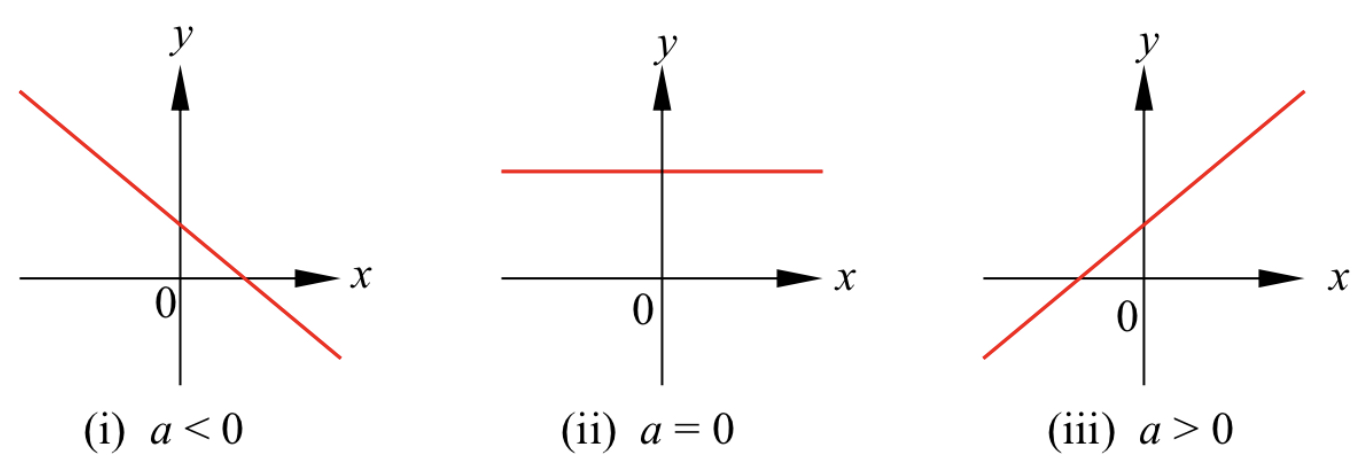
\includegraphics[scale=0.25]{Picture17.png}
\caption{  The graph of the function $f(x)=ax+b$ when (i) $a<0$, (ii) $a=0$ and (iii) $a>0$.\fa}\label{figure17}
\end{figure}

  For the function $y=f(x)=ax+b$,  we find that for any two distinct points $x_1$ and $x_2$,
\[\frac{f(x_2)-f(x_1)}{x_2-x_1}=\frac{a(x_2-x_1)}{x_2-x_1}=a.\]
In other words, the change in the $y$ values,
\[\Delta y=y_2-y_1=f(x_2)-f(x_1)\]
is proportional to the change in the $x$-values
\[\Delta x=x_2-x_1,\] with propotionality constant $a$. This constant $a$ is called the rate of change of the function, and it is the slope of the line $y=ax+b$. Its magnitude $|a|$ characterizes how fast $y$ is changing with respect to $x$, and its sign determine the way $y$ changes. When $a>0$,  $y$ increases as   $x$ increases. When $a<0$, $y$ decreases as $x$ increases. 

For a function that is more complicated, such as a quadratic function $y=f(x)=x^2$, we find that
\[\Delta y=f(x_2)-f(x_1)=x_2^2-x_1^2=(x_2+x_1)(x_2-x_1)=(x_2+x_1)\Delta x.\]
In this case, $\Delta y/\Delta x$ is not a constant. It depends on the points $x_1$ and $x_2$. 

In real-life scenario, functions are used to describe the dependence of a variable on the other. For example, if one wants to record the distance that has been travelled by an object,  the independent variable is the time $t$, while the dependent variable is the distance $s$. In this case, one obtains a function $s=s(t)$. The average speed the object is travelling between the time $t=t_1$ and the time $t=t_2$ is
\[\frac{s(t_2)-s(t_1)}{t_2-t_1}.\]In general, one cannot expect that this speed is a constant. If we are interested in the instantaneous speed that the object is travelling at time $t=t_1$, one can fix $t_1$ and  take  $ t_2$ to be closer and closer to $t_1$, and study the behaviour of the average speed. This leads to the concept of derivatives.


\section{Derivatives }\label{sec3.1}

The derivative of a function $y=f(x)$ is a measure of the rate of change of the $y$-values with respect to the change in the $x$- values. To be able to measure this rate of change at a particular point $x_0$, the function has to be defined in a neighbourhood of the point $x_0$. Henceforth, when we define derivatives, we will assume that the function is defined on an open interval $(a, b)$. This includes the case where $a$ is $-\infty$ or $b$ is $\infty$.

\begin{definition}{Derivatives}
  Given a function $f:(a,b)\to \mathbb{R}$ and a point $x_0$ in the interval $(a, b)$, the derivative of $f$ at $x_0$ is defined to be the limit
\[\lim_{x\rightarrow x_0} \frac{f(x)-f(x_0)}{x-x_0}\] if it exists. If the limit exists, we say that $f$ is differentiable at $x_0$, and its derivative a $x_0$ is denoted by $f'(x_0)$. Namely,
\[f'(x_0)=\lim_{x\rightarrow x_0} \frac{f(x)-f(x_0)}{x-x_0}.\]

\end{definition}


Notice that in defining the derivative of a function $f(x)$ at a point $x_0$, the function that we are taking limit of is the function
\[g(x)=\frac{f(x)-f(x_0)}{x-x_0},\]
which is defined on the set $D=(a,b)\setminus\{x_0\}$. It is easy to check that $x_0$ is indeed a limit point of the set  $D$. The function $g(x)$ is the quotient of the function $p(x)=f(x)-f(x_0)$ and the function $q(x)=x-x_0$. It is not defined at $x=x_0$ since $q(x_0)=0$. Moreover, since  $\di\lim_{x\rightarrow x_0}q(x)=q(x_0)=0$,  a necessary condition for $f$ to be differentiable at the point $x_0$ is $\di\lim_{x\rightarrow x_0}p(x)=0$, which says that  the function $f(x)$ is continuous at $x_0$.

\begin{theorem}[label=23021302]{Differentiability Implies Continuity}
Let $x_0$ be a point in the open interval $(a, b)$. If the function $f:(a,b)\to \mathbb{R}$ is differentiable at $x_0$, it is continuous  at $x_0$.
\end{theorem}
\begin{myproof}{Proof}
If $f$ is differentiable at $x_0$, the limit
\[f'(x_0)=\lim_{x\rightarrow x_0} \frac{f(x)-f(x_0)}{x-x_0}\] exists. By limit laws,
\[\lim_{x\to x_0}(f(x)-f(x_0))=\lim_{x\rightarrow x_0} \frac{f(x)-f(x_0)}{x-x_0}\lim_{x\to x_0}(x-x_0)=f'(x_0)\times 0=0.\]
Hence,
\[\lim_{x\to x_0}f(x)=f(x_0),\] which proves that $f$ is continuous at $x_0$.
\end{myproof}

\begin{highlight}{}
By writing $x=x_0+h$, where $h=x-x_0$ is the change in the $x$-values, we can write the derivative of a function $f:(a,b)\to\mathbb{R}$ at a point $x_0$ as
\[f'(x_0)=\lim_{h\to 0}\frac{f(x_0+h)-f(x_0)}{h}.\]
The continuity of the function $f$ at the point $x_0$ is then equivalent to
\[\lim_{h\to 0}f(x_0+h)=f(x_0).\]
\end{highlight}


\begin{definition}{Differentiable Functions}
We say that a function $f:(a,b)\to \mathbb{R}$ is {\bf differentiable} if it is differentiable at all points in $(a,b)$. In this case, the derivative of $f$ is the function $f':(a,b)\to\mathbb{R}$, where
\[f'(x)=\lim_{h\to 0}\frac{f(x+h)-f(x)}{h}.\]
\end{definition}
Let us look at the simplest example where $f(x)=ax+b$.
\begin{example}
{}
Let $f:\mathbb{R}\to\mathbb{R}$ be the function $f(x)=ax+b$. For any $x$ and $x_0$ where $x\neq x_0$, we have
\[\frac{f(x)-f(x_0)}{x-x_0}=a.\]
This implies that
\[f'(x_0)=\lim_{x\to x_0}\frac{f(x)-f(x_0)}{x-x_0}=a.\] Hence, $f$ is a differentiable function and its derivative is
\[f'(x)=a\hspace{1cm}\text{for all}\;x\in\mathbb{R}.\]
\end{example}

Now let us look at a quadratic function.
\begin{example}[label=23021301]{}
Let $f:\mathbb{R}\rightarrow \mathbb{R}$ be the function $f(x)=x^2$. Show that $f$ is differentiable and find its derivative.
\end{example}
\begin{solution}{Solution}
For any real number $x$,
\begin{align*}
f'(x)&=\lim_{h\to 0}\frac{f(x+h)-f(x)}{h}\\
&=\lim_{h\to 0}\frac{(x+h)^2-x^2}{h}\\
&=\lim_{h\to 0}\frac{2xh+h^2}{h}\\
&=\lim_{h\to 0}\;(2x+h)\\
&=2x.
\end{align*}This shows that $f$ is differentiable and its derivative is $f'(x)=2x$.
\end{solution}

 Finding derivative is finding the limit of 
\[m_{x;x_0}=\frac{f(x)-f(x_0)}{x-x_0}\] as $x$ approaches $x_0$. Since $m_{x;x_0}$ is the slope of the secant line joining the two points $(x_0, f(x_0))$ and $(x,f(x))$ on the graph of the function, in the limit $x\to x_0$, we obtain a straight line that only touches the graph in a neighbourhood of the point $(x_0, f(x_0))$ at this point. This line is called the tangent line of the curve $y=f(x)$ at the point $(x_0, f(x_0))$.

 \begin{figure}[ht]
\centering
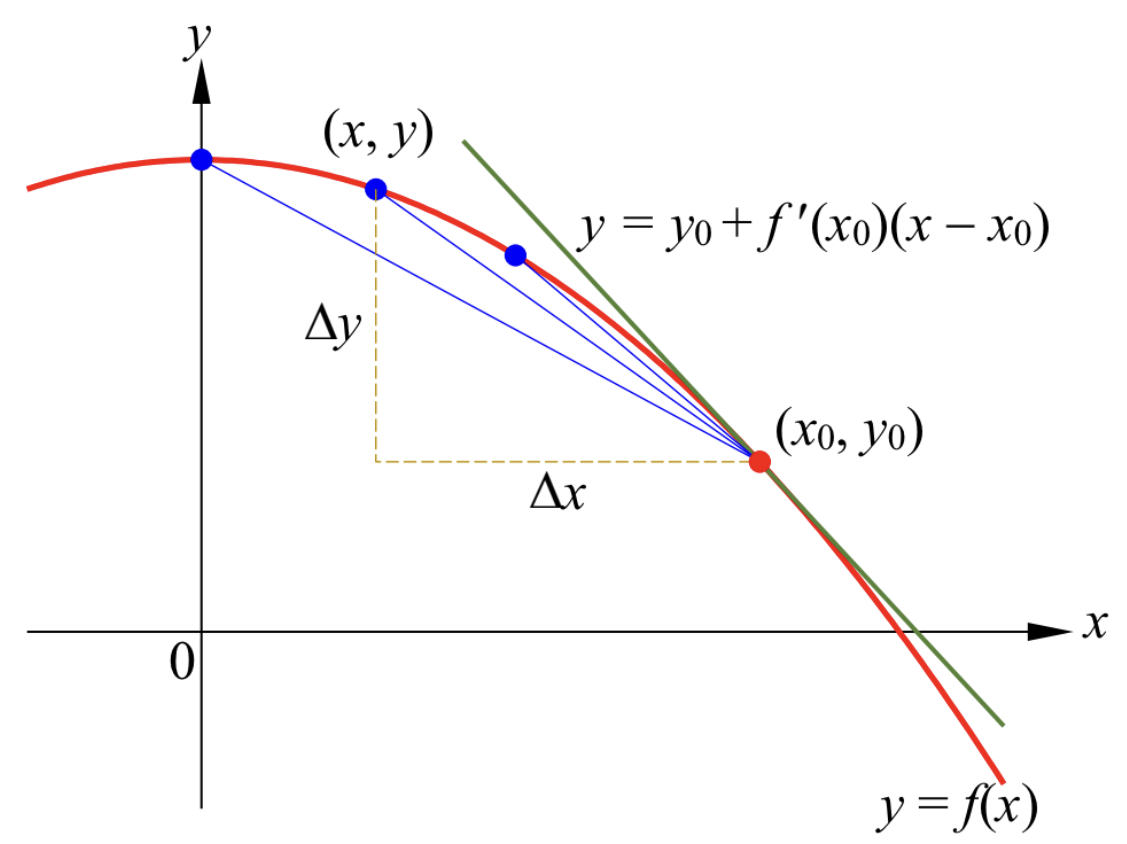
\includegraphics[scale=0.2]{Picture18.png}
\caption{  Derivative as slope of tangent line. \fa}\label{figure18}
\end{figure}

\begin{definition}{Tangent Line}
Let $x_0$ be a point in the interval $(a,b)$. If the function $f:(a,b)\to\mathbb{R}$ is  differentiable at $x_0$, then the tangent line to the curve $y=f(x)$ at the point $(x_0, f(x_0))$ is
\[y=y_0+f'(x_0)(x-x_0).\]
\end{definition}


\begin{example}{}
We have found in Example \ref{23021301} that the derivative of the function $f(x)=x^2$ is $f'(x)=2x$. At the point $x=3$, $f(3)=9$ and $f'(3)=6$. Hence, the equation of the tangent line to the curve $y=x^2$ at the point $(3,9)$ is
\[y=9+6(x-3)=6x-9.\]
\end{example}

Theorem \ref{23021302} says that if a function $f:(a,b)\to \mathbb{R}$ is differentiable at $x_0$, then it is continuous at $x_0$. A natural question to ask is whether the converse is true. The answer is no, as shown by the following classical example.

\begin{example}[label=23021303]{}
Consider the function $f:\mathbb{R}\to\mathbb{R}$, $f(x)=|x|$. We have seen in Chapter \ref{ch2} that this is a continuous function. Let $x_0$ be a point in $\mathbb{R}$.

\textbf{Case 1:} If $x_0>0$, then for any $x$ in the neighbourhood $(0, \infty)$ of $x_0$, $f(x)=|x|=x$.  It follows that
\[\lim_{x\to x_0}\frac{f(x)-f(x_0)}{x-x_0}=\lim_{x\to x_0}\frac{x-x_0}{x-x_0}=1.\]
This implies that $f$ is differentiable at $x_0$ and $f'(x_0)=1$.

\textbf{Case 2:} If $x_0<0$, then for any $x$ in the neighbourhood $(-\infty, 0)$ of $x_0$, $f(x)=|x|=-x$.  It follows that 
\[\lim_{x\to x_0}\frac{f(x)-f(x_0)}{x-x_0}=\lim_{x\to x_0}\frac{-x-(-x_0)}{x-x_0}=-\frac{x-x_0}{x-x_0}=-1.\]
This implies that $f$ is differentiable at $x_0$ and $f'(x_0)=-1$.

\textbf{Case 3:} When $x_0=0$, we find that
\[\lim_{x\to 0^+}\frac{f(x)-f(0)}{x-0}=\lim_{x\to 0^+}\frac{x}{x}=1,\]
\[\lim_{x\to 0^-}\frac{f(x)-f(0)}{x-0}=\lim_{x\to 0^-}\frac{-x}{x}=-1.\]
This implies that the limit 
\[\lim_{x\to 0}\frac{f(x)-f(0)}{x-0}\] does not exist. Hence, $f$ is not differentiable at $x=0$.
\end{example}

Graphically, we find that the curve $y=|x|$ has a "sharp turn" at the point $(0,0)$, and there is no well-defined tangent there (see Figure \ref{figure19}).

 \begin{figure}[ht]
\centering
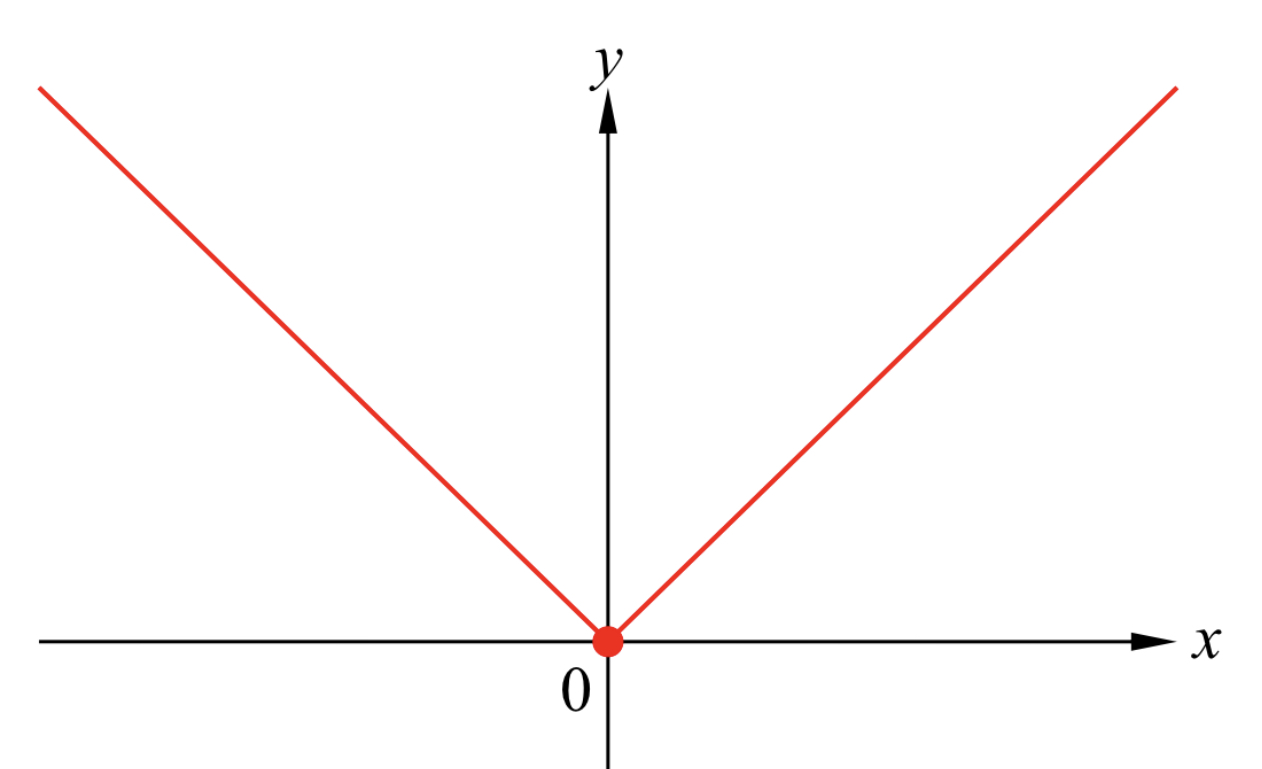
\includegraphics[scale=0.18]{Picture19.png}
\caption{  The graph of the function $f(x)=|x|$ has a "sharp turn" at $x=0$. \fa}\label{figure19}
\end{figure}

\begin{remark}{Left Derivatives and Right Derivatives}

We can use left limits and right limits to define left derivatives and right derivatives.  
Let $f:[a,b]\rightarrow \mathbb{R}$ be a function defined on the closed interval $[a,b]$.

\begin{enumerate}[1.]
\item 
For any $x_0\in (a, b]$, we say that the function is left-differentiable at $x_0$ provided that the left derivative at $x_0$, $f_-'(x_0)$, defined as the left limit
\[f_-'(x_0)=\lim_{x\to x_0^-}\frac{f(x)-f(x_0)}{x-x_0},\] exists.  

\item 
For any $x_0\in [a, b)$, we say that the function is right-differentiable at $x_0$ provided that the right derivative at $x_0$, $f_+'(x_0)$, defined as the right limit
\[f_+'(x_0)=\lim_{x\to x_0^+}\frac{f(x)-f(x_0)}{x-x_0},\] exists.  

\item For any $x_0\in (a, b)$, $f$ is differentiable at $x_0$ if and only if it is both left differentiable and right differentiable at $x_0$.

\item We say that the function  $f:[a,b]\rightarrow \mathbb{R}$ is differentiable if it is differentiable at all $x_0\in (a, b)$, right differentiable at $a$ and left differentiable at $b$.
\end{enumerate}

\end{remark}
 In the following, we will mainly discuss derivatives of functions defined on open intervals. The extension to closed intervals is straighforward by considering the one-sided derivatives at the end points.


\begin{example}{\linkt Example \ref{23021303} Revisited}
The function $f(x)=|x|$ is left differentiable and right differentiable at $x=0$, with 
\[f_-'(0)=-1,\hspace{1cm}f_+'(0)=1.\]
It is not differentiable at $x=0$ since $f_-'(0)\neq f_+'(0)$.
\end{example}

\begin{highlight}{Leibniz Notation for Derivatives}
For the function $y=f(x)$, its derivative $f'(x)$ is also denoted by $\di \frac{dy}{dx}$ or $\di \frac{d}{dx}f(x)$.
\end{highlight}

For example, in Example \ref{23021301}, we have shown that
\[\frac{d}{dx} x^2=2x.\]

In the following, we are going to derive derivative formulas. 
The simplest   derivative formula is the one for the function $f(x)=x^n$, where $n$ is a positive integer.
\begin{proposition}{}
Let $n$ be a positive integer. The function $f(x)=x^n$ is differentiable with derivative 
\[\frac{d}{dx}x^n=nx^{n-1}.\]
\end{proposition}
\begin{myproof}{Proof}
We use the formula
\[x^n-x_0^n=(x-x_0)(x^{n-1}+x^{n-2}x_0+\cdots+xx_0^{n-2}+x_0^{n-1}).\]
Let $f(x)=x^n$. Then\bp
\begin{align*}
 f'(x_0)&=\lim_{x\to x_0}\frac{f(x)-f(x_0)}{x-x_0}\\
&=\lim_{x\to x_0}\frac{x^n-x_0^n}{x-x_0}\\
&=\lim_{x\to x_0}\left(x^{n-1}+x^{n-2}x_0+\cdots+xx_0^{n-2}+x_0^{n-1}\right)\\
&=\underbrace{x_0^{n-1}+x_0^{n-1}+\cdots+x_0^{n-1}+x_0^{n-1}}_{n \;\text{terms}}\\
&=nx_0^{n-1}.
\end{align*}
\end{myproof}

Now let us look at the square root function.
\begin{example}{}
Determine the points where the function $f:[0, \infty)\to\mathbb{R}$, $f(x)=\sqrt{x}$ is differentiable, and find the derivatives at those points.
\end{example}
\begin{solution}{Solution}
First we consider the case where $x_0>0$. When $x>0$ and $x\neq x_0$,
\begin{equation}\label{eq230213_4}
\frac{f(x)-f(x_0)}{x-x_0}=\frac{\sqrt{x}-\sqrt{x_0}}{x-x_0}=\frac{1}{\sqrt{x}+\sqrt{x_0}}.
\end{equation}
Hence, 
\[f'(x_0)=\lim_{x\to x_0}\frac{f(x)-f(x_0)}{x-x_0}=\lim_{x\to x_0}\frac{1}{\sqrt{x}+\sqrt{x_0}}=\frac{1}{2\sqrt{x_0}}.\]
This shows that $f$ is differentiable at $x_0$ with derivative $f'(x_0)=\di \frac{1}{2\sqrt{x_0}}$.

For $x_0=0$, we can only consider the right derivative. When $x>0$,
the formula \eqref{eq230213_4} still holds. However, the limit
\[\lim_{x\rightarrow 0^+}\frac{f(x)-f(0)}{x-0}=\lim_{x\to 0^+}\frac{1}{\sqrt{x}}\] does not exist. Hence, the function $f(x)=\sqrt{x}$ is not differentiable at $x=0$.

\end{solution}

 \begin{figure}[ht]
\centering
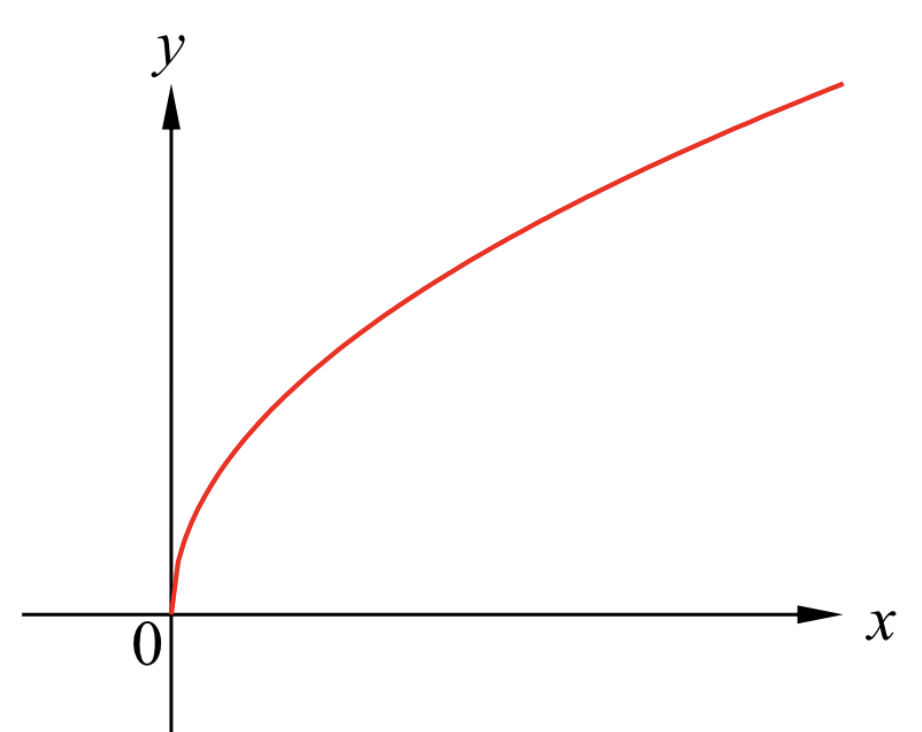
\includegraphics[scale=0.18]{Picture20.png}
\caption{  The function $f(x)=\sqrt{x}$ is not differentiable at $x=0$. \fa}\label{figure20}
\end{figure}

Using limit laws, one can find derivatives of linear combinations, products and quotients of  functions.
\begin{proposition}[label=23021305]{Linearity of Derivatives}
Let $x_0$ be a point in $(a, b)$. Given that the functions $f:(a,b)\to \mathbb{R}$ and $g:(a,b)\to \mathbb{R}$ are differentiable at $x_0$. For any constants $\alpha$ and $\beta$, the function $\alpha f+\beta g:(a,b)\rightarrow\mathbb{R}$ is also differentiable at $x_0$ and
\[(\alpha f+\beta g)'(x_0)=\alpha f'(x_0)+\beta g'(x_0).\]

\end{proposition}

\begin{myproof}{Proof}
This is straightforward derivation from the limit laws. By assumption, we have
\[f'(x_0)=\lim_{x\to x_0}\frac{f(x)-f(x_0)}{x-x_0}\quad\text{and}\quad g'(x_0)=\lim_{x\to x_0}\frac{g(x)-g(x_0)}{x-x_0}.\]
It follows that
\begin{align*}
(\alpha f+\beta g)'(x_0)&=\lim_{x\to x_0}\frac{(\alpha f+\beta g)(x)-(\alpha f+\beta g)(x_0)}{x-x_0}\\
&=\lim_{x\to x_0}\left(\alpha\frac{f(x)-f(x_0)}{x-x_0}+\beta\frac{g(x)-g(x_0)}{x-x_0}\right)\\
&=\alpha \lim_{x\to x_0}\frac{f(x)-f(x_0)}{x-x_0}+\beta \lim_{x\to x_0}\frac{g(x)-g(x_0)}{x-x_0}\\
&=\alpha f'(x_0)+\beta g'(x_0).
\end{align*}
\end{myproof}

This formula can be extended to $k$ functions for any positive integer $k$. If $f_1,  \ldots, f_k$ are functions defined on $(a,b)$ and differentiable at the point $x_0$, then for any constants $c_1, \ldots, c_k$, the function $c_1 f_1+\ldots+c_k f_k$ is also differentiable at $x_0$, and
\[(c_1 f_1+\ldots+c_k f_k)'(x_0)=c_1f_1'(x_0)+\ldots+c_kf_k'(x_0).\]

\begin{proposition}[label=23021306]{Product  Rule for Derivatives}
Let $x_0$ be a point in $(a, b)$. Given that the functions $f:(a,b)\to \mathbb{R}$ and $g:(a,b)\to \mathbb{R}$ are differentiable at $x_0$,   the function $(fg) :(a,b)\rightarrow\mathbb{R}$ is also differentiable at $x_0$ and
\[(fg)'(x_0)=  f'(x_0)g(x_0)+f(x_0) g'(x_0).\]

\end{proposition}

\begin{myproof}{Proof}
Again, we are given that
\[f'(x_0)=\lim_{x\to x_0}\frac{f(x)-f(x_0)}{x-x_0}\quad\text{and}\quad g'(x_0)=\lim_{x\to x_0}\frac{g(x)-g(x_0)}{x-x_0}.\] Since differentiability implies continuity, we have
\[\lim_{x\to x_0}f(x)=f(x_0) \quad\text{and}\quad \lim_{x\to x_0}g(x)=g(x_0).\]
Just like the proof of the product rule for limits, we need to do some manipulations.
\[f(x)g(x)-f(x_0)g(x_0)=(f(x)-f(x_0))g(x_0)+f(x)(g(x)-g(x_0)).\]
It follows that
\begin{align*}
(fg)'(x_0)&=\lim_{x\to x_0}\frac{f(x)g(x)-f(x_0)g(x_0)}{x-x_0}\\
&=\lim_{x\to x_0}\left(\frac{f(x)-f(x_0)}{x-x_0}g(x_0)+f(x)\frac{g(x)-g(x_0)}{x-x_0}\right)\\
&=\lim_{x\to x_0} \frac{f(x)-f(x_0)}{x-x_0}\lim_{x\to x_0} g(x_0)+\lim_{x\to x_0} f(x)\lim_{x\to x_0}\frac{g(x)-g(x_0)}{x-x_0}\\
&=f'(x_0)g(x_0)+f(x_0)g'(x_0).
\end{align*}
\end{myproof}
For a different perspective, we denote $f(x_0)$ and $g(x_0)$ by $u$ and $v$ respectively, and let
\[\Delta u =f(x)-f(x_0),\hspace{1cm} \Delta v=g(x)-g(x_0).\]
Then
\begin{align*}
f(x)g(x)-f(x_0)g(x_0)&=(u+\Delta u)(v+\Delta v)-uv\\
&=v\Delta u+u\Delta v +\Delta u\Delta v.
\end{align*}After didiving by $\Delta x=x-x_0$, the term $\Delta u\Delta v/\Delta x$ vanishes in the limit $\Delta x\to 0$, and we obtain the product rule.

\begin{highlight}{General Product Rule}
The product rule for derivatives can be expressed as
\[\frac{d}{dx}(uv)=v\frac{du}{dx}+u\frac{dv}{dx}.\] 
In general, when we have $k$ functions $u_1, u_2, \ldots, u_k$,
the product rule says that
\[\frac{d}{dx}(u_1u_2\cdots u_k)=(u_2\cdots u_k)\frac{d u_1}{dx}
+(u_1u_3\cdots u_k)\frac{du_2}{dx}+\cdots+(u_1\cdots u_{k-1})\frac{du_k}{dx}.\]
This can be proved by induction on $k$.
\end{highlight}
Notice that the formula
\[\frac{d}{dx}x^n=nx^{n-1}, \quad\text{where}\;n\in\mathbb{Z}^+ \] follows from the general product rule and $\di\frac{d}{dx}x=1$.

Finally we turn to the quotient rule.
\begin{proposition}[label=23021307]{Quotient Rule for Derivatives} 
Let $x_0$ be a point in $(a, b)$. Given that the functions $f:(a,b)\to \mathbb{R}$ and $g:(a,b)\to \mathbb{R}$ are differentiable at $x_0$, and $g(x)\neq 0$ for all $x$ in $(a,b) $. Then the function $(f/g):(a,b)\to\mathbb{R}$ is differentiable at $x_0$ and
\[\left(\frac{f}{g}\right)'(x_0)=\frac{f'(x_0)g(x_0)-f(x_0)g'(x_0)}{g (x_0)^2}.\]
\end{proposition}The assumption $g(x)\neq 0$ for all $x$ in $ (a,b)$ is to make sure that the function $f/g$ is well-defined on $(a,b)$. In practice, we only need $g(x_0)\neq 0$ and $g$ is differentiable at $x_0$. For  then we find that $g$ is continuous at $x_0$. The assumption $g(x_0)\neq 0$ will imply that $g(x)\neq 0$ in a neighbourhood of $x_0$.
\begin{myproof}{Proof}First, notice that
\begin{align*}
\frac{f(x)}{g(x)}-\frac{f(x_0)}{g(x_0)}&=\frac{f(x)g(x_0)-f(x_0)g(x)}{g(x)g(x_0)}\\&=\frac{(f(x)-f(x_0))g(x_0)-f(x_0)(g(x)-g(x_0))}{g(x)g(x_0)}.
\end{align*}Using the same reasoning as in the proof of the product rule, we obtain
\begin{align*}
 \left(\frac{f}{g}\right)'(x_0) &=\lim_{x\to x_0}\frac{1}{g(x)g(x_0)}\\&\quad \times\left\{g(x_0)\lim_{x\to x_0}\frac{f(x)-f(x_0)}{x-x_0}-f(x_0)\lim_{x\to x_0}\frac{g(x)-g(x_0)}{x-x_0}\right\}\\
&=\frac{f'(x_0)g(x_0)-f(x_0)g'(x_0)}{g (x_0)^2}.
\end{align*}
\end{myproof}
Again, using the $u$ and $v$ notations, we have
\[\frac{u+\Delta u}{v+\Delta v}-\frac{u}{v}=\frac{(u+\Delta u)v-(v+\Delta v)u}{v(v+\Delta v)}=\frac{v\Delta u-u\Delta v}{v(v+\Delta v)}.\] This gives a different perspective on the quotient rule.

Let us use the quotient rule to derive the derivative for $f(x)=x^n$, when $n$ is a negative integer. 

\begin{proposition}[label=prop230215_1]{}
For any integer $n$,
\begin{equation}\label{eq230213_8}\frac{d}{dx}x^n =nx^{n-1}.\end{equation}

\end{proposition}
\begin{myproof}{Proof}
We have proved the formula   \eqref{eq230213_8} when $n\geq 0$. When $n<0$, let $m=-n$. Then $m$ is a positive integer.  
By quotient rule, we have
\[\frac{d}{dx}x^n=\frac{d}{dx}\frac{1}{x^m}=\frac{x^m \di \frac{d}{dx} 1- \frac{d}{dx}x^m}{x^{2m}}=-\frac{mx^{m-1}}{x^{2m}}=-\frac{m}{x^{m+1}}=nx^{n-1}.\]
Hence, the formula \eqref{eq230213_8} also holds when $n$ is a negative integer.  
\end{myproof}

\begin{definition}{Higher Order Derivatives}
If the function $f:(a,b)\to\mathbb{R}$ is differentiable, its derivative $f':(a,b)\to\mathbb{R}$ is also a function  defined on $(a, b)$. We can investigate whether $f'$ is differentiable. If $f'$ is differentiable at a point $x_0$ in $(a, b)$, we denote its derivative by $f''(x_0)$, called the second (order) derivative of the function $f$ at $x_0$. 

In the same way, we can define the $n^{\text{th}}$-order derivative of the function $y=f(x)$ at  a point $x_0$ for any positive integer $n$. We use the notation \[f^{(n)}(x)\quad\text{or}\quad\frac{d^n y}{dx^n}\] to denote the $n^{\text{th}}$-derivative of the function $y=f(x)$. It is defined recursively by
\[f^{(n)}(x)=\lim_{h\to 0}\frac{f^{(n-1)}(x+h)-f^{(n-1)}(x)}{h},\]
where by default, $f^{(0)}(x)=f(x)$.

We say that a function $f:(a,b)\rightarrow\mathbb{R}$ is $n$ times differentiable if $f^{(n)}(x)$ exists for all $x$ in $(a,b)$. A function is infinitely differentiable if it is $n$ times differentiable for any positive integer $n$.
\end{definition}

\begin{example}{}
Polynomial functions are infinitely differentiable. Moreover, if the degree of a polynomial $p(x)$ is  $n$, then
$p^{(k)}(x)=0$ for all $k\geq n+1$.
\end{example}

\begin{example}[label=23021401]{}
Define the function $f:\mathbb{R}\to\mathbb{R}$ by
\[f(x)=\begin{cases} ax^2,\quad &\text{if}\;x< 1,\\
x+\di \frac{b}{x},\quad &\text{if}\; x\geq 1.\end{cases}
\]Find the values of $a$ and $b$ so that $f$ is differentiable.

\end{example}
\begin{solution}{Solution}
The function $f$ is differentiable at any point  $x_0$ in the interval $(-\infty, 1)$ or the interval $(1, \infty)$.

For $f$  to be  differentiable, $f$ has to be continuous and differentiable at $x=1$. For $f$ to be continuous at $x=1$, we must have
\[\lim_{x\rightarrow 1^-}f(x)=\lim_{x\rightarrow 1^+}f(x).\]
This gives
\[a=1+b.\]
For $f$ to be differentiable at $x=1$, we must have
\[\lim_{x\rightarrow 1^-}\frac{f(x)-f(1)}{x-1}=\lim_{x\rightarrow 1^+}\frac{f(x)-f(1)}{x-1}.\]
Notice that
\[\lim_{x\rightarrow 1^-}\frac{f(x)-f(1)}{x-1}=\left.\frac{d}{dx}\right|_{x=1}ax^2=2a,\]
\[\lim_{x\rightarrow 1^+}\frac{f(x)-f(1)}{x-1}=\left.\frac{d}{dx}\right|_{x=1}\left(x+\frac{b}{x}\right)=1-b.\]
Hence, we must have
\[2a=1-b.\]
Solving for $a$ and $b$, we have 
\[a= \frac{2}{3},\;b=-\frac{1}{3}.\]
\end{solution}

\vp
 \begin{figure}[ht]
\centering
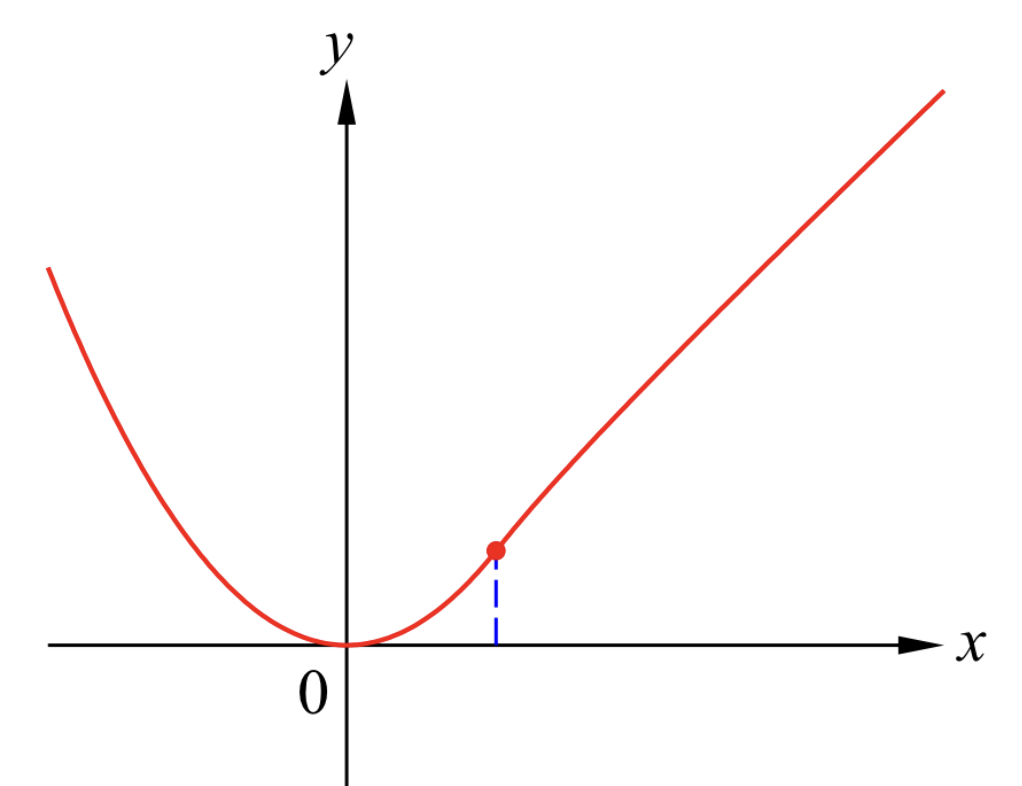
\includegraphics[scale=0.2]{Picture21.png}
\caption{  The function $f(x)$ defined in Example \ref{23021401}. \fa}\label{figure21}
\end{figure}

\vp
 
\noindent
{\bf \large Exercises  \thesection}
\setcounter{myquestion}{1}
\begin{question}{\themyquestion} 
Define the function $f:\mathbb{R}\to\mathbb{R}$ by
\[f(x)=\begin{cases} ax^2+ x,\quad &\text{if}\;x< 1,\\
bx+\di \frac{3 }{x^2},\quad &\text{if}\;x\geq 1.\end{cases}
\]Find the values of $a$ and $b$ so that $f$ is differentiable.
\end{question}
\atc
\begin{question}{\themyquestion} 
Let $x_0$ be a point in $(a, b)$. Given that $f:[a,b]\to\mathbb{R}$ is a continuous function defined on $[a, b]$ and differentiable at $x_0$. Let
$g:[a,b]\to\mathbb{R}$ be the function defined by
\[g(x)=\begin{cases} \di\frac{f(x)-f(x_0)}{x-x_0},\quad& \text{if}\;x\in [a,b]\setminus\{ x_0\}\\f'(x_0),\quad & \text{if}\;x=x_0.\end{cases}\]Show that $g:[a,b]\to\mathbb{R}$ is a continuous function.
\end{question}
 
\atc
\begin{question}{\themyquestion} 
Let $x_0$ be a point in $(a, b)$ and let   $f:(a,b)\to\mathbb{R}$ be a function defined on $(a, b)$. 
\begin{enumerate}[(a)]
\item If $f:(a,b)\to\mathbb{R}$ is differentiable at $x_0$, show that
\[\lim_{h\to 0}\frac{f(x_0+h)-f(x_0-h)}{2h}=f'(x_0).\]
\item If the limit \[\lim_{h\to 0}\frac{f(x_0+h)-f(x_0-h)}{2h}\] exists, is $f$ necessarily differentiable at $x_0$?
\end{enumerate}
\end{question}


\vp

\section{Chain Rule and Derivatives of Inverse Functions}\label{sec3.2}

In this section, we are going to derive derivative formulas for composite functions and inverse functions. First we discuss a different perspective for differentiability of a function at a point.

\begin{highlight}{Differentiability}
Let $x_0$ be a point in the interval $(a, b)$ and let $f:(a,b)\rightarrow \mathbb{R}$ be a function defined on $(a, b)$. 
If $f$ is differentiable at $x_0$, then
\[f'(x_0)=\lim_{h\to 0}\frac{f(x_0+h)-f(x_0)}{h}.\]
This implies that
\[\lim_{h\to 0}\frac{f(x_0+h)-f(x_0)-f'(x_0)h}{h}=0.\]
Conversely, if there is a number $c$ such that
\[\lim_{h\to 0}\frac{f(x_0+h)-f(x_0)-ch}{h}=0,\]
limit laws imply that
\[c=\lim_{h\to 0}\frac{f(x_0+h)-f(x_0)}{h}.\]
This implies that $f$ is differentiable at $x_0$ and $f'(x_0)=c$.
In other words, the function $f$ is differentiable at $x_0$ if and only if there is a number $c$ such that
\[\lim_{h\to 0}\frac{f(x_0+h)-f(x_0)-ch}{h}=0.\]

Since $x_0\in (a, b)$, there is an $r>0$ such that $(x_0-r, x_0+r)\subset (a,b)$.  For a given real number $c$, let
$\varepsilon:(-r,r)\to\mathbb{R}$ be the function defined by
\[\varepsilon(h)=\frac{f(x_0+h)-f(x_0)-ch}{h}.\] \end{highlight}\begin{highlight}{} Then the differentiability of $f$ at $x_0$ is equivalent to $\di\lim_{h\rightarrow 0}\varepsilon(h)=0$.
Hence, $f:(a,b)\to\mathbb{R}$ is differentiable at $x_0$ if and only if there is a number $c$ and a function $\varepsilon(h)$ such that
\[f(x_0+h)=f(x_0)+ch+h\varepsilon(h),\]
and
\[\varepsilon(h)\to 0\quad\text{when}\;h\to 0.\]
\end{highlight}

\begin{theorem}{Chain Rule}
Given that  $f:(a,b)\to \mathbb{R}$ and $g:(c,d)\to\mathbb{R}$ are  functions such that $f(a,b)\subset (c,d)$. If $x_0$ is a point in $(a,b)$, $f$ is differentiable at $x_0$, $g$ is differentiable at $f(x_0)$, then the composite function $ (g\circ f):(a, b)\to \mathbb{R}$ is differentiable at $x_0$ and 
\[(g\circ f)'(x_0)=g'(f(x_0))f'(x_0).\]

\end{theorem}
\begin{myproof}{Proof}
Let  $y_0=f(x_0)$, and define the functions $\varepsilon_1(h)$ and $\varepsilon_2(k)$ by
\begin{align*}
\varepsilon_1(h)&=\frac{f(x_0+h)-f(x_0)-f'(x_0)h}{h},\\
\varepsilon_2(k)&=\frac{g(y_0+k)-g(y_0)-g'(y_0)k}{k}.
\end{align*}Since $f$ is differentiable at $x_0$ and $g$ is differentiable at $y_0$, we have
$\di\lim_{h\to 0}\varepsilon_1(h)=0$ and $\di \lim_{k\to 0}\varepsilon_2(k)=0$.
Let
\[k(h)=f(x_0+h)-f(x_0)=f'(x_0)h+\varepsilon_1(h)h.\] Then by the definitions of $\varepsilon_1(h)$ and $\varepsilon_2(k)$,
\begin{align*}
(g\circ f)(x_0+h)-(g\circ f)(x_0)&=g(y_0+k(h))-g(y_0)\\
&=g'(y_0)k(h)+\varepsilon_2(k(h))k(h)\\
&=g'(y_0)f'(x_0)h+\varepsilon_3(h)h,
\end{align*}\bp
where 
\[\varepsilon_3(h)=g'(y_0)\varepsilon_1(h)+\varepsilon_2(k(h))\frac{k(h)}{h}.\]
Since $f$ is differentiable at $x_0$, \[\lim_{h\to 0}\frac{k(h)}{h}=\lim_{h\to 0}\frac{f(x_0+h)-f(x_0)}{h}=f'(x_0).\] This implies that $\di\lim_{h\rightarrow 0}k(h) =0$. By limit law  for composite functions,
\[\lim_{h\to 0}\varepsilon_2(k(h))=\lim_{k\to 0}\varepsilon_2(k)=0.\]
Limit laws then imply that
\[\lim_{h\to 0}\frac{(g\circ f)(x_0+h)-(g\circ f)(x_0)-g'(y_0)f'(x_0)h}{h}=\lim_{h\to 0}\varepsilon_3(h)=0.\]
This proves that the function $g\circ f$ is differentiable at $x_0$ and 
\[(g\circ f)'(x_0)=g'(y_0)f'(x_0)=g'(f(x_0))f'(x_0).\]
\end{myproof}
Heuristically, if we let $u=f(x)$ and $y=g(u)=g(f(x))$,   chain rule says that
\[\frac{dy}{dx}=\frac{dy}{du}\times\frac{du}{dx},\]
which is the limit of 
\[\frac{\Delta y}{\Delta x}=\frac{\Delta y}{\Delta u}\times\frac{\Delta u}{\Delta x}\]when $\Delta x\to 0$.
The rigorous proof we give above do not use this because we might face the problem that $\Delta u=f(x)-f(x_0)$ can be zero even when $x\neq x_0$. 

\begin{example}
{}
Let $f:\mathbb{R}\to\mathbb{R}$ be a differentiable function and let $a$ be a constant. Show that the function $g:\mathbb{R}\to\mathbb{R}$ defined by $g(x)=f(ax)$ is differentiable, and $g'(x)=af'(ax)$.



\end{example}
\begin{solution}{Solution}
The function $u:\mathbb{R}\to\mathbb{R}$, $u(x)=ax$ is differentiable with $u'(x)=a$. By  chain rule, the function $g(x)=(f\circ u)(x)$ is also differentiable and
\[g'(x)=f'(u(x))u'(x)=af'(ax).\]
\end{solution}

\begin{example}{}
Given that the function $f:(0,2)\to \mathbb{R}$ is differentiable at $x=1$ and $f'(1)=a$, find the value of
\[\lim_{x\rightarrow 1}\frac{f(x^3)-f(1)}{x-1}\] in terms of $a$.
\end{example}
\begin{solution}{Solution}
Let $g(x)=x^3$. Then $g(1)=1$ and $g$ is differentiable at $x=1$ with $g'(1)=3$.
\[\lim_{x\rightarrow 1}\frac{f(x^3)-f(1)}{x-1}=\lim_{x\rightarrow 1}\frac{(f\circ g)(x )-(f\circ g)(1)}{x-1}.\]
Since $g$ is differentiable at $x=1$ and  $f$ is differentiable at $g(1)$,   chain rule implies that
\[\lim_{x\rightarrow 1}\frac{f(x^3)-f(1)}{x-1}=(f\circ g)'(1)=f'(g(1))g'(1)=3f'(1)=3a.\]
\end{solution}

Recall that we have proved in Section \ref{sec2.6} that if $I$ is an interval, $f:I\to\mathbb{R}$ is strictly monotonic and continuous, then $f$ is invertible and $f^{-1}:f(I)\to \mathbb{R}$ is also continuous. The strictly monotonicity is a necessary and sufficient condition for a continuous function to be one-to-one. If $x_0$ is a point in the interior of $I$, and $f$ is differentiable at $x_0$, we can ask whether the inverse function $f^{-1}$ is differentiable at the point $y_0=f(x_0)$. 
Since $(f^{-1}\circ f)(x)=x$ for all $x\in I$, if $f^{-1}$ is differentiable at $y_0$,  chain rule implies that
\[(f^{-1})'(y_0)f'(x_0)=(f^{-1})'(f(x_0))f(x_0)=1.\]
Therefore, a necessary condition for $f^{-1}$ to be differentiable at $y_0$ is $f'(x_0)$ cannot be zero. In the following theorem, we show that this condition is also sufficient. 

\begin{theorem}[label=thm230218_9]{Derivative for Inverse Function}
Let $I$ be an open interval containing   $x_0$, and let $f:I\rightarrow\mathbb{R}$ be a function that is strictly monotonic  and continuous. If $f$ is differentiable at $x_0$ and $f'(x_0)\neq 0$, the inverse function $f^{-1}:f(I)\to \mathbb{R}$ is differentiable at $y_0=f(x_0)$, and 
\[(f^{-1})'(y_0)=\frac{1}{f'(x_0)}.\]
\end{theorem}
The formula for $(f^{-1})'(y_0)$ would follow from the chain rule if we know apriori that $f^{-1}$ is   differentiable at $y_0$. The gist of this theorem is to state that $f^{-1}$ is indeed differentiable at $y_0$.

\begin{myproof}{Proof}Without loss of generality, assume that $f$ is strictly increasing. 
By Theorem \ref{23021106}, $f^{-1}:f(I)\to\mathbb{R}$ is also continuous.
There is a  $\delta>0$ so that $[x_0-\delta, x_0+\delta]\subset I$. Then $(f(x_0-\delta), f(x_0+\delta))$ is an open interval in $f(I)$ containing the point $y_0$.  This implies that there is an $r>0$ so that $(y_0-r, y_0+r)\subset f(I)$. For any $k\in (-r, r)$, let 
\[h(k)=f^{-1}(y_0+k)-f^{-1}(y_0).\]Then $h$ is a strictly increasing continuous function of $k$ and  $\di\lim_{k\to 0}h(k)=0$. Notice that
\[y_0+k=f(x_0+h(k)).\]
Therefore,
\[\frac{f^{-1}(y_0+k)-f^{-1}(y_0)}{k}=\frac{h(k)}{f(x_0+h(k))-f(x_0)}.\]
\bp
Hence, by limit laws for quotients and composite functions,
we find that
\begin{align*}
\lim_{k\to 0}\frac{f^{-1}(y_0+k)-f^{-1}(y_0)}{k}&=\frac{1}{\di \lim_{k\rightarrow 0}\frac{f(x_0+h(k))-f(x_0)}{h(k)}}\\&=\frac{1}{\di \lim_{h\rightarrow 0}\frac{f(x_0+h)-f(x_0)}{h}}\\&=\frac{1}{f'(x_0)}.\end{align*}
This proves that $f^{-1}$ is differentiable at $y_0$ and
\[(f^{-1})'(y_0)=\frac{1}{f'(x_0)}.\]

 \end{myproof}

As a corollary, we have the following.
\begin{corollary}{}
Let $I$ be an open interval, and let $f:I\to\mathbb{R}$ be a strictly monotonic differentiable function. If $f'(x)\neq 0 $ for all $x\in I$, then the inverse function $f^{-1}:f(I)\to\mathbb{R}$ is also a strictly monotonic differentiable function with
\[(f^{-1})'(x)=\frac{1}{f'(f^{-1}(x))}.\]
\end{corollary}
 
\begin{example}{}
Let $r$ be a rational number, and let $f:(0,\infty)\to \mathbb{R}$ be the function $f(x)=x^r$. Show that $f$ is differentiable and 
\[f'(x)=rx^{r-1}.\]

\end{example}
\begin{solution}{Solution}
First we consider the case  $r=1/n$, where $n$ is a positive integer. The function $f(x)=x^{1/n}$ is the inverse of the function $g(x)=x^n$, which is differentiable and strictly increasing. Hence, $f(x)=x^{1/n}$ is differentiable and strictly increasing. Moreover, since $g'(x)=nx^{n-1}$, we have
\[f'(x)=\frac{1}{g'(f(x))}=\frac{1}{g'(x^{1/n})}=\frac{1}{n(x^{1/n})^{n-1}}=\frac{1}{n}x^{\frac{1}{n}-1}.\]
Now for a general rational number $r$, there is an integer $p$ and a positive integer $q$ such that
$r=p/q$. It follows that
\[f(x)=(x^p)^{1/q}=(g\circ h)(x),\]
where
\[h(x)=x^p,\hspace{1cm} g(x)=x^{1/q}.\]
By Proposition \ref{prop230215_1}, $h'(x)=px^{p-1}$. We have just shown that $\di g'(x)=\frac{1}{q}x^{\frac{1}{q}-1}$. By chain rule,
\[f'(x)=g'(h(x))h'(x)=\frac{1}{q}\left(x^p\right)^{\frac{1}{q}-1} \times px^{p-1}=\frac{p}{q}x^{\frac{p}{q}-1}=rx^{r-1}.\]
\end{solution}

\vp
\noindent 
{\bf \large Exercises  \thesection}
\setcounter{myquestion}{1}
\begin{question}{\themyquestion}
Given that the function $f:(0,\infty)\to \mathbb{R}$ is defined by
\[f(x)=\frac{1}{\sqrt{4+x^2}}.\]
\begin{enumerate}[(a)]
\item Show that $f$ is one-to-one.
\item Show that $f$ is differentiable.
\item Show that $f^{-1}$ exists and is differentiable.
\item Find $f^{-1}(x)$ and $(f^{-1})'(x)$.
\end{enumerate}
\end{question}

\atc


\begin{question}{\themyquestion}
Let $a$ be a positive number. 
Recall that a function $f:(-a, a)\to\mathbb{R}$ is even if and only if
\[f(-x)=f(x)\hspace{1cm}\text{for all}\;x\in (-a,a);\]
and a function $f:(-a, a)\to\mathbb{R}$ is odd if and only if
\[f(-x)=-f(x)\hspace{1cm}\text{for all}\;x\in (-a,a).\]
Let $f:(-a,a)\to\mathbb{R}$ be a differentiable function.
\begin{enumerate}[(a)]
\item If $f$ is even, show that $f'$ is odd.
\item If $f$ is odd, show that $f'$ is even.

\end{enumerate}
\end{question}
\vp

\section{The Mean Value Theorem  and Local Extrema}\label{sec3.3}

The mean value theorem is one of the most important theorems in analysis. 
We will first prove a special case of the mean value theorem called Rolle's theorem. To prove this, we need the extreme value theorem, which asserts the existence of global maximum and global minimum for a continuous function defined on a closed and bounded interval. As a matter of fact, what we actually need is a local extremum, which we define as follows.

 

\begin{definition}{Local Maximum and Local Minimum}
Let $D$ be a subset of real numbers that contains the point $x_0$, and let $f:D\to\mathbb{R}$ be a function defined on $D$. 
\begin{enumerate}[1.]
\item The point  $x_0$ is a local maximizer of $f$
provided that there is a $\delta>0$ such that for all $x$ in $D$ with $|x-x_0|<\delta$,   we have
\[f(x)\leq f(x_0).\]  The value $f(x_0)$ is then  a local maximum value of $f$.
\item  The point  $x_0$ is a local minimizer of $f$
provided that there is a $\delta>0$ such that for all $x$ in $D$ with $|x-x_0|<\delta$,   we have
\[f(x)\geq f(x_0).\]  The value $f(x_0)$ is then  a local minimum value of $f$.
\item The point $x_0$ is a local extremizer if it is a local maximizer or a local minimizer.
 The value $f(x_0)$ is a local extreme value if it is a local maximum value or a local minimum value.
\end{enumerate}
\end{definition}
The definition of local extremum that we give here is quite general. We do not impose conditions on the set $D$, nor require $x_0$ to be an interior point of $D$. Other mathematicians might define it differently. Under our definition, a global extremum of a function is also a local extremum of the function.


 \begin{figure}[ht]
\centering
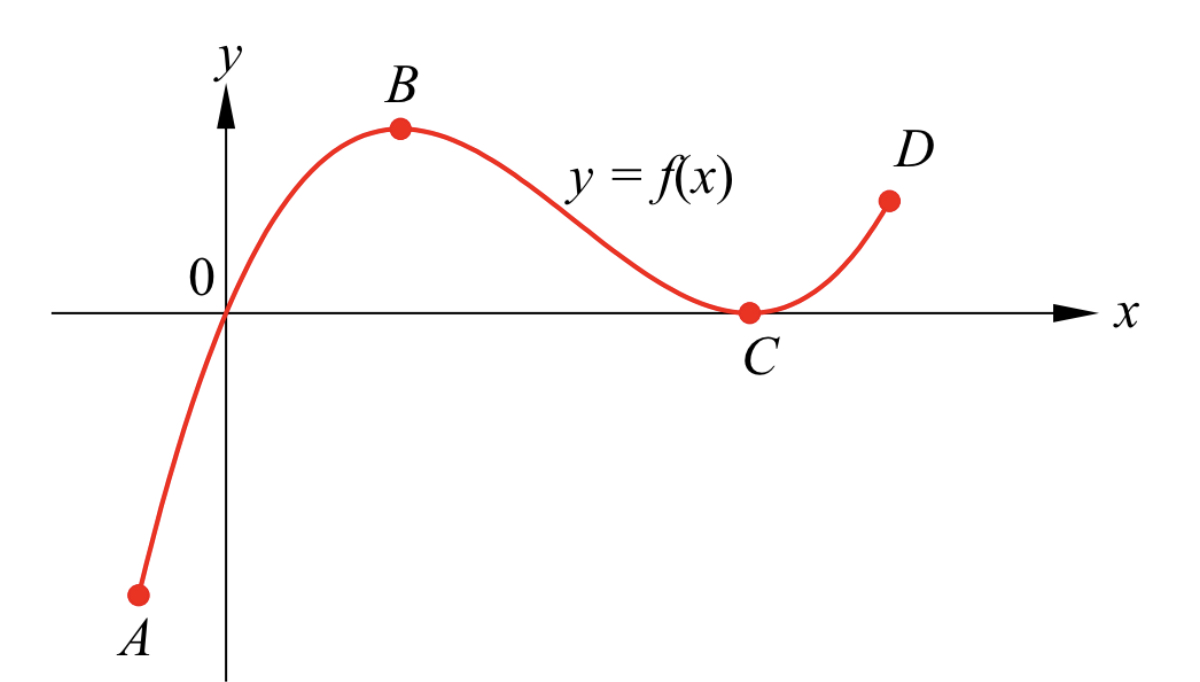
\includegraphics[scale=0.2]{Picture22.png}
\caption{  The function $y=f(x)$ has local maxima at the points $B$ and $D$, and local minima at the points $A$ and $C$. The point $A$ is also where global minimum appears; while the point $B$ is where the global maximum appears.\fa}\label{figure22}
\end{figure}

Derivative is an useful tool in the search for local extrema. 
When a local extremizer of a function is an interior point of the domain, and $f$ is differentiable at that point, the derivative of the function can only be zero at that point.
\begin{theorem}[label=thm230215_2]{}
Let $(a, b)$ be a neighbourhood of the point $x_0$, and let $f:(a,b)\to\mathbb{R}$ be a function defined on $(a,b)$. If $x_0$ is a local extremizer of $f$, and $f$ is differentiable at $x_0$, then $f'(x_0)=0$.
\end{theorem}
\begin{myproof}{Proof}Without loss of generality, assume that $x_0$ is a local maximizer. Then there is a $\delta>0$ such that $(x_0-\delta, x_0+\delta)\subset (a,b)$, and for all $x$ in $(x_0-\delta, x_0+\delta)$, $f(x)\leq f(x_0)$. 
Since $f$ is differentiable at $x_0$, the limit
\[\lim_{x\to x_0}\frac{f(x)-f(x_0)}{x-x_0}\] exists and is equal to $f'(x_0)$. This implies that the left limit and the right limit both exist and both equal to $f'(x_0)$.
Namely,
\[f'(x_0)=\lim_{x\to x_0^-}\frac{f(x)-f(x_0)}{x-x_0}=\lim_{x\to x_0^+}\frac{f(x)-f(x_0)}{x-x_0}.\]\bp
For the left limit, when $x$ is in $(x_0-\delta, x_0)$, $x-x_0<0$ and $f(x)-f(x_0)\leq 0$. Therefore,
\[\frac{f(x)-f(x_0)}{x-x_0}\geq 0\hspace{1cm}\text{when}\;x\in (x_0-\delta, x_0).\]
Taking the $x\to x_0^-$ limit, we find that $f'(x_0)\geq 0$. For the right limit, when $x$ is in $(x_0, x_0+\delta)$, $x-x_0>0$ but $f(x)-f(x_0)\leq 0$.  Therefore,
\[\frac{f(x)-f(x_0)}{x-x_0}\leq 0\hspace{1cm}\text{when}\;x\in (x_0, x_0+\delta).\]
Taking the $x\to x_0^+$ limit, we find that $f'(x_0)\leq 0$. Since the left limit shows that $f'(x_0)\geq 0$ while the right limit shows that $f'(x_0)\leq 0$,  we conclude that $f'(x_0)=0$.
\end{myproof}
This theorem gives a necessary condition for a function $f:(a,b)\rightarrow\mathbb{R}$ to have a local extremum at a point where it is differentiable. Notice that it cannot be applied if the local extremizer is not an interior point of the domain. 

\begin{definition}{Stationary Points}
Let $D$ be a subset of real numbers and let $f:D\to\mathbb{R}$ be a function defined on $D$. If $x_0$ is an interior point of $D$,   $f$ is differentiable at $x_0$ and $f'(x_0)=0$, we call $x_0$ a stationary point of the function $f$. 
\end{definition}

Hence, Theorem \ref{thm230215_2} says that if $x_0$ is an interior point of $D$, and the function $f:D\to\mathbb{R}$ is differentiable at $x_0$, a necessary condition for $x_0$ to be a local extremum of the function $f$ is $x_0$ must be a stationary point.
Nevertheless, this condition is not sufficient. For example, the function $f(x)=x^3$ has a stationary point at $x=0$, but $x=0$ is not a local extremizer of the funnction.

Now let us return to the mean value theorem. 
As a motivation, let us consider the distance $s$ travelled by an object as a function of time $t$. We have discussed in Section \ref{sec3.1} that to find the instantaneous speed of the object at a particular time $t_0$, we first find the average speed over the time interval from $t_0$ to $t_0+\Delta t$, and take the limit  $\Delta t\to 0$. Namely, the instantaneous speed at time $t_0$ is
\[\lim_{\Delta t\to 0}\frac{s(t_0+\Delta t)-s(t_0)}{\Delta t},\] which is precisely $s'(t_0)$, the derivative of $s(t)$ at $t=t_0$. The mean value theorem asserts that the average speed of the object in a time interval $[t_1, t_2]$ must equal to the instantaneous speed $s'(t_0)$ for some $t_0$ in that interval. Intuitively, this is something one would expect to be true.

Now let us prove a special case of the mean value theorem.
\begin{theorem}[label=thm_Rolles]{Rolle's Theorem}
Let $f:[a,b]\to\mathbb{R}$ be a function that satisfies the following conditions.
\begin{enumerate}[(i)]
\item $f:[a,b]\to\mathbb{R}$ is continuous.
\item $f:(a, b)\to\mathbb{R}$ is differentiable.
\item $f(a)=f(b)$.
\end{enumerate}
Then there is a point $x_0$ in $(a, b)$ such that $f'(x_0)=0$. 
\end{theorem}
\begin{myproof}{Proof}
Since $f:[a,b]\to\mathbb{R}$ is a continuous function defined on a closed and bounded interval, the extreme value theorem says that it must have minimum value and maximum value. In other words, there are two points $x_1$ and $x_2$ in  $[a,b]$ such that
\[f(x_1)\leq f(x)\leq f(x_2)\hspace{1cm}\text{for all}\;x\in [a,b].\] Notice that $x_1$ and $x_2$ are also local extremizers of the function $f:[a,b]\to\mathbb{R}$.
If $f(x_1)=f(x_2)$, then $f$ is a constant function. In this case,  $f'(x_0)=0$ for all $x_0$ in $(a, b)$.
If $f(x_1)\neq f(x_2)$, then $f(x_1)<f(x_2)$. Since $f(a)=f(b)$, either $x_1$ or $x_2$ must be in the open interval $(a, b)$. In other words, there is a local extremizer $x_0$ in the interval $(a,b)$. Since $f$ is differentiable at $x_0$, Theorem \ref{thm230215_2}  says that we must have $f'(x_0)=0$.
In either case,   there is an $x_0$ in $(a, b)$ satisfying $f'(x_0)=0$.
\end{myproof}


 \begin{figure}[ht]
\centering
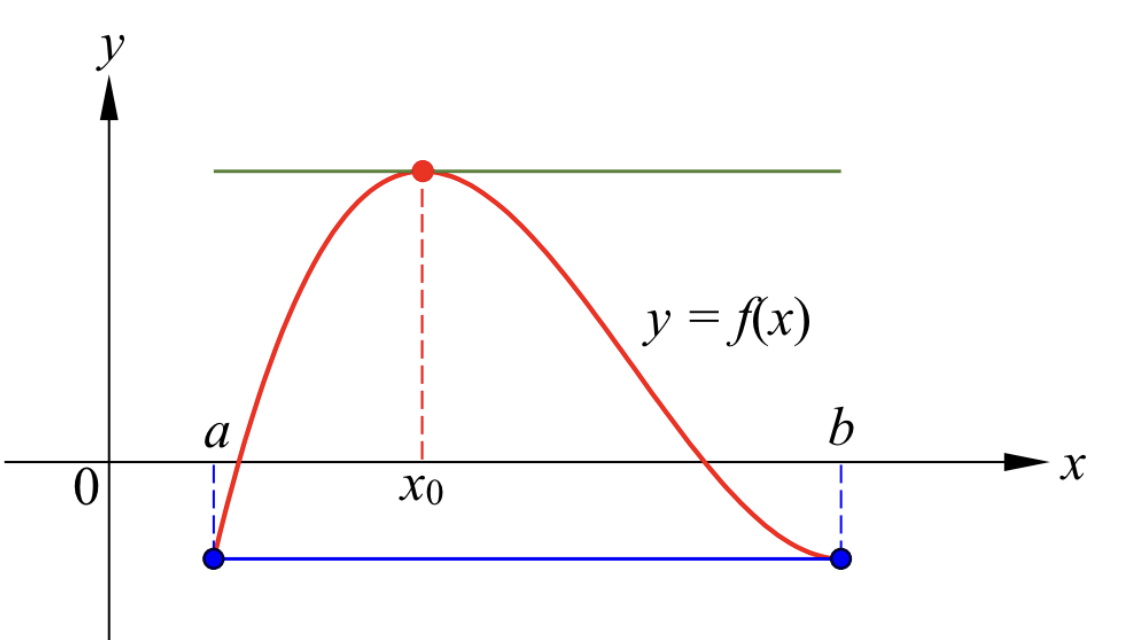
\includegraphics[scale=0.2]{Picture23.png}
\caption{  The Rolle's theorem.\fa}\label{figure23}
\end{figure}

Now we can prove the mean value theorem.
\begin{theorem}[label=thm_mvt]{Mean Value Theorem}
Let $f:[a,b]\to\mathbb{R}$ be a function that satisfies the following conditions.
\begin{enumerate}[(i)]
\item $f:[a,b]\to\mathbb{R}$ is continuous.
\item $f:(a, b)\to\mathbb{R}$ is differentiable.
 
\end{enumerate}
Then there is a point $x_0$ in $(a, b)$ such that \[f'(x_0)=\frac{f(b)-f(a)}{b-a}.\]
\end{theorem}
The mean value theorem stated in Theorem \ref{thm_mvt} is also referred to as Lagrange's mean value theorem.
Notice that Rolle's theorem is a special case of the mean value theorem where $f(a)=f(b)$. The quantity 
\[\frac{f(b)-f(a)}{b-a}\] gives the average rate of change of the function $f(x)$ over the interval $[a, b]$, and the mean value theorem says that this average rate of change is equal to the rate of change at a particular point. To prove the mean value theorem, we apply a transformation to the function $f(x)$ to get a function $g(x)$ that satisfies the conditions in the Rolle's theorem.  
\begin{myproof}{Proof}
Let $g:[a,b]\to\mathbb{R}$ be the function defined by \[g(x)= f(x)-mx,\]
where the constant $m$ is determined by $g(a)=g(b)$.
This gives
\[f(a)-ma=f(b)-mb,\]
and so
\[m=\frac{f(b)-f(a)}{b-a}.\]Notice that the function $g:[a,b]\to\mathbb{R}$ is continuous, and $g:(a, b)\to \mathbb{R}$ is differentiable with
\[g'(x)=f'(x)-m=f'(x)-\frac{f(b)-f(a)}{b-a}.\]
By construction, $g(a)=g(b)$. Hence, we can apply Rolle's theorem to the function $g$ and conclude that there is a point $x_0$ in $(a,b)$ such that $g'(x_0)=0$. For this point $x_0$,
\[f'(x_0)=\frac{f(b)-f(a)}{b-a}.\]This proves the mean value theorem.
\end{myproof}


 \begin{figure}[ht]
\centering
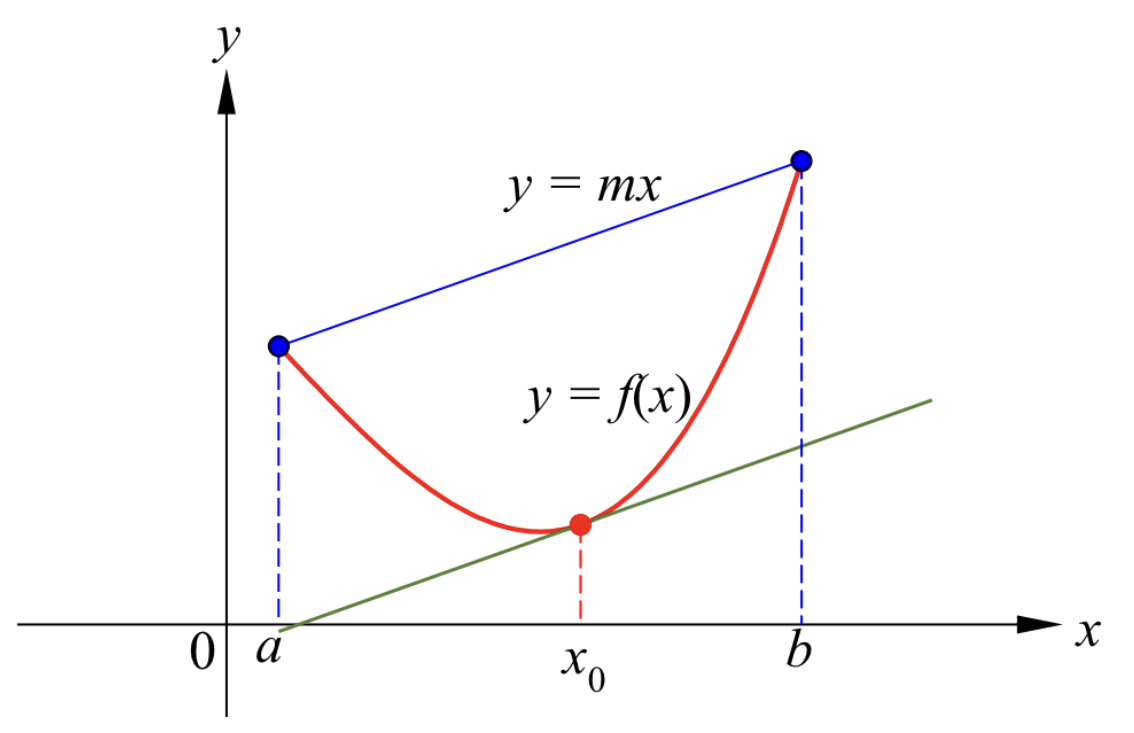
\includegraphics[scale=0.2]{Picture24.png}
\caption{  The mean value theorem.\fa}\label{figure24}
\end{figure}
Notice that for the mean value theorem to hold, the function $f:[a,b]\to\mathbb{R}$ do not need to be differentiable at the end points of the interval $[a,b]$, and the point $x_0$ is guaranteed to be a point in the interior of the interval. 

The mean value theorem has very wide applications. We will discuss a few in this section.  



Recall that the derivative of a constant function is 0. The converse is not obvious, but it is an easy consequence of the mean value theorem.
\begin{lemma}[label=lemma230215_2]{}
If the function $f:[a,b]\to\mathbb{R}$ is continuous on $[a, b]$, differentiable on $(a,b)$, and $f'(x)=0$ for all $x\in (a,b)$, then $f$ is a constant function.
\end{lemma}
\begin{myproof}{}
Take any $x\in (a, b]$. Then $f$ is continuous on $[a, x]$, differentiable an $(a, x)$. Therefore, we can apply mean value theorem to conclude that there is a point $c$ in $(a, x)$  such that
\[\frac{f(x)-f(a)}{x-a}=f'(c)=0.\]
This proves that $f(x)=f(a)$. Therefore, the function $f$ is a constant.
\end{myproof}

From this, we immediately obtain the following.
\begin{theorem}[label=thm230215_3]{ }
Assume that the functions $f:[a,b]\to\mathbb{R}$ and $g:[a,b]\to\mathbb{R}$ are continuous on $[a,b]$, differentiable on $(a,b)$, and 
\[f'(x)=g'(x)\hspace{1cm}\text{for all}\;x\in (a,b).\]
Then there is a constant $C$ such that
\[f(x)=g(x)+C\hspace{1cm}\text{for all}\; x\in [a,b].\]
\end{theorem}
\begin{myproof}{Proof}
Define the function $h:[a,b]\to\mathbb{R}$ by
\[h(x)=f(x)-g(x).\] Then the function $h$ is continuous on $[a, b]$, differentiable on $(a,b)$, and $h'(x)=0$ for all $x\in (a,b)$. By Lemma \ref{lemma230215_2}, $h$ is a cosntant function. Namely, there is a constant $C$ so that $h(x)=C$ for all $x\in [a, b]$. Therefore,
\[f(x)=g(x)+C\hspace{1cm}\text{for all}\; x\in [a,b].\]
\end{myproof}

\begin{highlight}{}
Theorem \ref{thm230215_3} implies   \emph{the identity criterion}, which says that if two  functions are differentiable in an open interval, their derivatives are the same, and their values at a single point in the interval coincide, then these two functions must be identical.
\end{highlight}

We have seen that if $p(x)$ is a polynomial of degree $n$, and $k$ is an integer larger than $n$, then the $k^{\text{th}}$-order derivative of $p(x)$ is identically zero. Using Lemma \ref{lemma230215_2}, we can prove that the converse is also true.

\begin{example}{}
Let $n$ be a nonnegative integer. Assume that the function $p:\mathbb{R}\to\mathbb{R}$ is $(n+1)$ times differentiable and $p^{(n+1)}(x)=0$ for all real numbers $x$. Then $p(x)$ is a polynomial of degree at most $n$.
\end{example}
\begin{myproof}{Proof}
We prove this by induction on $n$. When $n=0$, the statement says that if $p:\mathbb{R}\to\mathbb{R}$ is a differentiable function and $p'(x)=0$ for all $x\in\mathbb{R}$, then $p(x)$ is a polynomial of degree  0. Since a polynomial of degree 0 is a constant, this statement is true by Lemma \ref{lemma230215_2}.

Now let $n\geq 1$, and assume that
 we have proved that for any $k<n$, if $q:\mathbb{R}\to\mathbb{R}$ is a function that is $(k+1)$ times differentiable and $q^{(k+1)}(x)=0$ for all real numbers $x$, then $q(x)$ is a polynomial of degree at most $k$. \bp Let $p:\mathbb{R}\to\mathbb{R}$ be a function that is $(n+1)$ times differentiable and $p^{(n+1)}(x)=0$ for all real numbers $x$. Lemma \ref{lemma230215_2} says that there is a constant $C$ such that
\[p^{(n)}(x)=C.\]
Consider the function $q:\mathbb{R}\to\mathbb{R}$ defined by
\[q(x)=p(x)-\frac{C}{n!}x^n.\]
It is $n$ times differentiable and
\[q^{(n)}(x)=p^{(n)}(x)-C=0\hspace{1cm}\text{for all}\;x\in\mathbb{R}.\]
By inductive hypothesis,
$q(x)$ is a polynomial of degree at most $n-1$. Namely, there are constants $a_0$, $a_1$, $\ldots$, $a_{n-1}$ such that
\[q(x)=a_{n-1}x^{n-1}+\cdots+a_1 x+a_0.\]
This implies that
\[p(x)=a_nx^n+a_{n-1}x^{n-1}+\cdots+a_1x+a_0,\]where $a_n=C/n!$. Hence, $p(x)$ is a polynomial of degree at most $n$.
\end{myproof}






Mean value theorem can be used to estimate the magnitude of a function provided that we know the derivative.
\begin{example}{}
Given that the function $f:[0,10]\to\mathbb{R}$ is continuous on $[0,10]$, differentiable on $(0,10)$, and $-3<f'(x)<8$ for all $x$ in $ (0,10)$. If $f(0)=-2$, find a range for the values of $f(x)$.
\end{example}
\begin{solution}{Solution}
Let $x$ be point in  $(0, 10]$. By mean value theorem, there is a $c\in (0, x)$ such that
\[\frac{f(x)-f(0)}{x-0}=f'(c).\]
Since $-3<f'(c)<8$, we find that
\[-3x<f(x)+2<8x.\]
This implies that
\[ -32<-3x-2<f(x)<8x-2<78.\]Therefore, a range for the values of $f(x)$ is $(-32, 78)$.
\end{solution}

The next example shows that the mean value theorem can be used to determine the number of solutions of an equation.
\begin{example}{}
Recall that in Example \ref{ex230215_1}, we have shown that the equation 
\[x^6+6x+1=0\]has a real root. Determine the exact number of real roots of this equation.


\end{example}
\begin{solution}{Solution}
Let $f:\mathbb{R}\to\mathbb{R}$ be the function $f(x)=x^6+6x+1$. This is a  differentiable function with\[f'(x)=6x^5+6.\]From this, we find that $f'(x)=0$ if only if $x^5=-1$, if and only if $x=-1$.   

If $x_1$ and $x_2$ are two points such that $x_1<x_2$ and $f(x_1)=f(x_2)=0$,  Rolle's theorem says that there is a point  $u$ in $(x_1, x_2)$  such that $f'(u)=0$. 

\bs
If $f(x)=0$ has three distinct real roots, we can assume that these real roots are $x_1$, $x_2$ and $x_3$ with $x_1<x_2<x_3$. Then there is a $u_1$ in $(x_1, x_2)$, and a $u_2$ in $(x_2, x_3)$ such that  
$f'(u_1)=f'(u_2)=0$. In other words, $f'(x)=0$ has two distinct real  roots $u_1$ and $u_2$. But we have shown that there is only one $x$ such that $f'(x)=0$. Therefore, $f(x)=0$ can have at most two real solutions.

Since $f(0)=1$, we have $f(-1)<0<f(1)$. By intermediate value theorem, there is a $c_1\in (-1, 0)$ such that $f(c_1)=0$.

Since $f(-2)=53$, we have $f(-1)<0<f(-2)$. By intermediate value theorem, there is a $c_2\in (-2, -1)$ such that $f(c_2)=0$. 

We conclude that $f(x)=0$ has exactly two real roots.




\end{solution}
Another important application of the mean value theorem is to determine the increasing or decreasing patterns of functions.

\begin{theorem}[label=thm230215_4]{}
Given that $f:[a,b]\to\mathbb{R}$ is a function continuous on $[a,b]$, and differentiable on $(a, b)$.
\begin{enumerate}[1.]
\item If $f'(x)>0$ for all $x\in (a, b)$, then $f:[a,b]\to\mathbb{R}$ is a strictly increasing function.
\item If $f'(x)<0$ for all $x\in (a, b)$, then $f:[a,b]\to\mathbb{R}$ is a strictly decreasing function.
\end{enumerate}
\end{theorem}
Notice that we only assume that $f'$ is positive or negative on the open interval $(a, b)$. If $f'$ exists at the end points, it can be 0 there, and the conclusion about the strict monotonicity still holds for the entire closed interval $[a,b]$.
\begin{myproof}{Proof}
It suffices for us to prove the first statement. Given any two points $x_1$ and $x_2$ in the closed interval $[a,b]$ with $x_1<x_2$, the function $f$ is continuous on $[x_1, x_2]$, differentiable on $(x_1, x_2)$, and $f'(x)>0$ for any $x\in (x_1, x_2)$. By mean value theorem, there is a point $c$ in $(x_1, x_2)$ such that \bp
\[\frac{f(x_2)-f(x_1)}{x_2-x_1}=f'(c).\]  Since $f'(c)>0$ and $x_2-x_1>0$, we conclude that
\[f(x_2)>f(x_1).\]
This proves that $f:[a,b]\to\mathbb{R}$ is  strictly increasing.
\end{myproof}

We look at a simple example.
\begin{example}[label=ex230216_8]{}
Consider the function $f:\mathbb{R}\to\mathbb{R}$, $f(x)=x^3$. Notice that $f$ is differentiable and $f'(x)=3x^2$. Hence, $f'(x)>0$ for $x\neq 0$, but $f'(0)=0$. Therefore, we cannot apply Theorem \ref{thm230215_4} directly to conclude that $f:\mathbb{R}\to\mathbb{R}$, $f(x)=x^3$ is a strictly increasing function. However, we can proceed in the following way. Since $f'(x)>0$ on the open interval $(-\infty, 0)$, Theorem \ref{thm230215_4} implies that $f$ is strictly increasing on the closed interval $(-\infty, 0]$. Since  $f'(x)>0$ on the open interval $(0, \infty)$, Theorem \ref{thm230215_4} again implies that $f$ is strictly increasing on the closed interval $[0, \infty)$. Combining together, we conclude that  $f:\mathbb{R}\to\mathbb{R}$, $f(x)=x^3$ is strictly increasing.
\end{example}

\begin{remark}{}
Let   $f:[a, b]\to\mathbb{R}$ be a function defined on $[a, b]$, and let $x_1, \ldots, x_n$ be points in $(a, b)$ such that the following conditions are satisfied.
\begin{enumerate}[(i)]
\item $f$ is  continuous on $[a,b]$, differentiable on $(a, b)$.
\item   $f'(x_k)=0$ for $1\leq k\leq n$.
\item $f'(x)>0$ for any $x\in (a, b)\setminus\{x_1, \ldots, x_n\}$.
\end{enumerate}
Using the same reasoning as in Example \ref{ex230216_8},  one can prove that $f$ is strictly increasing on $[a, b]$.
\end{remark}

Example \ref{ex230216_8} shows that if a function $f:(a, b)\to\mathbb{R}$ is differentiable and strictly increasing, it is not necessary that $f'(x)>0$ for all $x\in (a, b)$. If we relax the strict monotonicity to  monotonicity,  we will find that $f'(x)\geq 0$ for all $x\in (a, b)$ is sufficient and necessary for $f$ to be increasing.

\begin{theorem}[label=thm230216_9]{}
Given that the function $f:[a,b]\to\mathbb{R}$ is  continuous on $[a,b]$, and differentiable on $(a, b)$.
\begin{enumerate}[1.]
\item $f:[a,b]\to\mathbb{R}$ is an  increasing function if and only if   $f'(x)\geq 0$ for all $x\in (a, b)$.
\item $f:[a,b]\to\mathbb{R}$ is a decreasing function if and only if   $f'(x)\leq 0$ for all $x\in (a, b)$.
\end{enumerate}
\end{theorem}
\begin{myproof}{Proof} Again, let us consider the first statement. 
If $f'(x)\geq 0$ for all $x\in (a,b)$,  the proof that $f$ is increasing is almost verbatim the proof in Theorem \ref{thm230215_4}, with $>$ replaced by $\geq $. For the converse, if $f$ is increasing on $[a, b]$, we want to show that $f'(x_0)\geq 0$ for any $x_0$ in $(a, b)$. This follows from the fact that
\[\frac{f(x)-f(x_0)}{x-x_0}\geq 0\] for any $x$ in $(a, b)\setminus\{0\}$ since $f$ is increasing. Taking limit gives $f'(x_0)\geq 0$.
\end{myproof}

For a   function $f(x)$ that is differentiable,  the condition $f'(x_0)=0$ is   necessary  for an interior point $x_0$ to be a local extremizer, but not sufficient.
Theorem  \ref{thm230215_4} provides the tool  for determining whether such point is a local extremizer. It is called the \emph{first derivative test}. We would not go into the general formulation. Instead, we will apply Theorem  \ref{thm230215_4} or Theorem \ref{thm230216_9} directly to solve such problems.

\begin{example}[label=ex230216_1]{}
Consider the function $f:\mathbb{R}\to\mathbb{R}$ defined by
\[f(x)=\frac{x}{x^2+1}.\]
Find the local maximum value and the local minimum value of $f$, and find the range of the function $f$. 
 
\end{example}
\begin{solution}{Solution}
Since $f$ is a rational function, it is differentiable, and
\[f'(x)=\frac{(x^2+1)-x(2x)}{(x^2+1)^2}=\frac{1-x^2}{(x^2+1)^2}=-\frac{(x+1)(x-1)}{(x^2+1)^2}.\]Since $f$ is differentiable everywhere, the only candidates for the local maximizer and the local minimizer are those points $x$ where $f'(x)=0$, which are the poins $x=-1$ and $x=1$.
\begin{enumerate}[$\bullet$\;\;]
\item
 When $x\in (-\infty, -1)$, $f'(x)<0$,  and so $f$ is   decreasing on $(-\infty, 1]$. 
\item When $x\in (-1, 1)$, $f'(x)>0$,  and so $f$ is   increasing on $[-1, 1]$. 
\item When $x\in (1, \infty)$, $f'(x)<0$,  and so $f$ is   decreasing on $[1, \infty)$. 
\end{enumerate}These imply that $x=-1$ is a local minimizer, and   $x=1$ is a local maximizer. 
The local maximum value of $f$ is $f(1)=\frac{1}{2}$, and the local minimum value is $f(-1)=-\frac{1}{2}$.
Notice that
\[\lim_{x\to -\infty}f(x)=\lim_{x\to\infty} f(x)=0.\]Since $f$ is   decreasing on $(-\infty, -1]$,   for any $x$ in $(-\infty, -1]$, \[-\frac{1}{2}=f(-1)\leq f(x)<0.\]
Since $f$ is   increasing on $[-1, 1]$, for any $x$ in $[-1, 1]$, 
\[-\frac{1}{2}=f(-1)\leq f(x)\leq f(1)=\frac{1}{2}.\]
\bs Since $f$ is decreasing   on $[1, \infty)$,  for any $x$ in $[1, \infty)$, \[0<f(x)\leq f(1)=\frac{1}{2}.\]
Combining together, we conclude that the range of $f$ is $[-\frac{1}{2}, \frac{1}{2}]$.
 
\end{solution}


 \begin{figure}[ht]
\centering
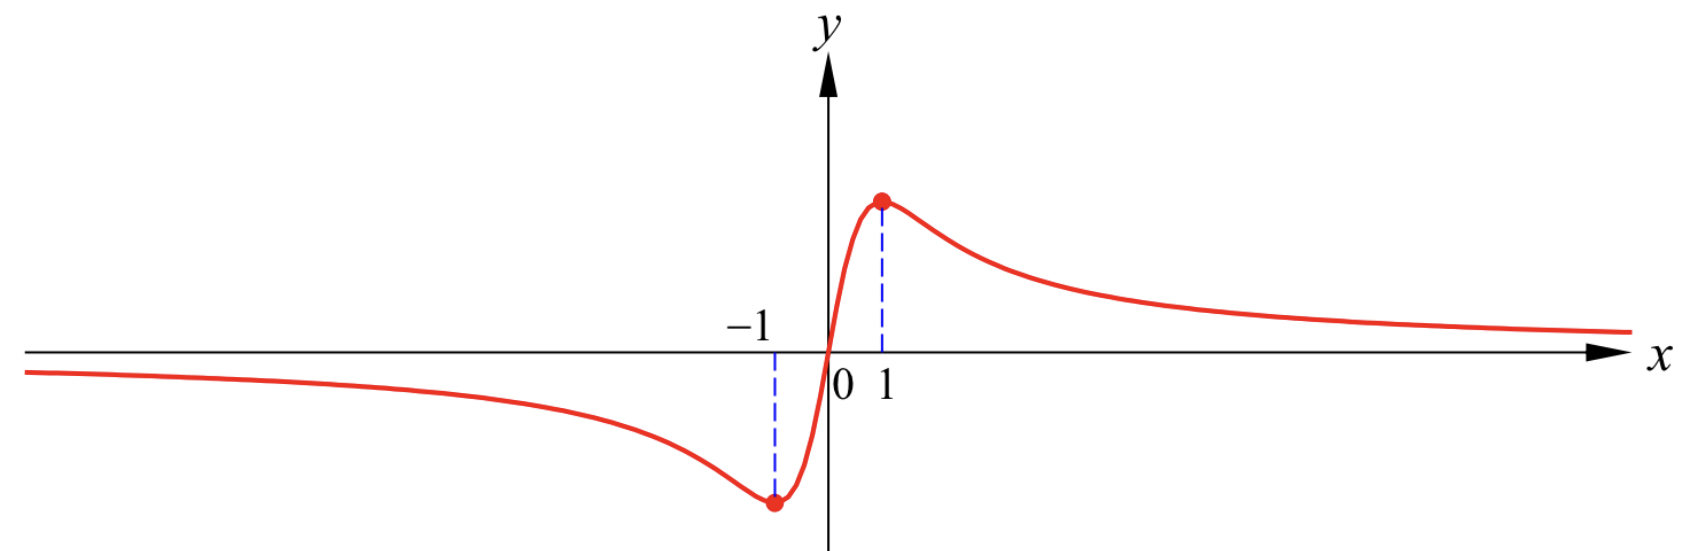
\includegraphics[scale=0.2]{Picture25.png}
\caption{  The function $\di f(x)=\frac{x}{x^2+1}$.\fa}\label{figure25}
\end{figure}

There is also a \emph{second derivative test} for determining whether a stationary point is a local minimizer or a local maximizer.

\begin{theorem}[label=thm230215_6]{Second Derivative Test}
Let $(a,b)$ be an interval that contains the point $x_0$, and let $f:(a, b)\to\mathbb{R}$ be a  differentiable function. Assume that $f'(x_0)=0$, and $f''(x_0)$ exists.
\begin{enumerate}[1.]
\item
If $f''(x_0)>0$, then $x_0$ is a local minimizer of $f$.
\item If $f''(x_0)<0$, then $x_0$ is a local maximizer of $f$.
\end{enumerate}
\end{theorem}

\begin{highlight}{}The second derivative test is inconclusive  if $f''(x_0)=0$, as can be shown by considering the three functions $f_1(x)=x^4$, $f_2(x)=-x^4$ and $f_3(x)=x^3$. All these three functions have $x=0$ as  a stationary point. Their second derivatives are all equal to zero at $x=0$. However, $x=0$ is a local minimizer of $f_1(x)=x^4$, it is a local maximizer of the function $f_2(x)=-x^4$, and it is not a local extremizer for the function $f_3(x)=x^3$.\end{highlight}

\begin{myproof}{\linkt Proof of Theorem \ref{thm230215_6}}
We will give a proof of the first statement. The proof of the second statement is similar.
For the first statement, we are given that $f'(x_0)=0$ and $f''(x_0)>0$. By definition, 
\[f''(x_0)=\lim_{x\to x_0}\frac{f'(x)-f'(x_0)}{x-x_0}=\lim_{x\to x_0}\frac{f'(x)}{x-x_0}.\]
Take $\varepsilon$ to be the positive number $f''(x_0)/2$. The definition of limit implies that there is a $\delta>0$ such that $(x_0-\delta, x_0+\delta)\subset (a, b)$, and for all the points $x$ in $(x_0-\delta, x_0)\cup (x_0, x_0+\delta)$, 
\[\left|\frac{f'(x)}{x-x_0}-f''(x_0)\right|<\frac{f''(x_0)}{2}.\]
This implies that for all $x\in (x_0-\delta, x_0)\cup (x_0, x_0+\delta)$,
\begin{equation}\label{eq230215_7}\frac{f'(x)}{x-x_0}>f''(x_0)-\frac{f''(x_0)}{2}=\frac{f''(x_0)}{2}>0.\end{equation}

If $x\in (x_0-\delta, x_0)$, $x-x_0<0$. Equation \eqref{eq230215_7} implies that $f'(x)<0$. Therefore, $f$ is   decreasing on $(x_0-\delta, x_0]$. This implies that
\[f(x)\geq f(x_0)\hspace{1cm} \text{for all}\;x\in (x_0-\delta, x_0).\]
If $x\in (x_0, x_0+\delta)$, $x-x_0>0$. Equation \eqref{eq230215_7} implies that $f'(x)>0$. Therefore, $f$ is   increasing on $[x_0, x_0+\delta)$. This implies that
\[f(x)\geq f(x_0)\hspace{1cm} \text{for all}\;x\in (x_0, x_0+\delta).\]
Combining together, we find that $f(x)\geq f(x_0)$ for all $x$ in $(x_0-\delta, x_0+\delta)$. This proves that $x_0$ is a local minimizer of $f$.


\end{myproof}
 
\begin{example}{}
For the function $\di f(x)$ considered in Example \ref{ex230216_1}, we have shown that the stationary points are $x=-1$ and $x=1$. A tedious computation gives
\[f''(x)=\frac{2x(x^2-3)}{(x^2+1)^3}.\]
Hence,
\[f''(-1)=\frac{1}{2},\hspace{1cm}f''(1)=-\frac{1}{2}.\]The second derivative test can then be used to conclude that
$x=-1$ is a local minimizer, and $x=1$ is a local maximizer.
\end{example}
Although applying the second derivative test seems straightforward, an analysis using the first derivative test is more conclusive. Finding the second derivative can also be tedious, as shown in the example above.

At the end of this section, we want to prove an analogue of intermediate value theorem for derivatives.
\begin{theorem}{Darboux's Theorem}
Let $f:[a,b]\to\mathbb{R}$ be a differentiable function. If $w$ is a value strictly between $f_+'(a)$ and $f_-'(b)$, then there is a point $c$ in $(a, b)$ such that
$f'(c)=w$.
\end{theorem}If the function $g'$ is continuous, then Darboux's theorem follows immediately from the intermediate value theorem. The strength of Darboux's theorem lies in the fact that it does not     assume the continuity of $g'$. 

\begin{myproof}{Proof} The proof   is an again an application of the extreme value theorem.

 Without loss of generality,   assume that $f_+'(a)<w<f_-'(b)$. 
Since $f:[a,b]\to\mathbb{R}$ is a differentiable function, it is continuous. 
Define the function $g:[a,b]\to\mathbb{R}$ by
\[g(x)=f(x)-wx.\]\bp
Then $g$ is differentiable and
\[g'(x)=f'(x)-w.\]
Notice that $g:[a,b]\to\mathbb{R}$ is also continuous. By extreme value theorem, $g:[a,b]\to\mathbb{R}$ has a  minimum value. Now,
\[g'_+(a)=f_+'(a)-w<0,\hspace{1cm} g_-'(b)=f_-'(b)-w>0.\]
 By definition,
\[g_+'(a)=\lim_{x\to a^+}\frac{g(x)-g(a)}{x-a}.\] Taking $\varepsilon$ to be the positive number $-g_+'(a)/2$, we find that there is a $\delta>0$ such that $\delta\leq b-a$, and for all $x\in (a, a+\delta)$,  
\[\frac{g(x)-g(a)}{x-a}<g_+'(a)+\varepsilon= \frac{g_+'(a)}{2}<0.\]In particular, for all $x\in (a, a+\delta)$, $g(x)<g(a)$, and thus $g(a)$ is not a minimum value of the function $g$. Similarly, since $g_-'(b)>0$, we find that $g(b)$ is not a minimum value of the function $g$. In other words, the minimizer of $g$ must be a point $c$ inside $(a, b)$. This is then also a local minimizer. Since $g$ is differentiable, we must have $g'(c)=0$. This implies that $f'(c)=w$.

\end{myproof}

\begin{remark}[label=remark230216_1]{}
As a consequence of the Darboux's theorem, we find that if a function $f:(a,b)\to\mathbb{R}$ is differentiable and $f'(x)\neq 0$ for any $x\in (a, b)$, then either $f'(x)>0$ for all $x\in (a, b)$, or $f'(x)<0$ for all $x\in (a, b)$. In any case, this means that such  a function must be strictly monotonic. 
\end{remark}

Before closing this section, let us define a terminology.
\begin{definition}{$\pmb{C^k}$ functions}
Let $k$ be a nonnegative integer.
We say that a function $f:(a, b)\to\mathbb{R}$ is a $C^k$-function it is has $k$ times derivatives and the $k^{\text{th}}$-derivative $f^{(k)}:(a,b)\to\mathbb{R}$ is also continuous. 
\end{definition}
It s easy to see that if  $f:(a, b)\to\mathbb{R}$ is a $C^k$-function, then for any $0\leq j<k$, $f^{(j)}:(a,b)\to\mathbb{R}$ is   continuous. 

A $C^0$ function is just a continuous function.
A $C^1$ function is   called a continuously differentiable function.
In general, a $C^k$ function is called a $k$-times continuously differentiable function.

The definition of $C^k$ functions can be extended to the case where the function $f$ is defined on a closed interval $[a, b]$.
\vp
\noindent
{\bf \large Exercises  \thesection}
\setcounter{myquestion}{1}

\begin{question}{\themyquestion}
Given that the function $f:[-5,8]\to\mathbb{R}$ is continuous on $[-5,8]$, differentiable on $(-5,8)$, and $-4<f'(x)<4$ for all $x$ in $ (-5,8)$. If $f(0)=2$, find a range for the values of $f(x)$.
\end{question}

\atc
\begin{question}{\themyquestion}
Show that the function $f:\mathbb{R}\to\mathbb{R}$, 
\[f(x)=\frac{x^3}{x^2+1}\]
is strictly increasing, and find the range of the function.

\end{question}
\atc
\begin{question}{\themyquestion}
Show that the equation
\[ x^5+x+32=0\] has exactly one real solution.
\end{question}
\atc
\begin{question}{\themyquestion}
Find the number of real solutions of the equation
\[ \frac{32x}{x^4+16}=1.\]
\end{question}
\atc
\begin{question}{\themyquestion}
Let $n$ be a nonnegative integer, and let $f:(a, b)\to\mathbb{R}$ be a differentiable function.  If the equation $f'(x)=0$ has   $n$ distinct real roots in the interval $(a,b)$, show that the equation $f(x)=0$ has at most $(n+1)$ distinct real roots in the interval $(a, b)$.
\end{question}
 
\atc
\begin{question}{\themyquestion}
Consider the function $f:\mathbb{R}\to\mathbb{R}$ defined by
\[f(x)=\frac{x+1}{x^2+15}.\]
\begin{enumerate}[(a)]
\item 
Find the local maximum value and the local minimum value of $f$.
\item Find the range of the function $f$. 
\end{enumerate}
\end{question}

\atc
\begin{question}{\themyquestion}
Let $f:[a, b]\to \mathbb{R}$ be a function such that the limit 
\[L=\lim_{x\to b^-}\frac{f(x)-f(b)}{x-b} \]
 exists. If $L>0$, show that there is a $\delta>0$ such that $\delta\leq b-a$ and for all $x\in (b-\delta, b)$,
\[f(x)<f(b).\]

\end{question}

\atc
\begin{question}{\themyquestion}
Let $f:(a, b)\to \mathbb{R}$ be a differentiable function. Suppose that $f':(a,b)\to\mathbb{R}$ is monotonic, show that $f':(a,b)\to\mathbb{R}$ is continuous.

\end{question}
\vp
\section{The Cauchy Mean Value Theorem}\label{sec3.4}
In previous section, we have seen that the mean value theorem is very useful in analysing the behavior of a differentiable function. For future applications, we will often quote it in the following form.
\begin{highlight}{Alternative Form of Mean Value Theorem} If $f:(a, b)\to \mathbb{R}$ is a differentiable function, $x_0$ is a point in $(a, b)$, $h$ is such that $x_0+h$ is also in $(a, b)$, then there is a number $c\in (0,1)$ such that 
\begin{equation}\label{eq230216_3}f(x_0+h)-f(x_0)=f'(x_0+ch)h.\end{equation}
\end{highlight}
To see this, let $x_1=x_0+h$.  If $h=0$, \eqref{eq230216_3} is obviously true for any $c$ in $(0, 1)$. If $h\neq 0$, then when $c$ runs through all values from 0 to 1, $x_0+ch$ runs through all points in the open interval  $I$ with $x_0$ and $x_1$ as endpoints. Thus, \eqref{eq230216_3} says that
\[ f(x_1)-f(x_0)=f'(u)(x_1-x_0)\] for some $u$ in the open intefval $I$, which is precisely the statement of the mean value theorem.

When finding limits of functions, we often encounter situations like
\[\lim_{x\to x_0}\frac{f(x)}{g(x)}\] where both $\di\lim_{x\to x_0}f(x)$ and $\di\lim_{x\to x_0}g(x)$ are   zero. For example, let  \[f(x)=x^{20}+2x^9-3\hspace{1cm}\text{and} \hspace{1cm} g(x)=x^7-1.\] Then \[\lim_{x\to 1}f(x)=f(1)=0\hspace{1cm}\text{and} \hspace{1cm}\lim_{x\to 1}g(x)=g(1)=0.\] Hence, we cannot apply limit quotient law to evaluate 
\[\lim_{x\to 1}\frac{f(x)}{g(x)}=\lim_{x\to 1}\frac{x^{20}+2x^9-3}{x^7-1}.\]
Observe that 
\[\lim_{x\to 1}\frac{f(x)}{g(x)}=\lim_{h\to 0}\frac{f(1+h)}{g(1+h)}.\] Since we are only interested in the limit when $x$ approaches 1, we are prone to use the mean value theorem in the form \eqref{eq230216_3} and conclude that there are $c_1 $ and $c_2 $ in $(0,1)$ such that
\begin{equation}\label{eq230217_1}\lim_{x\to 1}\frac{f(x)}{g(x)}=\lim_{h\to 0}\frac{f(1+h)-f(1)}{g(1+h)-g(1)} =\lim_{h\to 0}\frac{f'(1+c_1h)}{g'(1+c_2h)}.\end{equation}
For the functions $f$ and $g$ that we consider above, $f'$ and $g'$ are both continuous at $x=1$ and $g'(1)\neq 0$. Hence, we find that
\[\lim_{h\to 0}\frac{f'(1+c_1h)}{g'(1+c_2h)}=\frac{f'(1)}{g'(1)}.\]  For general differentiable functions $f(x)$ and $g(x)$ with $f(1)=g(1)=0$, if we do not assume that $f'$ and $g'$ are continuous, we cannot conclude the limit from \eqref{eq230217_1}  
 since $c_1$ and $c_2$ are in general different functions of $h$.

In this section, we are going to prove a generalization of the mean value theorem, called the Cauchy mean value theorem,  which ensures that we can have the same value for $c_1$ and $c_2$.

 

\begin{theorem}[label=thm230216_2]{Cauchy Mean Value Theorem}
Let $f:[a,b]\to\mathbb{R}$ and $g:[a,b]\to\mathbb{R}$ be two functions that satisfy the following conditions.
\begin{enumerate}[(i)]
\item $f:[a,b]\to\mathbb{R}$ and $g:[a,b]\to\mathbb{R}$  are continuous.
\item $f:(a, b)\to\mathbb{R}$ and $g:(a, b)\to\mathbb{R}$ are differentiable.
\item $g'(x)\neq 0$ for all $x\in (a, b)$. 
 
\end{enumerate}
Then there is a point $x_0$ in $(a, b)$ such that \[\frac{f'(x_0)}{g'(x_0)}=\frac{f(b)-f(a)}{g(b)-g(a)}.\]
\end{theorem}
Notice that when $g(x)=x$,   we have the Lagrange's mean value theorem.
\begin{myproof}{Proof}
The proof uses the same idea as the proof of Lagrange's mean value theorem, with the function $g(x)=x$ replaced by a general $g(x)$.
By Remark \ref{remark230216_1}, the condition $g'(x)\neq 0$ for all $x\in (a, b)$ implies that $g$ is strictly monotonic. Hence, $g(a)\neq g(b)$.

 Define the function $h:[a,b]\to\mathbb{R}$ by
\[h(x)=f(x)-mg(x),\] where the number $m$ is determined by $h(a)=h(b)$. This means
\[f(a)-mg(a)=f(b)-mg(b),\] which gives
\[m=\frac{f(b)-f(a)}{b-a}.\]
Again, the function $h:[a,b]\to\mathbb{R}$ is continuous on $[a,b]$, differentiable on $(a, b)$, and satisfies $h(a)=h(b)$. By Rolle's theorem, there is a point $x_0$ in $(a, b)$ such that
$h'(x_0)=0$. For this $x_0$,
\[f'(x_0)-mg'(x_0)=0.\] Since $g'(x_0)\neq 0$ by assumption, we find that
\[\frac{f'(x_0)}{g'(x_0)}=m=\frac{f(b)-f(a)}{b-a}.\]

\end{myproof}

\begin{example}[label=ex230216_10]{}
Consider the functions $f:[1, 7]\to\mathbb{R}$, $f(x)=x^2$ and $g:[1,7]\to \mathbb{R}$, $g(x)=x^3-9x^2$. 
By Lagrange's mean value theorem, there are points $c_1$ and $c_2$ in $(1, 7)$ such that
\[2c_1=f'(c_1)=\frac{f(7)-f(1)}{7-1}=8,\]
and
\[3c_2^2-18c_2=g'(c_2)=\frac{g(7)-g(1)}{7-1}=-15.\]\end{example}

\begin{example2}{}
Solving for $c_1$ and $c_2$, we have $c_1=4$ and  and $c_2=5$. 

By Cauchy mean value theorem, there is a point $c$ in $(1, 7)$ such that
\[\frac{2c}{3c^2-18c}=\frac{f'(c)}{g'(c)}=\frac{f(7)-f(1)}{g(7)-g(1)}=-\frac{8}{15}.\]Solving this equation gives
\[c=\frac{19}{4}.\]
\end{example2}

An important application of the Cauchy mean value theorem is the following.
\begin{theorem}[label=thm230216_11]{}
Let $n$ be a positive integer, and let $(a, b)$ be an open interval that contains the point $x_0$. If the function $f:(a, b)\to\mathbb{R}$ is $n$ times differentiable, and
\[f(x_0)=f'(x_0)=\cdots=f^{(n-1)}(x_0)=0,\]
then for any $x$ in $ (a, b)$, there is a $c\in (0,1)$ such that
\begin{equation}\label{eq230216_12}f(x)=\frac{h^n}{n!}f^{(n)}(x_0+ch),\hspace{1cm}\text{where}\;h=x-x_0.\end{equation}
\end{theorem}
\begin{myproof}{Proof}
We apply the Cauchy mean value theorem $n$ times to the given  function $f:(a, b)\to\mathbb{R}$ and the function $g:(a,b)\to\mathbb{R}$ defined by $g(x)=(x-x_0)^n$.
Notice that $g$ is also $n$ times differentiable,
\[g(x_0)=g'(x_0)=\cdots=g^{(n-1)}(x_0)=0,\] and 
\[g^{(n)}(x)=n!\hspace{1cm}\text{for all}\;x\in (a, b).\]
Since $f(x_0)=0$, eq. \eqref{eq230216_12} obviously holds for $x=x_0$ with any $c\in (0,1)$. So we only need to consider a point $x =x_1$ in $(a, b)\setminus\{ x_0\}$. First assume that $ x_1>x_0$. For any $1\leq k\leq n$, $g^{(k)}(x)\neq 0$ for any $x\in (x_0, x_1)$. Thus we can apply the Cauchy mean value theorem for the pairs $(f, g)$, $(f', g')$, $\ldots$, $(f^{(n-1)}, g^{(n-1)})$ over the interval $(x_0, x_1)$. \bp
Since $f(x_0)=g(x_0)=0$, Cauchy mean value theorem implies that there exists a point $u_1$ in $(x_0, x_1)$ such that
\[\frac{f(x_1)}{g(x_1)}=\frac{f(x_1)-f(x_0)}{g(x_1)-g(x_0)}=\frac{f'(u_1)}{g'(u_1)}.\]If $n=1$, we are done. If $n\geq 2$, then $f'(x_0)=g'(x_0)=0$. Apply Cauchy mean value theorem again, we find that there is a $u_2$ in $(x_0, u_1)$ such that
\[\frac{f(x_1)}{g(x_1)}=\frac{f'(u_1)}{g'(u_1)}=\frac{f'(u_1)-f'(x_0)}{g'(u_1)-g'(x_0)}=\frac{f''(u_2)}{g''(u_2)}.\]
Continue with this $n$ times, we find that there are points $u_1, \ldots, u_n$ such that $x_0<u_n<u_{n-1}<\cdots<u_1<x_1$, and
\begin{equation}\label{eq230216_13}\frac{f(x_1)}{g(x_1)}=\frac{f'(u_1)}{g'(u_1)}=\cdots=\frac{f^{(n)}(u_n)}{g^{(n)}(u_n)}.\end{equation}
Since $u_n\in (x_0, x_1)$, there is $c\in (0,1)$ such that $u_n=x_0+ch$, where $h=x_1-x_0$. Eq. \eqref{eq230216_13} then  implies that
\[f(x_1)=\frac{h^n}{n!} f^{(n)}(x_0+ch),\hspace{1cm}\text{where}\;h=x_1-x_0.\]
This completes the proof if $x_1>x_0$. The proof for $x_1<x_0$ is similar.
\end{myproof}

Let us look at a  classical example.
\begin{example}[label=ex230216_17]{}
Let $x_0$ be a point in the interval $(a, b)$, and assume that the function $f:(a,b)\to \mathbb{R}$ is twice continuously differentiable. Prove that
\[\lim_{h\to 0}\frac{f(x_0+h)+f(x_0-h)-2f(x_0)}{h^2}=f''(x_0).\]
\end{example}
\begin{solution}{Solution}
Let $r=\min\{x_0-a, b-x_0\}$. Then $r>0$ and $(x_0-r,x_0+r)\subset (a, b)$. Define the function $g:(-r,r)\to \mathbb{R}$   by
\[g(h)=f(x_0+h)+f(x_0-h)-2f(x_0).\]
Then $g$ is twice continuously diferentiable, and
\[g'(h)=f'(x_0+h)-f'(x_0-h),\hspace{1cm} 
g''(h)=f''(x_0+h)+f''(x_0-h).\]
It is easy to check that
\[g(0)=g'(0)=0.\]By Theorem \ref{thm230216_11}, for any $h\in (-r,r)$, there is a $c(h)\in (0,1)$ such that
\[g(h)=\frac{h^2}{2}g''(c(h)h).\]
Hence,
\[\frac{g(h)}{h^2}=\frac{f''(x_0+c(h)h)+f''(x_0-c(h)h)}{2}.\]
Now since $c(h)\in (0,1)$,
\[|c(h)h|\leq |h|.\]
Therefore, 
\[\lim_{h\to 0}c(h)h=0.\]
Since $f''$ is continuous,
\[\lim_{k\to 0}f''(x_0+k)=f''(x_0).\]
By limit law for composite functions, we find that
\[\lim_{h\to 0}\frac{f''(x_0+c(h)h)+f''(x_0-c(h)h)}{2}=\frac{f''(x_0)+f''(x_0)}{2}=f''(x_0).\]
Therefore,
\[\lim_{h\to 0}\frac{f(x_0+h)+f(x_0-h)-2f(x_0)}{h^2}=\lim_{h\to 0}\frac{g(h)}{h^2}=f''(x_0).\]
\end{solution}
\vp
\noindent
{\bf \large Exercises  \thesection}
\setcounter{myquestion}{1}
\begin{question}{\themyquestion}
Given that $p(x)$ is a polynomial of degree at most 5, and
\[p(1)=p^{(1)}(1)=p^{(2)}(1)=p^{(3)}(1)=p^{(4)}(1)=0,\hspace{1cm}p^{(5)}(1)=1200.\]
Find the polynomial $p(x)$.
\end{question}

\atc
\begin{question}{\themyquestion}
Let $(a, b)$ be an interval that contains the point $x_0$. Given that the function $f:(a,b)\to\mathbb{R}$ is three times continuously differentiable, find the limit
\[\lim_{h\to 0}\frac{f(x_0+2h)-2f(x_0+h)+2f(x_0-h)- f(x_0-2h)}{h^3}.\]
\end{question}

\vp
\section{Transcendental Functions}\label{sec3.5}

Up to now we have only dealt with  algebraic functions, which are functions that can be obtained by performing algebraic operations of addition,  multiplication, division and taking roots on polynomials. 
In this section, we introduce other useful elementary functions -- the class of transcendental functions which  includes exponential, logarithmic and trigonometric functions.  These functions have been introduced in  a pre-calculus course, but not rigorously.  

In this section, we are going to define these functions  and derive their properties using calculus. Everything would be done rigorously using the analytic tools that we have developed so far, except for an existence theorem that we are going to prove in Chapter \ref{ch4}. 


Let us first state this existence theorem.
\begin{theorem}[label=thm230217_3]{Existence and Uniqueness Theorem}
Let $(a,b)$ be an open interval that contains the point $x_0$, and let $y_0$ be any real number.  Given that $f:(a,b)\to\mathbb{R}$ is a continuous function, there exists a unique differentiable function $F:(a,b)\to\mathbb{R}$ such that \[F'(x)=f(x)\quad \text{for all}\;x\in (a, b), \hspace{1cm}F(x_0)=y_0.\]
\end{theorem}
The function $F(x)$ that satisfies $F'(x)=f(x)$ is called an \emph{antiderative} of $f(x)$.
\begin{definition}{Antiderative}
Let $I$ be an interval. If $f:I\to\mathbb{R}$ and $F:I\to\mathbb{R}$ are functions on $I$ such that 
$F$ is differentiable and 
\[F'(x)=f(x)\hspace{1cm}\text{for all}\;x\in I,\]
then $F(x)$ is called an {\bf antiderivative} of $f(x)$.
\end{definition}
Theorem \ref{thm230217_3} asserts that  a continuous function has an antiderivative. One way to construct an antiderivative is to use integrals, a topic we are going to discuss in Chapter \ref{ch4}.   Theorem \ref{thm230215_3} says that any two  antiderivatives of a given function differ by a constant. The \emph{initial condition} $F(x_0)=y_0$ fixes the constant. Hence, only the existence part of Theorem \ref{thm230217_3} is pending a proof. The uniqueness follows from what we have discussed.

\subsection{The Logarithmic Function }
It is easy to check that for any integer $n$ that is not equal to $-1$, an antiderivative of the function $f(x)=x^n$ is the function
\[F(x)=\frac{x^{n+1}}{n+1}.\]
So far we haven't seen any algebraic function whose antiderivative is equal to $f(x)=\di\frac{1}{x}$.
We define one such function and call it the natural logarithm function.

\begin{definition}{The Natural Logarithm Function}
The natural logarithm function $f:(0, \infty)\to \mathbb{R}$, $f(x)=\ln x$ is defined to be the unique differentiable function satisfying
\[f'(x)=\di\frac{1}{x},\hspace{1cm}f(1)=0.\]
\end{definition}
Since $g:(0, \infty)\to \mathbb{R}$, $g(x)=\di\frac{1}{x}$ is a continuous function,
the existence and uniqueness of the function $f(x)=\ln x$ is guaranteed by Theorem \ref{thm230217_3}.

\begin{highlight}{The Natural Logarithm Function}
By definition,
\[\frac{d}{dx}\ln x=\frac{1}{x},\hspace{1cm} x>0.\]
Since $1/x>0$ for all $x>0$, we find that $f(x)=\ln x$ is a strictly increasing function. Moreover, since $\ln 1=0$,
\begin{enumerate}[$\bullet$\;\;]
\item when $0<x<1$, $\ln x<0$;
\item when $x>1$, $\ln x>0$.
\end{enumerate}
\end{highlight}

\begin{figure}[ht]
\centering
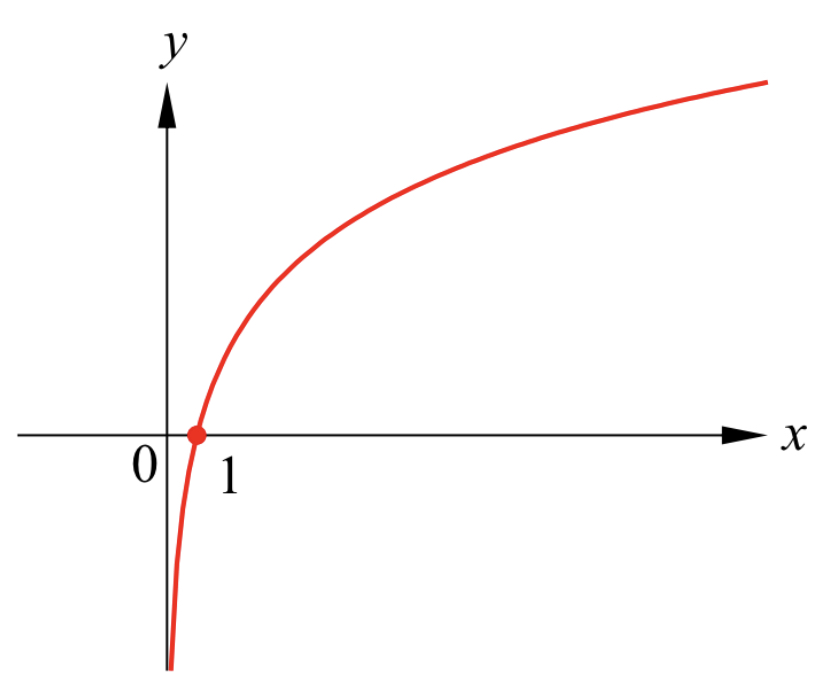
\includegraphics[scale=0.2]{Picture26.png}
\caption{  The function $y=\ln x$.\fa}\label{figure26}
\end{figure}
The following gives some useful properties of the natural logarithmic function.
\begin{proposition}[label=prop230217_5]{Properties of the Natural Logarithm Function}
Let $x$ and $y$ be any positive numbers, and let $r$ be a rational number. We have the following.
\begin{enumerate}[(a)]
\item $\ln (xy)=\ln x+\ln y$
\item $\ln\di \frac{x}{y}=\ln x-\ln y$
\item $\ln x^r=r\ln x$

\end{enumerate}
\end{proposition}
In part (c), we require $r$ to be a rational number since we have not defined $x^r$ when $r$ is an irrational number.
\begin{myproof}{Proof}
To prove (a), we fixed $y>0$ and define the function $f:(0,\infty)\to\mathbb{R}$ by
\[f(x)=\ln(xy)-\ln y.\] 
Then $f(1)=\ln y-\ln y=0$, and
\[f'(x)=\frac{y}{xy}=\frac{1}{x}.\]
By the uniquesness asserted in Theorem \ref{thm230217_3} and the definition of the natural logarithm function, we conclude that $f(x)=\ln x$. This proves (a).\bp

To prove (b), we notice that part (a) gives
\[ \ln\left(\frac{x}{y}\right)+\ln y=\ln\left(\frac{x}{y}\times y\right)=\ln x.\] 

For (c), notice that it is obvious if $r=0$. If $r\neq 0$,   define the function $f:(0,\infty)\to\mathbb{R}$ by
\[f(x)= \frac{1}{r}\ln x^r.\]   Then $f(1)=0$, and
\[f'(x)=\frac{1}{r}\times\frac{rx^{r-1}}{x^r}=\frac{1}{x}.\]
This allows us to conclude that $f(x)=\ln x$, and (c) is thus proved.



\end{myproof}

From part (b) of Proposition \ref{prop230217_5}, we find that for any $x>0$,
\[\ln \frac{1}{x}= \ln x^{-1}=-\ln x;\]
and if $n$ is a positive integer, 
\[\ln x^n=n\ln x.\]
In particular, we find that
\[\ln 2^n=n\ln 2,\]
\[\ln \frac{1}{2^n}=-n\ln 2.\]
Since $\ln 2>0$, we conclude the following.
\begin{proposition}{}
$f:(0, \infty)\to\mathbb{R}$, $f(x)=\ln x$ is a strictly increasing function with
\[\lim_{x\rightarrow 0^+}\ln x=-\infty,\hspace{1cm}\lim_{x\to \infty}\ln x=\infty.\]
Hence, the range of $f(x)=\ln x$ is $\mathbb{R}$. 
\end{proposition}

\subsection{The Exponential Functions}
Since the function $f:(0,\infty)\to\mathbb{R}$, $f(x)=\ln x$ is continuous and strictly increasing, its inverse function exists. We define this inverse function as the exponential function $\exp(x)$. The domain of $\exp(x)$ is the range of $\ln x$, which is $\mathbb{R}$. The range of $\exp(x)$ is the domain of $\ln x$, which is $(0, \infty)$.
\begin{definition}{The Natural Exponential Function}
The natural exponential function $\exp :\mathbb{R}\to \mathbb{R}$ is defined to be the inverse of the function $ \ln x$. It satisfies
\[\ln \exp(x)=x \quad\text{for any}\;x\in\mathbb{R},\hspace{1cm}
 \exp(\ln x)=x\quad\text{for any}\;x>0.\]
\end{definition}

\begin{figure}[ht]
\centering
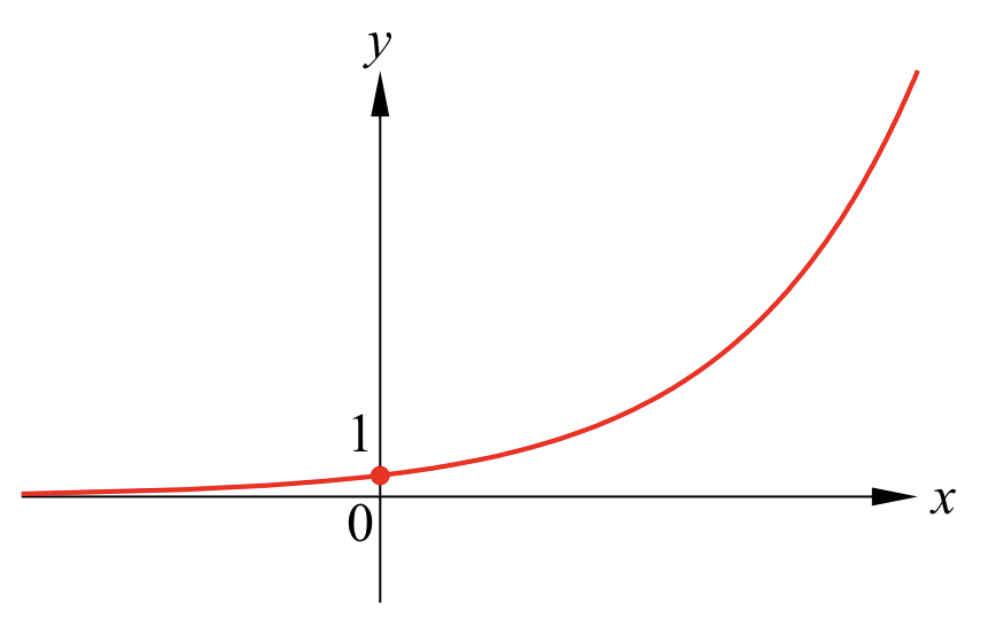
\includegraphics[scale=0.2]{Picture27.png}
\caption{  The function $y=\exp(x)$.\fa}\label{figure27}
\end{figure}
We can deduce the following properties.
\begin{proposition}{Properties of the Natural Exponential Function I}
The exponential function $\exp(x)$ is a strictly increasing differentiable function defined on the set of real numbers. It has the following properties.
\begin{enumerate}[(a)]
\item $\exp(x)>0$ for all $x\in\mathbb{R}$ and $\exp(0)=1$.
\item $\di\lim_{x\to-\infty}\exp(x)=0$, $\di\lim_{x\to \infty}\exp(x)=\infty$.
\item $\di\frac{d}{dx}\exp(x)=\exp(x)$.


\end{enumerate}
\end{proposition}
\begin{myproof}{Proof}
(a) and (b) are obvious from the corresponding properties of $\ln x$.
 For part (c), we employ the derivative formula for inverse function. To make it less confusing, let $y=\exp(x)$. Then
\[\ln y=x.\]
Differentiating both sides with respect to $x$, we find that
\[ \frac{1}{y}\frac{dy}{dx}=1.\]Therefore,
\[\frac{d}{dx}\exp(x)=\frac{dy}{dx}=y=\exp(x).\]

\end{myproof}

From the properties of the natural logarithm stated in Proposition \ref{prop230217_5}, we have the following.
\begin{proposition}{Properties of the Natural Exponential Function II}
Let $x$ and $y$ be any real numbers, and let $r$ be a rational number. We have the following.
\begin{enumerate}[(a)]
\item $\exp(x+y)=\exp(x)\exp(y)$.
\item $\exp(x-y)=\di \frac{\exp(x)}{\exp(y)}$.
\item $\exp(x)^r=\exp(rx)$.\end{enumerate}
\end{proposition}
\begin{myproof}{Proof}
Let $u=\exp(x)$ and $v=\exp(y)$. Then $u$ and $v$ are positive numbers and
\[x=\ln u,\hspace{1cm}y=\ln v.\]
By Proposition \ref{prop230217_5},
\[\ln(uv)=\ln u+\ln v=x+y.\]\bp
Therefore,
\[\exp(x)\exp(y)=uv=\exp(x+y).\]
Part (b) is proved in the same way. For part (c),
Proposition \ref{prop230217_5} implies that
\[\ln(u^r)=r\ln u=rx.\]
Therefore,
\[\exp(x)^r=u^r=\exp(rx).\]
\end{myproof}

Notice that part (c) says that for any postive number $u$, and any rational number $r$, 
\[u^r=\exp(r\ln u).\]We can use this to define power functions with    irrational powers.
\begin{definition}{Power Functions}
For any real number $r$, the power function $f(x)=x^r$ is the function defined on $(0, \infty)$ by the formula
\[x^r=\exp(r\ln x).\] When $r>0$, we can extend the definition to the point $x=0$ by definining $f(0)=0$.
\end{definition}


We have seen that this definition coincides with the old definition when $r$ is a rational number. 
For $r>0$, since $\ln x\to -\infty$ as $x\to 0^+$, $r\ln x\to -\infty$ as $x\to 0^+$. Since $\exp(x)\to 0$ as $x\to -\infty$, we conclude that $x^r\to 0$ as $x\to 0^+$. Therefore, the definition $f(0)=0$ makes the function $f(x)=x^r$ continuous.
Using the fact that $\exp(x)$ and $\ln x$ are inverses of each other, we have the following.
\begin{highlight}{}
For any positive number $x$ and any real number $r$,
\[\ln (x^r)=r\ln x.\]
\end{highlight}

\begin{figure}[ht]
\centering
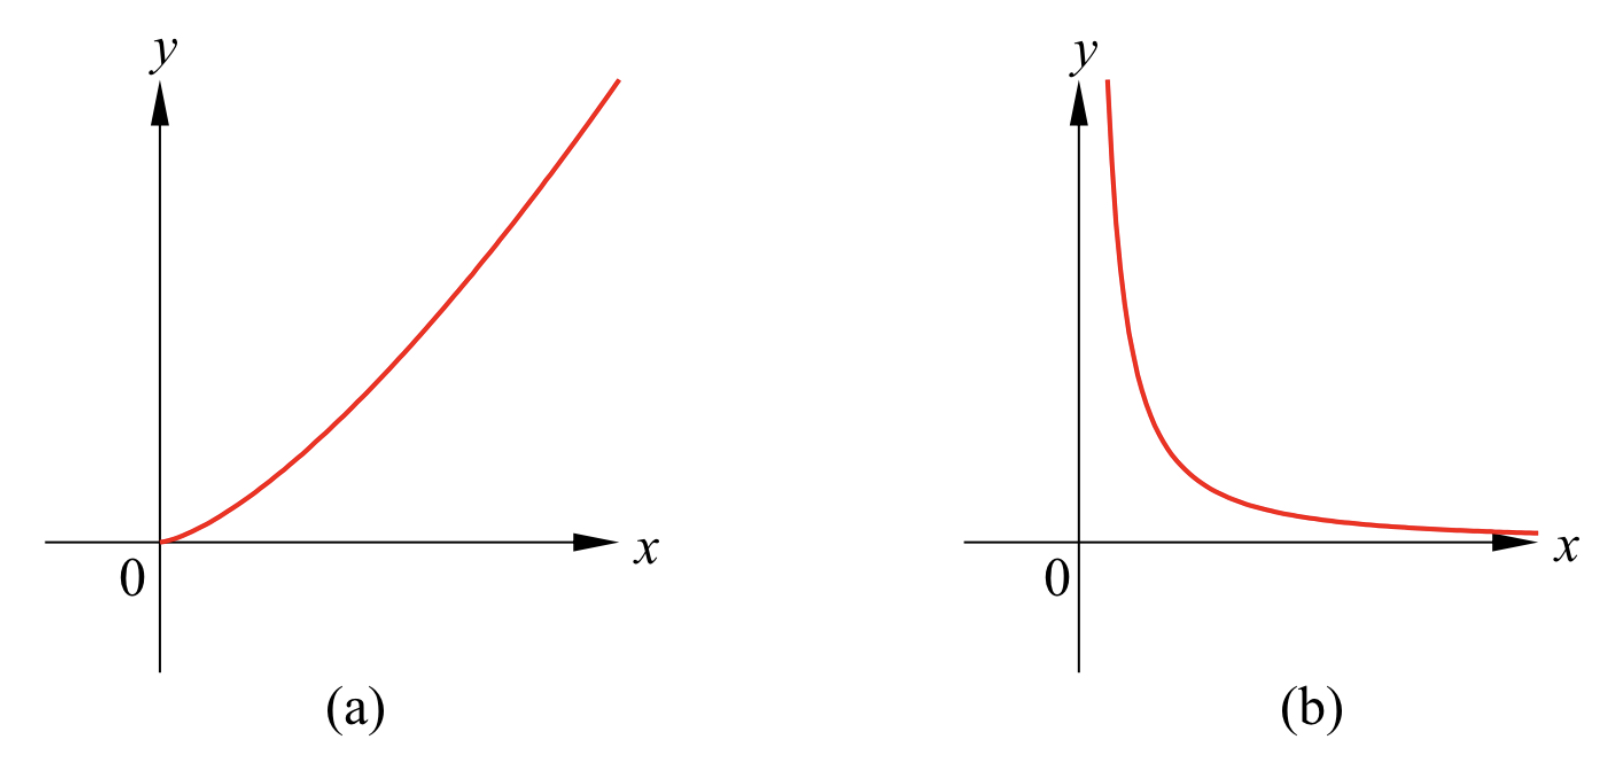
\includegraphics[scale=0.2]{Picture28.png}
\caption{ (a) The function $y=x^{\sqrt{2}}$.   (b) The function $y=x^{-\sqrt{2}}$.\fa}\label{figure28}
\end{figure}

Since both $\ln x$ and $\exp(x)$ are strictly increasing functions, it is easy to deduce the following.
\begin{highlight}{Monotonicity of Power Functions}
\begin{enumerate}[1.]
\item When $r>0$, the function $f:[0,\infty)\to\mathbb{R}$, $f(x)=x^r$ is strictly increasing.
\item When $r<0$, the function $f:(0,\infty)\to\mathbb{R}$, $f(x)=x^r$ is strictly decreasing.
\end{enumerate}
\end{highlight}

The following gives the properties of power functions.
\begin{proposition}{}
For any positive numbers $x$ and $y$, and any real numbers $r$ and $s$,
\begin{enumerate}[(a)]
\item $\di (xy)^r=x^ry^r$
\item $\di \left(\frac{x}{y}\right)^r=\frac{x^r}{y^r}$
\item $x^{r+s}=x^rx^s$
\item $\di x^{r-s}=\frac{x^r}{x^s}$
\item $(x^r)^s=x^{rs}$

\end{enumerate}
\end{proposition}
\begin{myproof}{Proof}For part (a), we have
\begin{align*}
(xy)^r&=\exp\left(r\ln(xy)\right)=\exp(r\ln x+r\ln y)\\&=\exp(r\ln x)\exp(r\ln y)=x^ry^r.
\end{align*}Part (b) is proved in the same way. For part (c),
\[x^{r+s}=\exp\left((r+s)\ln x\right)=\exp(r\ln x)\exp(s\ln x)=x^rx^s.\]
Part (d) is proved in the same way.  For part (e),
\[(x^r)^s=\exp\left(s\ln (x^r)\right)=\exp\left(rs\ln x\right)=x^{rs}.\]
\end{myproof}

Using chain rule, we find that $f(x)=x^r$ is a differentiable function.
\begin{proposition}{}
For any real number $r$ and any positive number $x$,
\[\frac{d}{dx}x^r=rx^{r-1}.\]
\end{proposition}
\begin{myproof}{Proof}
This follows from straightforward computation.
\[\frac{d}{dx}x^r=\frac{d}{dx}\exp\left(r\ln x\right)= \exp(r\ln x)\frac{d}{dx}(r\ln x)=x^r\times\frac{r}{x}=rx^{r-1}.\]
\end{myproof}

Now we want to show that $\exp(1)=e$, where $e$ is the number we defined as
\[e=\lim_{n\to \infty}\left(1+\frac{1}{n}\right)^n\] in Chapter \ref{ch1}.

\begin{theorem}[label=thm230218_1]{} We have
\[\exp(1) =\lim_{n\to\infty}\left(1+\frac{1}{n}\right)^n=e.\]This imples that
\[\ln e=1.\]
\end{theorem}
\begin{myproof}{Proof}
We consider the differentiable function $g(x)=\ln (1+x)$, $x>-1$, whose derivative is
\[g'(x)=\frac{1}{1+x}.\]   By definition of derivative, 
\[\lim_{x\to 0}\frac{\ln(1+x)}{x}=\lim_{x\to 0}\frac{g(x)-g(0)}{x-0}=g'(0)=1.\]
Since $\exp(x)$ is a continuous function, we find that
\begin{equation}\label{eq230217_7}\lim_{x\to 0 }\exp\left(\frac{\ln(1+x)}{x}\right)=\exp\left(\lim_{x\to 0 }\frac{\ln(1+x)}{x}\right)= \exp(1).\end{equation} 
Notice that $\{1/n\}$ is a sequence of positive numbers that converges to 0. Therefore, eq. \eqref{eq230217_7} implies that
\[\lim_{n\to \infty}\exp\left(n\ln\left(1+\frac{1}{n}\right)\right)=\exp(1).\] 
By definition,\[\exp\left(n\ln\left(1+\frac{1}{n}\right)\right)=\left(1+\frac{1}{n}\right)^n.\] Thus, we have shown that
\[\exp(1) =\lim_{n\to\infty}\left(1+\frac{1}{n}\right)^n=e.\]
Since $\exp(x)$ and $\ln x$ are inverses of each other, we find that $\ln e=1$.
\end{myproof}
 
\begin{definition}{General Exponential Functions}
Let $a$ be a positive real number such that $a\neq 1$. The exponential function $f(x)=a^x$ is defined by
\[a^x=\exp\left(x\ln a\right),\hspace{1cm}x\in\mathbb{R}.\]
When $a=e$, $f(x)=e^x$ is the natural exponential function 
\[e^x=\exp(x).\]
\end{definition}
Henceforth, we will also use $e^x$ to denote the natural exponential function $\exp(x)$. 


The following properties of the general exponential functions can be easily derived from the  corresponding properties of the $\exp(x)$ function.  
\begin{proposition}{}Let $a$ be a positive number.
\begin{enumerate}[1.]
\item When $0<a<1$, $f(x)=a^x$ is a strictly decreasing function.
\item When $a>1$, $f(x)=a^x$ is a strictly increasing function.

\end{enumerate}
\end{proposition}
\begin{proposition}{}
Let $a$ be a positive number such that $a\neq 1$. The function $f(x)=a^x$ is differentiable, and 
\[\frac{d}{dx}a^x=a^x\ln a.\]
\end{proposition}

\begin{proposition}{}Let $a$ be a positive number such that $a\neq 1$. For any real numbers $x$ and $y$, 
\begin{enumerate}[1.]
\item  $a^{x+y}=a^xa^y$
\item $a^{x-y}=\di\frac{a^x}{a^y}$
\item $(a^x)^y=a^{xy}$
\end{enumerate}
\end{proposition}

\subsection{The Trigonometric Functions}
Now we consider the trigonometric functions.  
Recall that an angle is usually measured in degrees, so that the angle of a full circle is $360^{\circ}$. But for analysis, we need to make a change of units to radians.

\begin{figure}[ht]
\centering
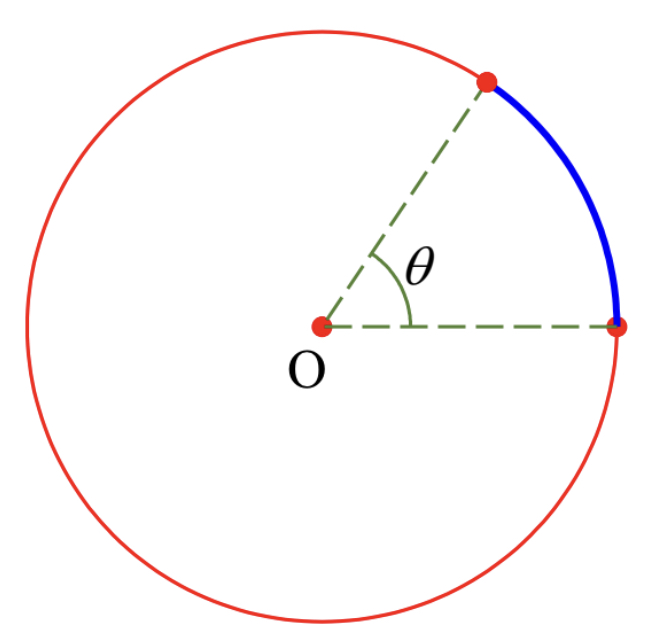
\includegraphics[scale=0.2]{Picture29.png}
\caption{An arc with central angle $\theta$.\fa}\label{figure29}
\end{figure}
The number $\pi$ is defined as the ratio of the circumsference of a circle to its diameter. Hence, a circle of radius 1 would have circumsference $2\pi$. This  number $\pi$ can be shown to be an irrational number. The radian measurement of an angle is so   that an arc with central angle $\theta$ radians on a circle of radius $r$ has length $r\theta$, so that the circumsference of the circle is $2\pi r$. Hence, the conversion between degrees and radians is
\[\theta^{\circ} =\frac{\pi}{180}\theta \,\text{rad}.\]



Historically, sine and cosine are defined using right-angled triangles, as shown in Figure \ref{figure30}.
\begin{figure}[ht]
\centering
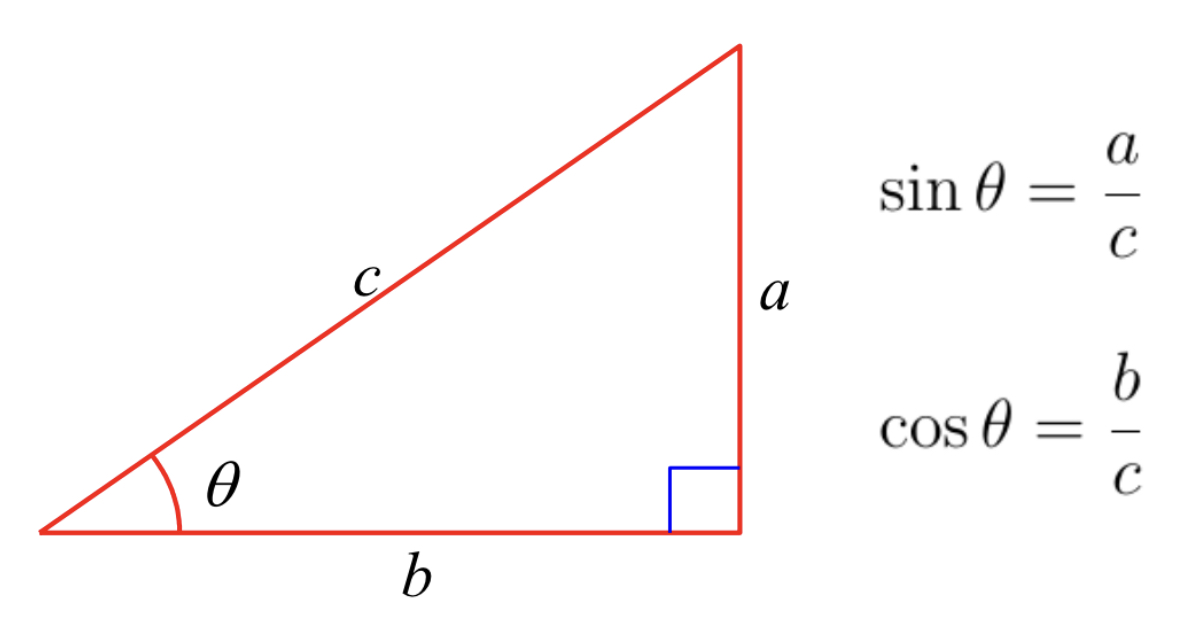
\includegraphics[scale=0.2]{Picture30.png}
\caption{Classical definitions of sine and cosine functions.\fa}\label{figure30}
\end{figure}

To extend the definitions of $\sin\theta$ and $\cos\theta$ so that $\theta$ can be any real numbers, we use the unit circle $x^2+y^2=1$. 
The angle measurement starts from the positive $x$-axis and we take the counter-clockwie direction as positive direction. 
For any real number $\theta$, 
find a point $P(x, y)$ on the unit circle such that the line segment between the origin $O$ and the point $P$ makes an angle $\theta$ radians with the positive $x$-axis (see Figure \ref{figure31}). Then we define $\cos\theta$ and $\sin\theta$ to be the $x$ and $y$ coordinates of $P$:
\[x=\cos\theta, \hspace{1cm} y=\sin\theta.\]

\begin{figure}[ht]
\centering
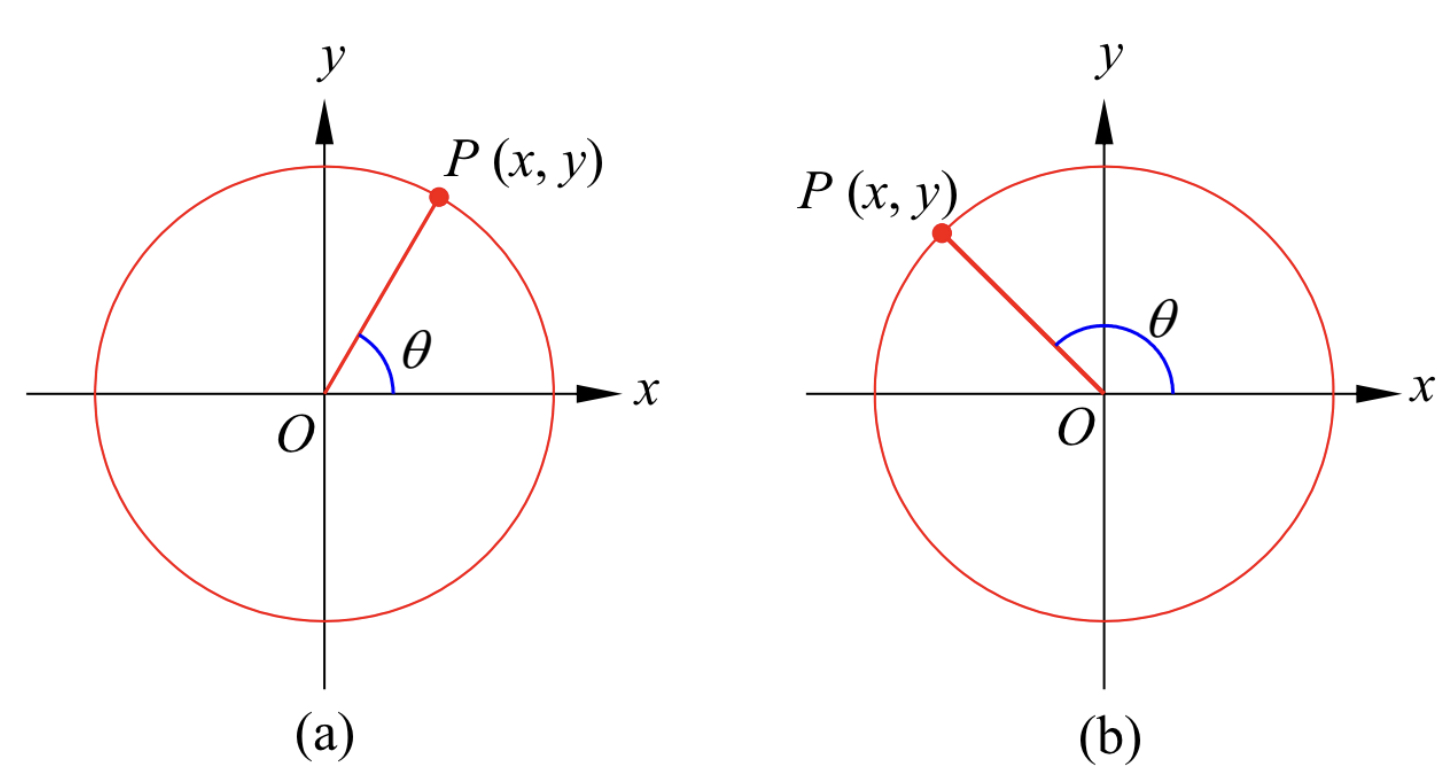
\includegraphics[scale=0.2]{Picture31.png}
\caption{The definitions of $\sin\theta$ and $\cos\theta$ for   (a)  $\di \theta=\frac{7\pi}{3}$ and  (b)  $\di\theta =\frac{3\pi}{4}$.\fa}\label{figure31}
\end{figure}
In this way, the function $\sin\theta$ and $\cos\theta$ are defined rigorously, and when $\theta$ is an acute angle, it coincides with the definition using right-angled triangles. From the definitions, it is obvious that $\sin\theta$ and $\cos\theta$ are periodic functions of periodic $2\pi$.

\begin{definition}{Periodic Functions}
A   function $f:\mathbb{R}\to\mathbb{R}$ is said to be periodic if there is a positive number $L$ so that
\[f(x+L)=f(x)\hspace{1cm}\text{for all}\; x\in \mathbb{R}.\]
Such a number $L$ is called a period of the function $f$. If $L$ is a period of $f$, then for any positive integer $n$, $nL$ is also a period of $f$.
\end{definition}

From the definitions, it is quite obvious that $\sin\theta$ and $\cos\theta$ are continuous functions. A rigorous proof is tedious. To show that these two functions are differentiable is also possible, but complicated. Two crucial formulas are
\begin{subequations}\label{eq230218_6}
\begin{align}
\sin(\theta_1+\theta_2)&=\sin\theta_1\cos\theta_2+\cos\theta_1\sin\theta_2,\label{eq230218_6a}\\
\cos(\theta_1+\theta_2)&=\cos\theta_1\cos\theta_2-\sin\theta_1\sin\theta_2.\label{eq230218_6b}
\end{align}\end{subequations}The proofs of these two formulas by elementary means are tedious.

In this section, we are going to define the sine and cosine functions using a different approach. We will show that the functions thus defined agree with the old definitions.

First, we present an existence and uniquess theorem.
\begin{theorem}[label=thm230218_3]{Existence and Uniqueness Theorem}
Let $\alpha$ and $\beta$ be any two real numbers. There exists a unique twice  differentiable function $f:\mathbb{R}\to\mathbb{R}$ satisfying
\[f''(x)+f(x)=0,\hspace{1cm}f(0)=\alpha,\;f'(0)=\beta.\]
\end{theorem}
Again, the proof of the existence requires knowledge from later chapters. We will prove uniqueness here. We begin by a lemma that will be useful later.
\begin{lemma}[label=lemma230218_5]{}Let  
 $f:\mathbb{R}\to\mathbb{R}$ be a twice differentiable  function that satisfies
\[f''(x)+f(x)=0.\]The following holds.
\begin{enumerate}[1.]
\item
  $f$ is infinitely differentiable. 
\item For any positive integer $n$, the $n^{\text{th}}$ derivative of $f$, $g(x)=f^{(n)}(x)$,   satisfies 
\[g''(x)+g(x)=0.\]
\item The function 
$ f(x)^2+f'(x)^2$ is  a constant.\end{enumerate}
\end{lemma}
\begin{myproof}{Proof}
Since $f$ is twice differentiable, $f$ is  continuous and differentiable. Since
$f''(x)=-f(x)$,   $f''$ is   continuous and differentiable.  This implies that $f$ is three times differentiable and $f'''=-f'$. Continue arguing in this way, we find that $f$ is infinitely differentiable, and for any nonengative integer $n$, \[f^{(n+2)}{x}=-f^{(n)}(x).\] The latter says that if $g=f^{(n)}$, then
\[g''(x)+g(x)=0.\]
These prove the first and second statements. For the third statement, 
we notice that
\begin{align*}\frac{d}{dx}\left(f'(x)^2+f(x)^2\right)&=f'(x)f''(x)+f(x)f'(x)\\&=2f'(x)\left(f''(x)+f(x)\right)=0.\end{align*}
This implies that $f(x)^2+f'(x)^2$ is  a constant.
\end{myproof}
Now we return to Theorem  \ref{thm230218_3}.
\begin{myproof}{\linkt   Proof of Theorem \ref{thm230218_3}}
If $f_1$ and $f_2$ are two functions that satisfy the given conditions, then the function $f=(f_1-f_2):\mathbb{R}\to\mathbb{R}$ is a  twice   differentiable function
satifying
\[f''(x)+f(x)=0,\hspace{1cm}f(0)=0,\; f'(0)=0.\]
To prove uniqueness, we only need to show that this function $f$ must be identically zero. 
By Lemma \ref{lemma230218_5}, there is a constant $C$ such that 
\[f'(x)^2+f(x)^2=C.\]
Setting $x=0$, we find that $C=0$. Hence,
\[f'(x)^2+f(x)^2=0.\]\bp
Since the square of a nonzero number is always positive, we must have
\[f(x)=f'(x)=0\hspace{1cm}\text{for all}\;x\in \mathbb{R}.\]
This completes the proof that $f$ is identically zero.

\end{myproof}
Notice that for a function $f:\mathbb{R}\to\mathbb{R}$ that satisfies $f''(x)+f(x)=0$, we have
\[f^{(4)}(x)=-f''(x)=f(x).\]
This implies that for all positive integers $n$,
\[f^{(4n)}(x)=f(x),\quad f^{(4n+1)}(x)=f'(x),\]
\[f^{(4n+2)}(x)=f''(x),\quad f^{(4n+3)}(x)=f'''(x).\]If $f$ is the unique solution to \[f''(x)+f(x)=0,\hspace{1cm}f(0)=\alpha,\; f'(0)=\beta,\] then its derivative $g=f'$ is the unique solution to
\[g''(x)+g(x)=0,\hspace{1cm}g(0)=\beta,\; g'(0)=-\alpha.\]

\begin{definition}{The Sine and Cosine functions}
The sine function $S(x)=\sin x$ is defined to be   the unique twice   differentiable function satisfying
\[S''(x)+S(x)=0,\hspace{1cm}S(0)=0,\;S'(0)=1.\]The cosine function $C(x)=\cos x$ is defined as the derivative of $S(x)$. Namely, 
$C(x)=S'(x)$. It is the unique twice differentiable function satisfying
\[C''(x)+C(x)=0, \hspace{1cm}C(0)=1,\;C'(0)=0.\]
\end{definition}


Notice that once we prove the existence of the function $S(x)=\sin x$, then the function $C(x)=\cos x$ exists. One can then check that the function
\[f(x)=\alpha C(x)+\beta S(x)\] is a twice differentiable function satifying \[f''(x)+f(x)=0,\hspace{1cm}f(0)=\alpha,\;f'(0)=\beta.\]In other words, to prove the existence part in Theorem 
\ref{thm230218_3}, we only need to establish the existence of the function $S(x)=\sin x$.


In the following, we establish the properties of the functions $S(x) $ and $C(x) $.

\begin{theorem}[label=thm230218_7]{}
The functions $S(x)$ and $C(x)$ are infinitely differentiable functions that satisfy  the following.
\begin{enumerate}[(a)]
\item $S'(x)=C(x)$ and $C'(x)=-S(x)$ for all $x\in\mathbb{R}$.
\item $S(x)$ is an odd function, $C(x)$ is an even function.
\item $S(x)^2+C(x)^2=1$ for all $x\in\mathbb{R}$.
\item For any real numbers $x$ and $y$, $S(x+y)=S(x)C(y)+C(x)S(y)$.
\item  For any real numbers $x$ and $y$, $C(x+y)=C(x)C(y)-S(x)S(y)$.

\end{enumerate}
\end{theorem}
\begin{myproof}{Proof} 
$S'(x)=C(x)$ is  by the definition of $C(x)$. Differentiating gives $C'(x)=S''(x)=-S(x)$. To prove (b), one check that the function $f(x)=-S(-x)$ satisfies
$f''(x)+f(x)=0$, $f(0)=0$ and $f'(0)=1$. By uniquess of the function $S(x)$, we have $f(x)=S(x)$, which proves that $S(x)$ is an odd function. Since $C(x)=S'(x)$, $C(x)$ is an even function.
Lemma \ref{lemma230218_5} says that $S(x)^2+S'(x)^2$ is a constant. Hence, there is a constant $A$ such that
\[S(x)^2+C(x)^2=A\hspace{1cm}\text{for all}\;x\in\mathbb{R}.\]
Setting $x=0$ gives $A=1$. This proves part (c). For part (d), fixed a real number $y$ and consider the function
\[f(x)=S(x+y).\]\bp
We find that \[f'(x)=S'(x+y)=C(x+y),\]  
\[f''(x)+f(x)=S''(x+y)+S(x+y)=0,\]
and
\[f(0)=S(y),\hspace{1cm}f'(0)=C(y).\]
Since the function $g(x)=S(y)C(x)+C(y)S(x)$  satisfies
\[g''(x)+g(x)=0,\hspace{1cm}g(0)=S(y),\;g'(0)=C(y),\]
by uniquesness, we find that $f(x)=g(x)$ for all $x\in \mathbb{R}$. Therefore,
\[S(x+y)=S(x)C(y)+C(x)S(y).\]
Differentiate with respect to $x$ gives
\[C(x+y)=C(x)C(y)-S(x)S(y).\]
\end{myproof}

Here we have used advanced analytic tools to prove the identities \eqref{eq230218_6} in a simple way.  Part (c) in Theorem \ref{thm230218_7} says that
\[\sin^2 x+\cos^2 x=1\hspace{1cm}\text{for all}\;x\in\mathbb{R}.\]
This implies that
\[|\sin x|\leq 1,\hspace{1cm} |\cos x|\leq 1\hspace{1cm}\text{for all}\;x\in\mathbb{R}.\]By definition, $\sin 0=S(0)=0$ and $\cos 0=C(0)=1$. What is not obvious is that  0 is in the range of $C(x)$. 
\begin{theorem}[label=thm230218_8]
{}
There is a smallest positive number $u$ such that $C(u)=0$. 
\end{theorem}
\begin{myproof}{Proof}
Since $S(x)$ is differentiable, we can apply mean value theorem to conclude that there is a point $v$ in $(0, 2)$ such that
\[\frac{S(2)-S(0)}{2-0}=S'(v)=C(v).\]
This gives
\[|C(v)|=\frac{1}{2}|S(2)|\leq\frac{1}{2}.\]By part (e) and part (c) in Theorem \ref{thm230218_7},
\[C(2v)= C(v)^2-S(v)^2= 2C(v)^2-1\leq \frac{1}{2}-1<0.\]
Since $C(2v)<0<C(0)$, and $C(x)$ is a continuous function, intermediate value theorem implies that there is a point $w$ in $(0, 2v)$ such that $C(w)=0$. Let 
\[A=\left\{w>0\,|\, C(w)=0.\right\}.\] We have just shown that $A$ is a nonempty set. By definition, $A$ is bounded below by 0. Hence, $u=\inf A$ exists. By Lemma \ref{23020510}, there is a sequence $\{w_n\}$ in $A$ that converges to $u$. Since $C(x)$ is continuous, the sequence $\{C(w_n)\}$ converges to $C(u)$. But $C(w_n)=0$ for all $n$. Hence, $C(u)=0$. Since $C(0)=1$, $u\neq 0$. Hence, $u>0$. This proves that 
$u$ is the smallest positive number such that $C(u)=0$. \end{myproof}

Let $u$ be the smallest positive number such that $C(u)=0$. Then we must have $C(x)>0$ for all $x\in [0, u)$. Since $S'(x)=C(x)$, $S(x)$ is strictly increasing on $[0, u]$. Thus, $S(x)>0$ for all $x\in (0, u]$. This, and $S(u)^2+C(u)^2=1$, implies that $S(u)=1$.
From part (d) and part (e) in Theorem \ref{thm230218_7}, we find that
\begin{subequations}
\begin{align*}
S(x+u)&=S(x)C(u)+C(x)S(u)=C(x),\\
C(x+u)&=C(x)C(u)-S(x)S(u)=-S(x).
\end{align*}
\end{subequations}It follows that
\begin{subequations}
\begin{align*}
S(x+2u)&=C(x+u)=-S(x),\\
C(x+2u)&= -S(x+u)=-C(x).
\\
S(x+3u)&=C(x+2u)=-C(x),\\
C(x+3u)&= -S(x+2u)=S(x).
\\
S(x+4u)&=C(x+3u)=S(x),\\
C(x+4u)&= -S(x+3u)=C(x).
\end{align*}
\end{subequations}The last pair of equations show that $S(x)$ and $C(x)$ are periodic functions of period $4u$. Since $S(x)>0$ and $C(x)>0$ for $x\in (0,u)$, we have the following.
\begin{enumerate}[$\bullet$\;\;]
\item For $x\in (0, u)$, $C(x)>0$, $S(x)>0$.
\item For $x\in (u, 2u)$, $C(x)<0$, $S(x)>0$.
\item For $x\in (2u, 3u)$, $C(x)<0$, $S(x)<0$.
\item For $x\in (3u, 4u)$, $C(x)>0$, $S(x)<0$.
\end{enumerate}
Together with $S(0)=0$, $C(0)=1$,  $S(u)=1$, $C(u)=0$, we find that $S(2u)=0$, $C(2u)=-1$, $S(3u)=-1$, $C(3u)=0$. These imply that for every $P(x, y)$ on the unit circle $x^2+y^2=1$, there is a unique $\theta\in [0, 4u)$ such that
\[x=C(\theta), \quad y=S(\theta).\]
 What is not obvious is that this $\theta$ is exactly the radian of the angle that the line segment $OP$ makes with the positive $x$-axis. To show this, we can argue in the following way. Assume that an object is travelling on the circle $x^2+y^2=1$, and its position at time $t$ is $(x(t), y(t))$, where
\[x=C(t), \quad y=S(t).\]
It follows that the velocity of the object at time $t$ is $(x'(t), y'(t))$, where
\[x'(t)=-S(t),\quad y'(t)=C(t).\]
This implies that the speed is
\[\sqrt{x'(t)^2+y'(t)^2}=\sqrt{S(t)^2+C(t)^2}=1.\]
Hence, the object is travelling at a constant speed 1. The distance travelled up to time $t$ is then $t$. This proves that the arclength of the arc from $(1,0)$ to the point $P(C(t), S(t))$ is $t$. Then $t$ must be the radian of the angle $OP$ makes with the positive $x$ axis. Hence, the functions $C(t)$ and $S(t)$ coincide with the classical $\cos t$ and $\sin t$ functions. Having proved this, by the definition of $\pi$, we have
\[2u=\pi.\]
Hence, we can summarize the facts above as follows.
\begin{highlight}{Properties of the Sine and Cosine Functions}
The functions $S(x)=\sin x$ and $C(x)=\cos x$ are $2\pi$ periodic infinitely differentiable functions. 
\[\frac{d}{dx}\sin x=\cos x,\hspace{1cm}\frac{d}{dx}\cos x=-\sin x.\]

Moreover, they have the following properties.
\begin{enumerate}[1.]
\item $\sin\left(x+\frac{\pi}{2}\right)=\cos x$, $\cos\left(x+\frac{\pi}{2}\right)=-\sin x$.
\item $\sin\left(x+\pi\right)=-\sin x$, $\cos\left(x+\pi \right)=-\cos x$.
\item $\sin\left(x+\frac{3\pi}{2}\right)=-\cos x$, $\cos\left(x+\frac{3\pi}{2}\right)=\sin x$.
\item $\sin x$ is an odd function, $\cos x$ is an even function.
\item $\sin x=0$ if and  only if $x=n\pi$, where $n$ is an integer.
\item $\cos x=0$ if and only if $x=\left(n+\frac{1}{2}\right)\pi$,  where $n$ is an integer.
\end{enumerate}
\end{highlight}


\begin{figure}[ht]
\centering
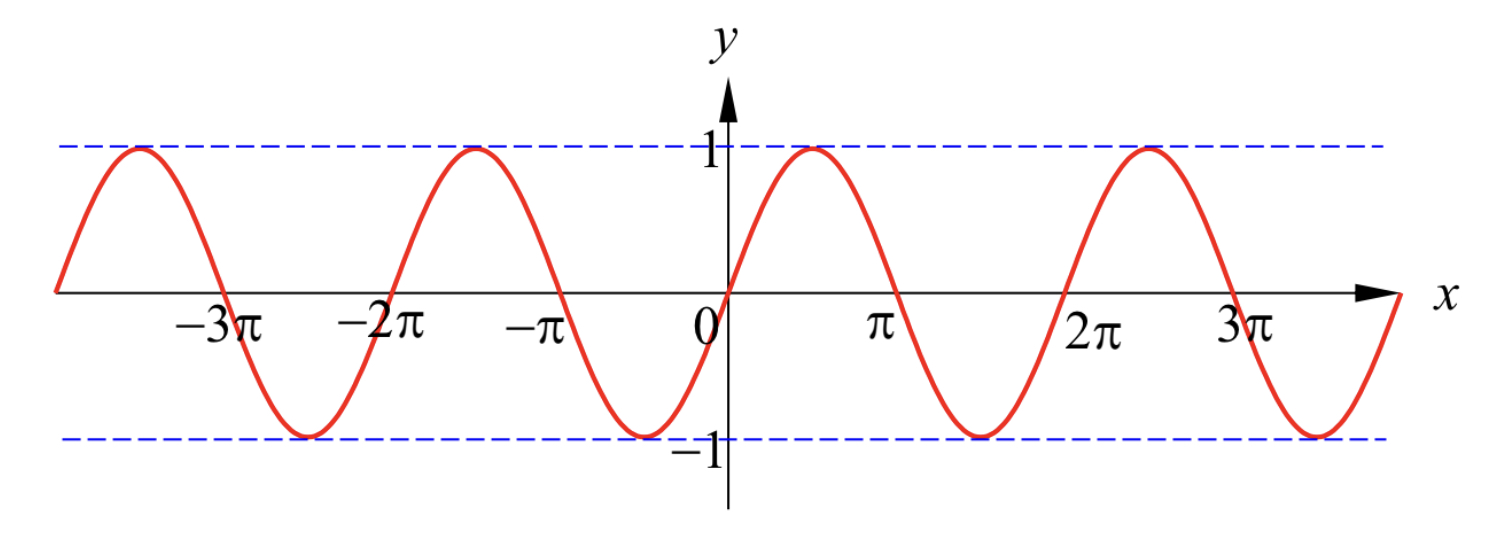
\includegraphics[scale=0.2]{Picture32.png}
\caption{The sine function $S(x)=\sin x$.\fa}\label{figure32}
\end{figure}



\begin{figure}[ht]
\centering
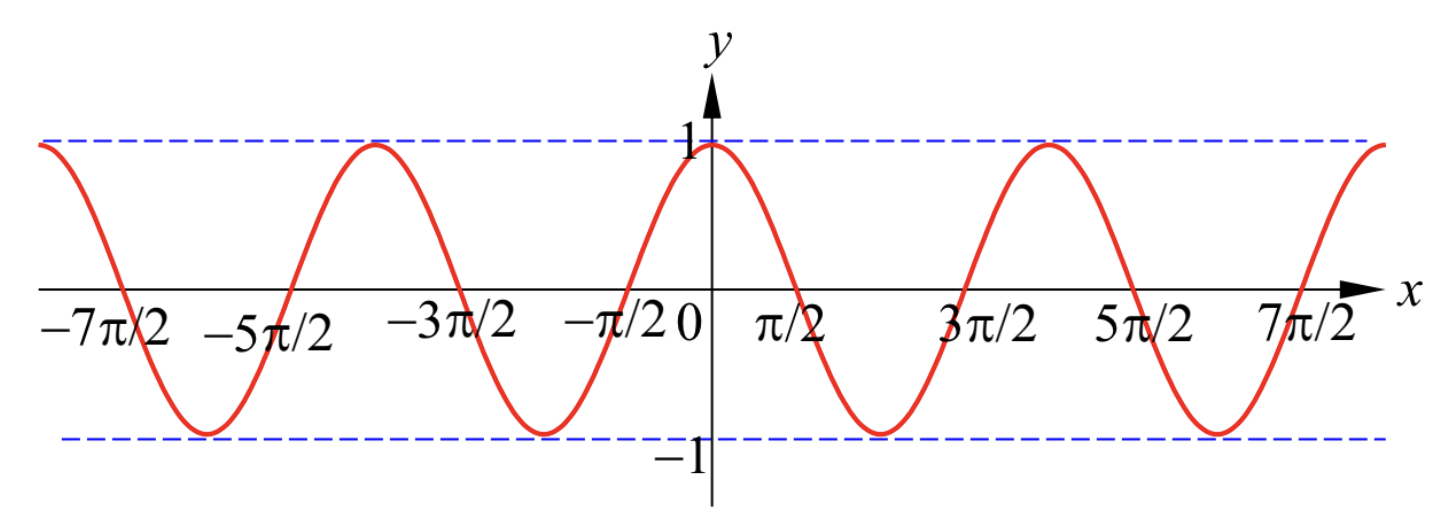
\includegraphics[scale=0.2]{Picture33.png}
\caption{The cosine function $C(x)=\cos x$.\fa}\label{figure33}
\end{figure}

There are four other trigonometric functions. They are defined in terms of $\sin x$ and $\cos x$ in the usual way.
\begin{definition}{Trigonmetric Functions}
The tangent, cotangent, secant and cosecant functions are defined as
\begin{align*}
\tan x&=\frac{\sin x}{\cos x},\hspace{1cm}\sec x=\frac{1}{\cos x},\hspace{1cm} x\neq \left(n+\frac{1}{2}\right)\pi, n\in\mathbb{Z};\\
\cot x&=\frac{\cos x}{\sin x},\hspace{1cm}\csc x=\frac{1}{\sin x},\hspace{1cm} x\neq n\pi, n\in\mathbb{Z}.\end{align*}
\end{definition}


\begin{figure}[ht]
\centering
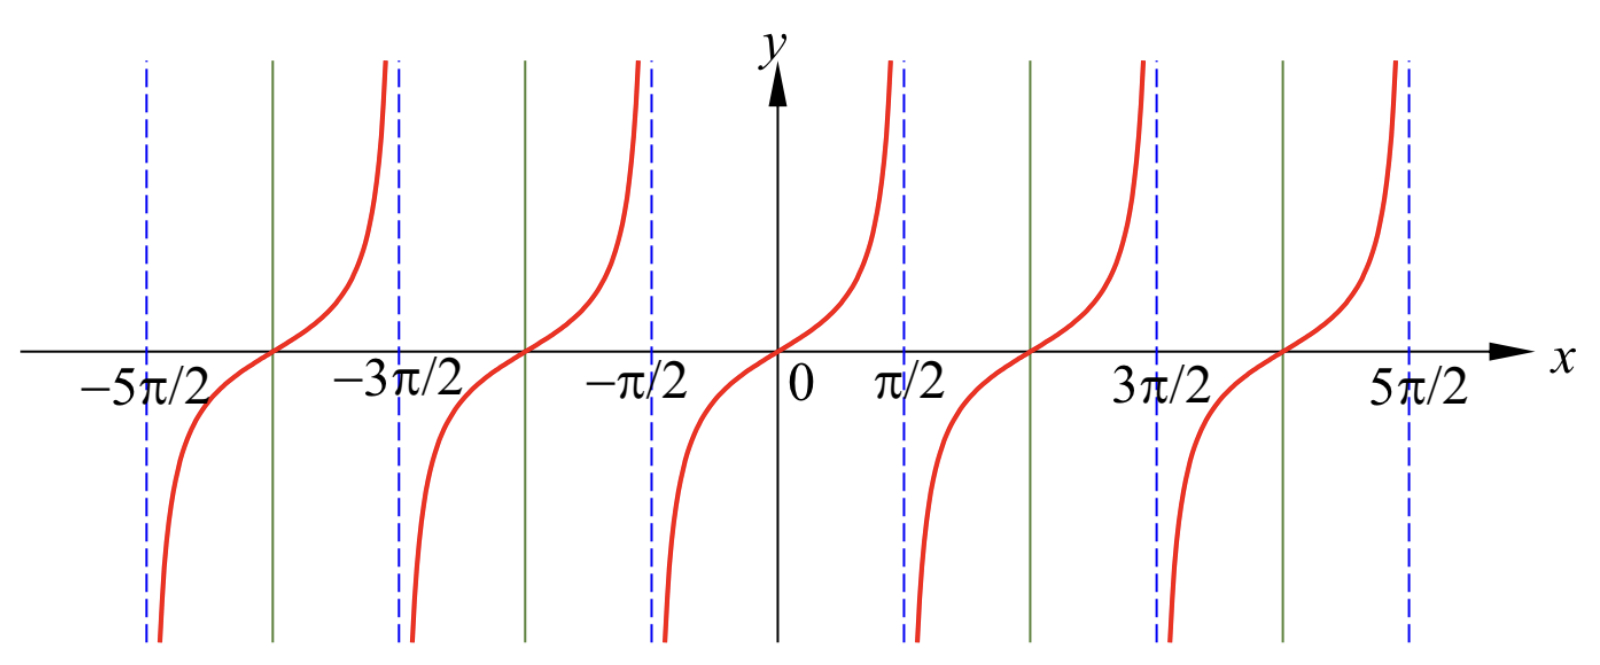
\includegraphics[scale=0.2]{Picture34.png}
\caption{The   function $f(x)=\tan x$.\fa}\label{figure34}
\end{figure}
The  following are easy to derive.
\begin{proposition}{}
$\tan x$, $\cot x$, $\sec x$ and $\csc x$ are infinitely differentiable functions with
\begin{align*}
\frac{d}{dx}\tan x&=\sec^2 x,\hspace{1.8cm} \frac{d}{dx}\cot x=-\csc^2x,\\
\frac{d}{dx}\sec x&=\sec x\tan x,\hspace{1cm}\frac{d}{dx}\csc x=-\csc x\cot x.
\end{align*}
\end{proposition}

Before closing this subsection, we want to prove some important limits and  inequalities for the function $\sin x$.
\begin{theorem}[label=230307_8]{}
\begin{enumerate}[1.]
\item
For any real number $x$, $|\sin x|\leq |x|$.
\item $\di \lim_{x\to 0}\frac{\sin x}{x}=1$.
\item For any $x\in [0, \pi/2]$, 
\[\frac{2}{\pi}x\leq \sin x \leq x.\]
\end{enumerate}
\end{theorem}
\begin{myproof}{Proof}
 
When $x=0$, $\sin x=0$ and $|\sin x|\leq |x|$ is obviously true. If $x\neq 0$, mean value theorem implies that there is a number $c$ in $(0,1)$ such that
\begin{equation}\label{eq230218_9}\frac{\sin x}{x}=\frac{\sin x-\sin 0}{x-0}=\cos (cx).\end{equation}
Hence, \[\left|\frac{\sin x}{x}\right|=|\cos (cx)|\leq 1,\]which implies that $|\sin x|\leq |x|$. This proves the first statement.\bp
For the second statement, the definition of derivative implies that
\begin{equation*}\lim_{x\to 0}\frac{\sin x}{x}=\lim_{x\to 0}\frac{\sin x-\sin 0}{x-0}=\left.\frac{d}{dx}\right|_{x=0}\sin x=\cos 0=1.\end{equation*}
  For the third statement, define the function $g:[0,\frac{\pi}{2}]\to\mathbb{R}$ by
\[g(x)=\begin{cases}\di\frac{\sin x}{x},\quad &\text{if}\;0<x\leq\di\frac{\pi}{2},\\1,\quad &\text{if}\;x=0.\end{cases}\]Then $g$ is continuous on $[0, \frac{\pi}{2}]$, and differentiable on $(0, \frac{\pi}{2})$, with
\[g'(x)=\frac{x\cos x-\sin x}{x^2}=\frac{1}{x}\left(\cos x-\frac{\sin x}{x}\right)\hspace{1cm}\text{when}\;0<x<\frac{\pi}{2}.\]
As before, for each $x\in (0, \frac{\pi}{2}]$, mean value theorem implies that there is a $u\in (0, x)$ such that
\[\frac{\sin x}{x}=\cos u.\]
Since $0<u<x$ and the cosine function is strictly decreasing on $(0, \frac{\pi}{2})$, we find that
\[g'(x)=\frac{1}{x}\left(\cos x-\frac{\sin x}{x}\right)=\frac{1}{x}\left(\cos x-\cos u\right)<0.\]
This shows that $g:[0,\frac{\pi}{2}]\to\mathbb{R}$ is a strictly decreasing function. Since $g(0)=1$ and $g(\frac{\pi}{2})=\frac{2}{\pi}$, we find that for all $x\in (0, \frac{\pi}{2}]$,
\[\frac{2}{\pi}\leq\frac{\sin x}{x}\leq 1.\]
Thus, for all $x\in [0, \pi/2]$, 
\[\frac{2}{\pi}x\leq \sin x \leq x.\]

\end{myproof}



\subsection{The Inverse Trigonometric Functions}
In this section, we are going to define inverse functions for $\sin x$, $\cos x$ and $\tan x$.
Since trigonometric functions are periodic functions, they are not one-to-one. Hence, we cannot find their inverses over the whole domain of their definitions. However, we can restrict each of  their domains to  an interval on which each of  them is one-to-one to define the inverse. Such interval should contain the interval $(0, \pi/2)$ which is where these functions are classically defined. 

\begin{enumerate}[$\bullet$\;\;]
\item The largest interval that contains  the interval $(0, \pi/2)$ and on which $\sin x$ is one-to-one is $[-\frac{\pi}{2}, \frac{\pi}{2}]$.
\item The largest interval that contains  the interval $(0, \pi/2)$ and on which $\cos x$ is one-to-one is $[0, \pi]$.
\item The largest interval that contains  the interval $(0, \pi/2)$ and on which $\tan x$ is one-to-one is $(-\frac{\pi}{2}, \frac{\pi}{2})$.
\end{enumerate}

\begin{definition}{Inverse Sine Function }
  The function  $\sin^{-1}x$ is a function defined on $[-1, 1]$ and with range $[-\frac{\pi}{2}, \frac{\pi}{2}]$ such that
\begin{align*}\sin(\sin^{-1}x)&=x\hspace{1cm}\text{for all}\;x\in[-1,1];\\
\sin^{-1}(\sin x)&=x\hspace{1cm}\text{for all}\; x\in\left[-\frac{\pi}{2}, \frac{\pi}{2}\right].\end{align*}
 

\end{definition}
\begin{definition}{Inverse Cosine Function }
  The function  $\cos^{-1}x$ is a function defined on $[-1, 1]$ and with range $[0, \pi]$ such that
\begin{align*}\cos(\cos^{-1}x)&=x\hspace{1cm}\text{for all}\;x\in[-1,1];\\
\cos^{-1}(\cos x)&=x\hspace{1cm}\text{for all}\; x\in [0, \pi].\end{align*}
 

\end{definition}
\begin{definition}{Inverse Tangent Function }
  The function  $\tan^{-1}x$ is a function defined on $\mathbb{R}$ and with range $(-\frac{\pi}{2}, \frac{\pi}{2})$ such that
\begin{align*}\tan(\tan^{-1}x)&=x\hspace{1cm}\text{for all}\;x\in\mathbb{R};\\
\tan^{-1}(\tan x)&=x\hspace{1cm}\text{for all}\; x\in \left(-\frac{\pi}{2}, \frac{\pi}{2}\right).\end{align*}
 

\end{definition}
The differentiability of the inverse trigonometric functions and their derivative formulas follow  immediately from Theorem \ref{thm230218_9}.

\begin{theorem}{}
$\sin^{-1}:(-1,1)\to \mathbb{R}$ is a differentiable function with
\[\frac{d}{dx}\sin^{-1}x=\frac{1}{\sqrt{1-x^2}}.\]
\end{theorem}

\begin{theorem}{}
$\cos^{-1}:(-1,1)\to \mathbb{R}$ is a differentiable function with
\[\frac{d}{dx}\cos^{-1}x=-\frac{1}{\sqrt{1-x^2}}.\]
\end{theorem}

\begin{theorem}{}
$\tan^{-1}:\mathbb{R}\to \mathbb{R}$ is a differentiable function with
\[\frac{d}{dx}\tan^{-1}x=\frac{1}{1+x^2}.\]
\end{theorem}
\vp


\noindent
{\bf \large Exercises  \thesection}
\setcounter{myquestion}{1}
\begin{question}{\themyquestion}
Determine the following limits.
\begin{enumerate}[(a)]
\item
$\di\lim_{n\to \infty}\left(1-\frac{1}{n}\right)^n$
\item
$\di\lim_{n\to \infty}\left(1+\frac{2}{n}\right)^n$
\item
$\di\lim_{n\to \infty}\left(1-\frac{2}{n}\right)^n$
 
\end{enumerate}
\end{question}
\atc
 
 
\begin{question}{\themyquestion}
For any $x\in [-1,1]$, show that $\sin^{-1}x+\cos^{-1}x$ is a constant and find this constant.
\end{question}
\atc
\begin{question}{\themyquestion}
Determine the following limits.
\begin{enumerate}[(a)]
\item
$\di\lim_{x\to \frac{\pi}{2}^-}\tan x$
\item
$\di\lim_{x\to -\frac{\pi}{2}^+}\tan x$
\item
$\di\lim_{x\to -\infty}\tan^{-1} x$
\item
$\di\lim_{x\to \infty}\tan^{-1} x$
\end{enumerate}
\end{question}

\atc
 
 
\begin{question}{\themyquestion}
Consider the function $f:\mathbb{R}\to\mathbb{R}$ defined by
\[f(x)=\begin{cases} \di \sin\left(\frac{1}{x}\right),\quad &\text{if}\;x\neq 0,\\
0,\quad &\text{if}\;x= 0.\end{cases}\]
Determine whether $f$ is a continuous function. If not, find the points where the function $f$ is not continuous.
\end{question}

\atc
 
 
\begin{question}{\themyquestion}
Consider the function $f:\mathbb{R}\to\mathbb{R}$ defined by
\[f(x)=\begin{cases} \di x\sin\left(\frac{1}{x}\right),\quad &\text{if}\;x\neq 0,\\
0,\quad &\text{if}\;x= 0.\end{cases}\]
Show that $f$ is a continuous function.
\end{question}

\atc
 
 
\begin{question}{\themyquestion}
Consider the function $f:\mathbb{R}\to\mathbb{R}$ defined by
\[f(x)=\begin{cases} \di x^2\sin\left(\frac{1}{x}\right),\quad &\text{if}\;x\neq 0,\\
0,\quad &\text{if}\;x= 0.\end{cases}\]Let $g:\mathbb{R}\to\mathbb{R}$ be the function defined by
\[g(x)=x+f(x).\]
\begin{enumerate}[(a)]
\item Show that $f$ is a differentiable function.
\item Show that $f':\mathbb{R}\to\mathbb{R}$ is not continuous.
\item Show that $g'(0)=1$, but for any neighbourhood $(a,b)$ of 0,   $g:(a,b)\to\mathbb{R}$ is not increasing.
\end{enumerate}
\end{question}

 
\vp
\section{L' H$\hat{\text{o}}$pital's Rules}\label{sec3.6}
In this section, we will apply the Cauchy mean value theorem to prove the l' H$\hat{\text{o}}$pital's rules. The latter are useful rules for finding limits of the form
\[\lim_{x\to x_0}\frac{f(x)}{g(x)},\]
when we have one of the following two indeterminate forms.
\begin{enumerate}[1.]
\item Type $0/0$, where
$\di\lim_{x\to x_0}f(x)=0$ and $\di\lim_{x\to x_0}g(x)=0$.
\item Type $\infty/\infty$, where $\di\lim_{x\to x_0}f(x)=\infty$ and $\di\lim_{x\to x_0}g(x)=\infty$.
\end{enumerate}
Here $x_0$ can be $\infty$ or $-\infty$.

Let us first prove the following special case.
\begin{theorem}[label=thm230216_14]{}
Let $f:(a,b)\to\mathbb{R}$ and $g:(a,b)\to\mathbb{R}$ be differentiable functions that satisfy the following conditions.
\begin{enumerate}[(i)]
\item $\di\lim_{x\rightarrow a^+}f(x)=\lim_{x\rightarrow a^+}g(x)=0$.
\item $\di\lim_{x\rightarrow a^+}\frac{f'(x)}{g'(x)}=L$.

\end{enumerate}
Then $\di \lim_{x\rightarrow a^+}\frac{f(x)}{g(x)}=L$.
\end{theorem}
\begin{myproof}{Proof}
The condition (i) implies that we can extend $f$ and $g$ to be continuous functions on $[a, b)$ by defining $f(a)=g(a)=0$. Then by Cauchy mean value theorem, for any $x\in (a, b)$, there is a point $u(x)\in (a, x)$ such that
\begin{equation}\label{eq230216_15}\frac{f(x)}{g(x)}=\frac{f(x)-f(a)}{g(x)-g(a)}=\frac{f'(u(x))}{g'(u(x))}.\end{equation}\bp
 Since 
\[a<u(x)<x,\]
squeeze theorem implies that
\[\lim_{x\to a^+}u(x)=a.\] 
By limit law for composite functions, we find that
\[\lim_{x\to a^+}\frac{f'(u(x))}{g'(u(x))}=\lim_{u\to a^+}\frac{f'(u)}{g'(u)}=L.\]
By \eqref{eq230216_15}, this proves that
\[\lim_{x\rightarrow a^+}\frac{f(x)}{g(x)}=L.\]
\end{myproof}

It is easy to see that an analogue of Theorem \ref{thm230216_14} holds for left limits.  Combine the left limit and the right limit, we have the following.

\begin{theorem}[label=thm230216_16]{l' H$\hat{\text{o}}$pital's Rule I}
Let $x_0$ be a point in the open interval $(a, b)$, and let   $D=(a,b)\setminus\{x_0\}$. Given that $f:D\to\mathbb{R}$ and $g:D\to\mathbb{R}$ are diferentiable  functions that satisfy the following conditions.
\begin{enumerate}[(i)]
\item $\di\lim_{x\rightarrow x_0}f(x)=\lim_{x\rightarrow x_0}g(x)=0$.
\item  $\di\lim_{x\rightarrow x_0}\frac{f'(x)}{g'(x)}=L$.

\end{enumerate}
Then  we have $\di \lim_{x\rightarrow x_0}\frac{f(x)}{g(x)}=L$.
\end{theorem}
 We return to a problem that we discussed earlier.
\begin{example}{}Determine the limit \[\lim_{x\to 1}\frac{x^{20}+2x^9-3}{x^7-1}\] if it exists.
\end{example}
\begin{solution}{Solution}
Let $f(x)=x^{20}+2x^9-3$ and $g(x)=x^7-1$. Then
\[\lim_{x\to 1}f(x)=f(1)=0\hspace{1cm} \text{and}\hspace{1cm} \lim_{x\to 1}g(x)=g(1)=0.\]
$f$ and $g$ are continuously differentiable functions with
\[f'(x)=20x^{19}+18x^8\hspace{1cm} \text{and}\hspace{1cm}  g'(x)=7x^6.\]
Since\[\lim_{x\to 1}\frac{f'(x)}{g'(x)}=\lim_{x\to 1}\frac{20x^{19}+18x^8}{7x^6}=\frac{38}{7},\]
l' H$\hat{\text{o}}$pital's rule implies that
\[\lim_{x\to 1}\frac{x^{20}+2x^9-3}{x^7-1}=\frac{38}{7}.\]
\end{solution}
Let us look at some other examples.
\begin{example}{}
Determine whether the limit exists. If it exists, find the limit.
\begin{enumerate}[(a)]
\item
$\di \lim_{x\to 0}\frac{e^x-1-x}{x^2}$
\item $\di \lim_{x\to 0}\frac{\sin 2x}{3x}$
\item $\di \lim_{x\to 0}\frac{\cos 2x-1}{x^2}$
\end{enumerate}
\end{example}
\begin{solution}{Solution}
\begin{enumerate}[(a)]
\item
This is a limit of the form $0/0$. Applying l' H$\hat{\text{o}}$pital's rule, we have
\[\lim_{x\to 0}\frac{e^x-1-x}{x^2}=\lim_{x\to 0}\frac{e^x-1}{2x}.\]
Again, we have a limit of the form $0/0$. Applying l' H$\hat{\text{o}}$pital's rule again, we have
\[\lim_{x\to 0}\frac{e^x-1-x}{x^2}=\lim_{x\to 0}\frac{e^x-1}{2x}=\lim_{x\to 0}\frac{e^x}{2}=\frac{1}{2}.\]
\item This is a limit of the form $0/0$.  Apply l' H$\hat{\text{o}}$pital's rule, we have
\[\lim_{x\to 0}\frac{\sin 2x}{3x}=\lim_{x\to 0}\frac{2\cos 2x}{3}=\frac{2}{3}.\]
\item This is a limit of the form $0/0$. Applying l' H$\hat{\text{o}}$pital's rule twice, we have
\[\lim_{x\to 0}\frac{\cos 2x-1}{x^2}=\lim_{x\to 0}\frac{-2\sin 2x}{2x}=\lim_{x\to 0}\frac{-4\cos 2x}{2}=-2.\]
\end{enumerate}
\end{solution}
 
Using l' H$\hat{\text{o}}$pital's rule, we can give a second solution to Example \ref{ex230216_17}.
\begin{example}{}
 Since $f$ is continuous, we have
\[\lim_{h\to 0}\left(f(x_0+h)+f(x_0-h)-2f(x_0)\right)=0.\]Since we also have $\di\lim_{h\to 0}h^2=0$, we can apply l' H$\hat{\text{o}}$pital's rule to get
\[\lim_{h\to 0}\frac{f(x_0+h)+f(x_0-h)-2f(x_0)}{h^2} =\lim_{h\to 0}\frac{f'(x_0+h)-f'(x_0-h) }{2h}.\] 
 Since $f'$ is  continuous, \[\lim_{h\to 0}\left(f'(x_0+h)-f'(x_0-h) \right)=0.\]\be Since we also have $\di\lim_{h\to 0}(2h)=0$, applying l' H$\hat{\text{o}}$pital's rule again give
\[\lim_{h\to 0}\frac{f'(x_0+h)-f'(x_0-h) }{2h}=\lim_{h\to 0}\frac{f''(x_0+h)+f''(x_0-h)}{2}.\]
It follows from the continuity of $f''$ that
\[ \lim_{h\to 0}\frac{f''(x_0+h)+f''(x_0-h)}{2}=f''(x_0).\]These prove that
\[\lim_{h\to 0}\frac{f(x_0+h)+f(x_0-h)-2f(x_0)}{h^2}  =f''(x_0).\]

\end{example2}

 

In the future, we are going to see that Taylor's approximation is an alternative to l' H$\hat{\text{o}}$pital's rule when the point $x_0$ is finite and the indeterminate form if of the type $0/0$. However, when $x_0$ is infinite or the indeterminate form is of type $\infty/\infty$,  l' H$\hat{\text{o}}$pital's rule becomes useful.

The following is for the case where $x_0$ is infinite, and the limit is of the form $0/0$.
\begin{theorem}[label=thm230216_18]{l' H$\hat{\text{o}}$pital's Rule II}
Let $a$ be a positive number. Given that $f:(a,\infty)\to\mathbb{R}$ and $g:(a,\infty)\to\mathbb{R}$ are diferentiable  functions that satisfy the following conditions.
\begin{enumerate}[(i)]
\item $\di\lim_{x\rightarrow \infty}f(x)=\lim_{x\rightarrow \infty}g(x)=0$.
\item  $\di\lim_{x\rightarrow \infty}\frac{f'(x)}{g'(x)}=L$.

\end{enumerate}
Then  we have $\di \lim_{x\rightarrow \infty}\frac{f(x)}{g(x)}=L$.
\end{theorem}
\begin{myproof}{Proof}
Let $b=1/a$, and define the functions $f_1:(0, b)\to\mathbb{R}$ and $g_1:(0,b)\to\mathbb{R}$ by
\[f_1(x)=f\left(\frac{1}{x}\right),\hspace{1cm}g_1(x)=g\left(\frac{1}{x}\right).\]  Then $f_1$ and $g_1$ are differentiable functions and
\[f_1'(x)=-\frac{1}{x^2}f'\left(\frac{1}{x}\right),\hspace{1cm}g_1'(x)=-\frac{1}{x^2}g'\left(\frac{1}{x}\right).\]
Moreover,
\[\lim_{x\to 0^+}f_1(x)=\lim_{x\to\infty}f(x)=0,\hspace{1cm}\lim_{x\to 0^+}g_1(x)=\lim_{x\to\infty}g(x)=0,\]
and
\[\lim_{x\to 0^+}\frac{f_1'(x)}{g_1'(x)}=\lim_{x\to 0^+}\frac{f'\left(\frac{1}{x}\right)}{g'\left(\frac{1}{x}\right)}=\lim_{x\to\infty}\frac{f'(x)}{g'(x)}=L.\]
By Theorem \ref{thm230216_14}, 
\[\lim_{x\to 0^+}\frac{f_1(x)}{g_1 (x)}=L.\]This implies that 
\[ \lim_{x\rightarrow \infty}\frac{f(x)}{g(x)}=L.\]
\end{myproof}

 Let us look at the following example.
\begin{example}{}
Determine whether the limit $\di\lim_{x\to \infty}\left(\frac{x}{x+2}\right)^{x+1}$ exists. If it exists, find the limit.
\end{example}
This is not of the type $0/0$. But the logarithm of it can be turned into that form.
\begin{solution}{Solution}
Consider the function 
\[g(x)=\ln \left(\frac{x}{x+2}\right)^{x+1}=(x+1)\ln \left(\frac{x}{x+2}\right).\]
When $x\to \infty$, we have something of the form $\infty \,\cdot\,0$. We turn it to the form $0/0$ by
\[g(x)=\frac{\di \ln\left(\frac{x}{x+2}\right)}{\di \frac{1}{x+1}}=\frac{\ln x-\ln(x+2)}{\di \frac{1}{x+1}}.\]
 l' H$\hat{\text{o}}$pital's rule implies that
\begin{align*}\lim_{x\to\infty}g(x)&=\lim_{x\to\infty}\frac{\di\frac{1}{x}-\frac{1}{x+2}}{-\di \frac{1}{(x+1)^2}}\\
&=-2\lim_{x\to \infty}\frac{x^2+2x+1}{x^2+2x}\\
&=-2.
\end{align*}
By continuity of the exponential function, we have
\[\lim_{x\to \infty}\left(\frac{x}{x+2}\right)^{x+1}=\lim_{x\to \infty}e^{g(x)}=\exp\left(\lim_{x\to \infty}g(x)\right)=e^{-2}.\]
\end{solution}


Suppose we want to find the limit
\begin{equation}\label{eq230218_2}\lim_{x\rightarrow \infty}\frac{x}{e^x}.\end{equation}
This is a limit of the form $\infty/\infty$. One may say that we can turn it to a limit of the form $0/0$ by writing
\[\frac{x}{e^x}=\frac{e^{-x}}{x^{-1}}.\]
Then l' H$\hat{\text{o}}$pital's rule says that if the limit
\begin{equation}\label{eq230218_3}\lim_{x\to\infty}\frac{e^{-x}}{- x^{-2}}\end{equation} exists and is equal to $L$, the limit \eqref{eq230218_2} also exists and is equal to $L$. However, the limit \eqref{eq230218_3} is   more complicated than the limit \eqref{eq230218_2}. So this strategy is useless.
Hence, there is a need for us to consider the $\infty/\infty$ indeterminate case. We only  prove the theorem in the case $x_0$ is finite. The case where $x_0$ is infinite can be dealt with in the same way as in the proof of Theorem \ref{thm230216_18}.
 

\begin{theorem}[label=thm230216_19]{l' H$\hat{\text{o}}$pital's Rule III}
Let $x_0$ be a point in the open interval $(a, b)$, and let  $D$ be the set $D=(a,b)\setminus\{x_0\}$. Given that $f:D\to\mathbb{R}$ and $g:D\to\mathbb{R}$ are diferentiable  functions that satisfy the following conditions.
\begin{enumerate}[(i)]
\item $\di\lim_{x\rightarrow x_0}f(x)=\lim_{x\rightarrow x_0}g(x)=\infty$.
\item  $\di\lim_{x\rightarrow x_0}\frac{f'(x)}{g'(x)}=L$.

\end{enumerate}
Then  we have $\di \lim_{x\rightarrow x_0}\frac{f(x)}{g(x)}=L$.
\end{theorem}
 The proof of this theorem is technical because of the infinite limits. The strategegy to rewrite this as 
\[\lim_{x\to x_0}\frac{1/g(x)}{1/f(x)}\] is not useful, as have been demonstrated in our discussion before this theorem.
\begin{myproof}{Proof}
We will prove that  the right limit $\di \lim_{x\rightarrow x_0^+}\frac{f(x)}{g(x)}$ is equal to $L$. The proof that the left limit is equal to $L$ is similar.  
Observe that if we fix a point $u$ in $(x_0, b)$, then for any $x$ in $(x_0, u)$, Cauchy mean value theorem asserts that there is a $c_x$ in $(x, u)$ such that 
\[\frac{f(x)-f(u)}{g(x)-g(u)}=\frac{f'(c_x)}{g'(c_x)}.\]\bp
This implies that
\[\frac{(f(x)-Lg(x))-(f(u)-Lg(u))}{g(x)-g(u)}=\frac{f'(c_x)}{g'(c_x)}-L.\]Thus,
\begin{equation}\label{eq230217_2}\frac{f(x)}{g(x)}-L=\frac{g(x)-g(u)}{g(x)}\left(\frac{f'(c_x)}{g'(c_x)}-L\right)+\frac{f(u)-Lg(u)}{g(x)}.\end{equation}


Fixed $\varepsilon>0$. By assumption of
\[\lim_{x\rightarrow x_0^+}\frac{f'(x)}{g'(x)}=L,\]
  there exsits a $\delta_1>0$ such that $(x_0, x_0+\delta_1)\subset (a,b)$, and for any $x\in (x_0, x_0+\delta_1)$, 
\[\left|\frac{f'(x)}{g'(x)}-L\right|<\frac{\varepsilon}{3}.\]Take $u=x_0+\delta_1/2$. 
Since $\di \lim_{x\rightarrow x_0}g(x)=\infty$, we find that
\[\lim_{x\to x_0^+}\frac{g(x)-g(u)}{g(x)}=1\hspace{1cm}\lim_{x\to x_0^+}\frac{f(u)-Lg(u)}{g(x)}=0.\]
Therefore, there exists a number $\delta$ such that $0<\delta\leq\delta_1/2$, and for all $x\in (x_0, x_0+\delta)$,
\[\left|\frac{g(x)-g(u)}{g(x)}\right|<2,\hspace{1cm}\left|\frac{f(u)-Lg(u)}{g(x)}\right|<\frac{\varepsilon}{3}.\]
If $x$ is in $(x_0, x_0+\delta)$, $x_0<x<u$ and hence $x_0<c_x<u<x_0+\delta_1$. This implies that
\[\left|\frac{f'(c_x)}{g'(c_x)}-L\right|<\frac{\varepsilon}{3}.\] 
Eq. \eqref{eq230217_2} then implies that for all $x\in (x_0, x_0+\delta)$,
\begin{align*}
\left|\frac{f(x)}{g(x)}-L\right|&\leq \left|\frac{g(x)-g(u)}{g(x)}\right|\left| \frac{f'(c_x)}{g'(c_x)}-L\right|+\left|\frac{f(u)-Lg(u)}{g(x)}\right|\\
&<2\times\frac{\varepsilon}{3}+\frac{\varepsilon}{3}=\varepsilon.
\end{align*}\bp
This proves that 
\[ \lim_{x\rightarrow x_0^+}\frac{f(x)}{g(x)}=L.\]

 
\end{myproof} Notice that in the proof, we do not use the assumption that $\di\lim_{x\to x_0}f(x)=\infty$. Hence, this can be ommited from the conditions in the theorem. If $f(x)$ is bounded in a neighbourhood of $x_0$, there is no need to apply l' H$\hat{\text{o}}$pital's rule.

Let us now look at some examples.
\begin{example}[label=230307_11]{}
Let $r$ be a positive number.
Prove that
\[\lim_{x\to \infty}\frac{\ln x}{x^{r}}=0.\]
Deduce that for any positive number $s$,
\[\lim_{x\to \infty}x^se^{-x}=0.\]
\end{example}
\begin{solution}{Solution}
The limit \[\lim_{x\to \infty}\frac{\ln x}{x^{r}}\] is of the form $\infty/\infty$. Apply l' H$\hat{\text{o}}$pital's rule, we have
\[\lim_{x\to \infty}\frac{\ln x}{x^{r}}=\lim_{x\to\infty}\frac{\di \frac{1}{x}}{\di rx^{r-1}}=\frac{1}{r}\lim_{x\to \infty}\frac{1}{x^r}=0.\]  Since $\di\lim_{x\to \infty}e^x=\infty$, and the function $f(x)=x^s$ is a continuous function, we find that
\begin{align*}
\lim_{x\to\infty}x^se^{-x}&=\lim_{u\to \infty} \frac{(\ln u)^s}{u}\\
&=\left(\lim_{u\to \infty} \frac{\ln u}{u^{1/s}}\right)^s\\
&=0^s=0.
\end{align*}
\end{solution}
\begin{highlight}{}
The result of this example shows that when $x$ becomes large,\begin{enumerate}[$\bullet$\;\;]
\item $\ln x$ goes to infinity slower than any positive powers of $x$;
\item any positive powers of $x$ goes to infinity slower than $e^x$.\end{enumerate}
\end{highlight}

\begin{example}{}
Show that there exists a number $c$  so that the function
\[f(x)=\begin{cases} x^x,\quad &\text{if}\;x>0,\\
c,\quad &\text{if}\;x=0,\end{cases}\] is continuous.
\end{example}\begin{solution}{Solution}
Since
\[f(x)=x^x=e^{x\ln x}\hspace{1cm}\text{when}\;x>0,\] $f(x)$ is continuous on $(0, \infty)$.  To make $f$ continuous, $f$ must be continuous at $x=0$. This means
\[c=f(0)=\lim_{x\to 0^+}f(x)=\lim_{x\to 0^+}e^{x\ln x}.\]
Let us look at the limit $\di\lim_{x\to 0^+}x\ln x$. It is of the form $0\,\cdot\,\infty$. We turn it to the form $\infty/\infty$, and use l' H$\hat{\text{o}}$pital's rule.  
\[\lim_{x\to 0^+}x\ln x=\lim_{x\to 0^+}\frac{\ln x}{\di\frac{1}{x}}=\lim_{x\to 0^+}\frac{\di \frac{1}{x}}{-\di\frac{1}{x^2}}=-\lim_{x\to 0^+}x=0.\]Therefore, when
\[c=\exp\left(\lim_{x\to 0^+}x\ln x\right)=e^0=1,\]the function $f:[0, \infty)\to\mathbb{R}$ is continuous.
\end{solution}

\vp
\noindent
{\bf \large Exercises  \thesection}
\setcounter{myquestion}{1}

\begin{question}{\themyquestion}
Determine whether the limit exists. If it exists, find the limit.
\begin{enumerate}[(a)]
\item
$\di\lim_{x\to 1}\frac{x^{100}+x^{50}-2}{3x^{101}+4x^{55}-7x}$
\item $\di \lim_{x\to 0}\frac{2e^{-x}-2+2x}{x^2+3x^3}$
\item $\di\lim_{x\to 0}\frac{\tan^{-1}x}{x}$
\item $\di\lim_{x\to 0}\frac{\tan x-x}{x^3}$
\end{enumerate}
\end{question}
\atc
\begin{question}{\themyquestion}
Find the limit
\[\lim_{x\to \infty}\left(\frac{3x-1}{3x+1}\right)^{2x+1}.\]
\end{question}
\atc
\begin{question}{\themyquestion}
Let $r$ be a positive number. Prove that
\[\lim_{x\to 0^+}x^r\ln x=0.\]
\end{question}

 
\atc
\begin{question}{\themyquestion}
Determine whether the limit
 exists. If it exists, find the limit.
\begin{enumerate}[(a)]
\item
$\di \lim_{x\to 1}\frac{x^x-1}{x-1}$
\item $\di \lim_{x\to 0^+}\frac{x^x-1}{x\ln x}$
\item $\di \lim_{x\to 0^+}\frac{x^x\ln (1+x)}{x}$
\end{enumerate}
\end{question}


\vp

\section{Concavity of Functions}\label{sec3.7}

In this section, we study concavity of functions. If a function is twice differentiable, its concavity is determined by the second derivative.

Recall that if $x_1$ and $x_2$ are two points in $\mathbb{R}$, then as $t$ runs through all numbers in the interval $[0,1]$, 
\[x_1+t(x_2-x_1)=(1-t)x_1+tx_2\]runs through all points in the interval $[x_1, x_2]$. We say that a subset $S$ of $\mathbb{R}$ is convex if and only if for any two points $x_1$ and $x_2$ in $S$, and for any $t$ in $[0, 1]$, the point $(1-t)x_1+tx_2$ is also in $S$. We have proved that a subset of $\mathbb{R}$ is convex if and only if it is an interval.
\begin{definition}{Concavity of Functions}
Let $I$ be an interval.
\begin{enumerate}[1.]
\item A function $f:I\rightarrow \mathbb{R}$ is   concave up (or convex) provided that for any two points $x_1$ and $x_2$ in $I$, and for any $t\in [0,1]$,
    \[f((1-t)x_1+tx_2)\leq (1-t)f(x_1)+tf(x_2).\]
 \item A function $f:I\rightarrow \mathbb{R}$ is   concave down provided that for any  two points $x_1$ and $x_2$ in $I$, and for any $t\in [0,1]$,
   \[f((1-t)x_1+tx_2)\geq (1-t)f(x_1)+tf(x_2).\]
\item A function $f:I\rightarrow \mathbb{R}$ is strictly  concave up (or strictly convex)  provided that for any two distinct points $x_1$ and $x_2$ in $I$, and for any $t\in (0,1)$,
    \[f((1-t)x_1+tx_2)<(1-t)f(x_1)+tf(x_2).\]
 \item A function $f:I\rightarrow \mathbb{R}$ is strictly concave  down  provided that for any two distinct points $x_1$ and $x_2$ in $I$, and for any $t\in (0,1)$,
   \[f((1-t)x_1+tx_2)> (1-t)f(x_1)+tf(x_2).\]
\end{enumerate}
\end{definition}

Notice that a function $f:I\to\mathbb{R}$ is concave up if and only if the function $-f:I\to\mathbb{R}$ is concave down. Same for the strict concavity.

Geometrically, we draw a line   $L$ passing through the points $P_1(x_1, f(x_1))$  and $P_2(x_2, f(x_2))$ on the graph $y=f(x)$. If the equation of this line $L$ is $y=g(x)$, and $x_0=(1-t)x_1+tx_2$,  then 
\[g(x_0)= (1-t)f(x_1)+tf(x_2).\] Hence, $(x_0, g(x_0))$ is  point on the line $L$. Therefore, a function $y=f(x)$ is strictly concave up if its graph is always below a line segment joining two points on the graph; and it is strictly concave down if its graph is always above a line segment joining two points on the graph.


\begin{figure}[ht]
\centering
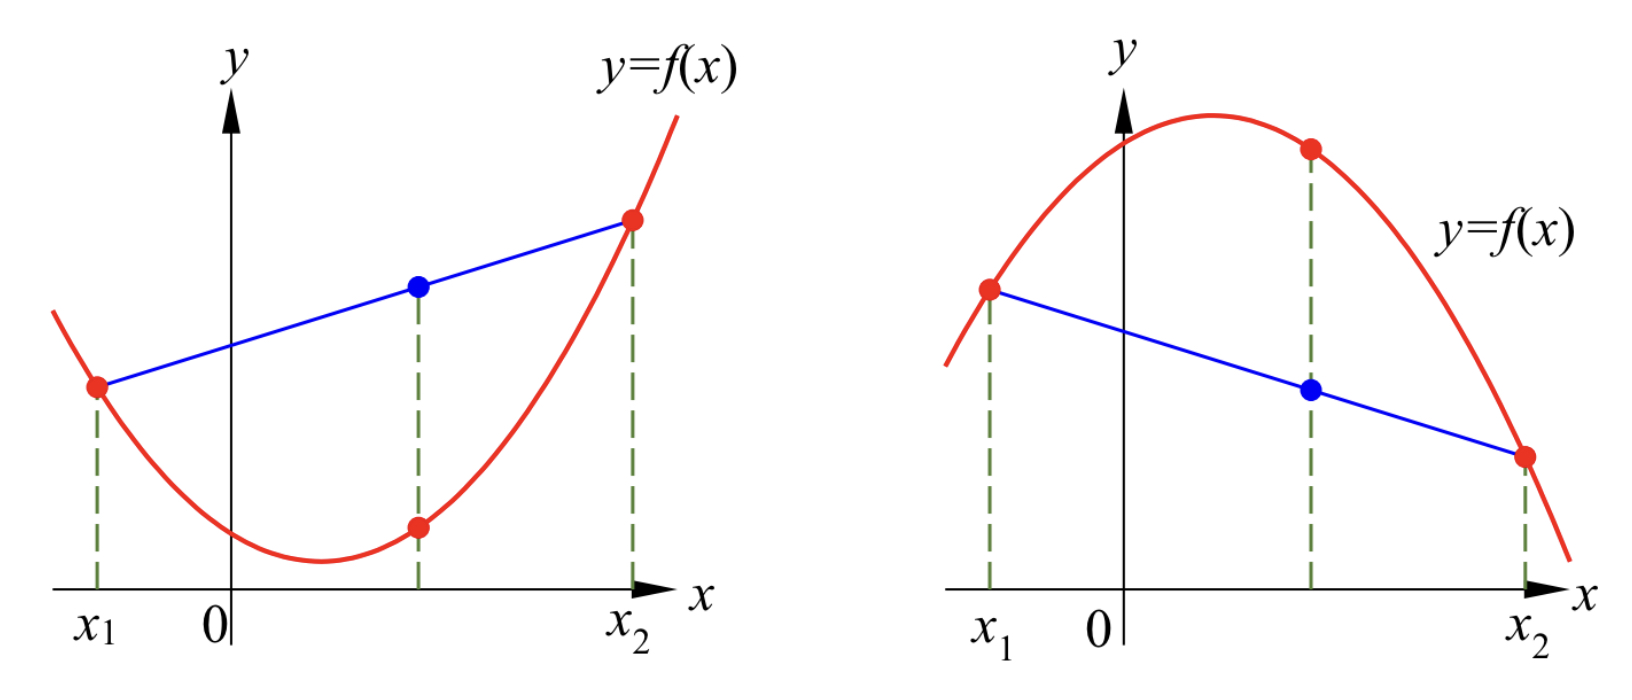
\includegraphics[scale=0.2]{Picture35.png}
\caption{(a) A strictly concave up function. (b)  A strictly concave down function.\fa}\label{figure35}
\end{figure}


\begin{example}{}
For any constants $m$ and $c$, the function $f(x)=mx+c$ is concave up and concave down. It is neither strictly concave up nor strictly concave down.
\end{example}

\begin{example}
{}
Show that the function $f:\mathbb{R}\to\mathbb{R}$, $f(x)=x^2$ is strictly concave up.
\end{example}
\begin{solution}{Solution}
Let $x_1$ and $x_2$ be any two distinct real numbers, and let $t$ be a number in the interval $(0,1)$. Then
\begin{align*}
&f((1-t)x_1+tx_2)-(1-t)f(x_1)-tf(x_2)\\&=(1-t)^2x_1^2+2t(1-t)x_1x_2+t^2x_2^2-(1-t)x_1^2-tx_2^2\\
&=-t(1-t)x_1^2+2t(1-t)x_1x_2-t(1-t)x_2^2\\
&=-t(1-t)(x_1-x_2)^2.
\end{align*}
Since   $(x_1-x_2)^2>0$, $t>0$ and $1-t>0$, we find that
\[f((1-t)x_1+tx_2)-(1-t)f(x_1)-tf(x_2)<0.\]
This proves that $f$ is strictly concave up.
\end{solution}



In the definition of concavity, we do not assume any regularity about the function. If a function is differentiable, we can characterize the concavity of the function in terms of its tangent lines.

For a point $x_0\in (a, b)$, the equation of the tangent line to the curve $y=f(x)$ at $x=x_0$ is
\[y=f(x_0)+f'(x_0)(x-x_0).\] 
We say that the graph of $f$ is   above the tangent line at $x=x_0$ provided that 
\[f(x)\geq f(x_0)+f'(x_0)(x-x_0)\hspace{1cm}\text{for all}\; x\in [a,b].\]
We say that the graph of $f$ is  strictly  above the tangent line at $x=x_0$ except at the tangential point provided that 
\[f(x)> f(x_0)+f'(x_0)(x-x_0)\hspace{1cm}\text{for all}\; x\in [a,b]\setminus \{x_0\}.\] 
Similarly, one can define what it means for the graph of $f$ to be below a tangent line, or strictly below.
\begin{theorem}[label=thm230219_1]{}
 Let  $f:[a, b]\rightarrow\mathbb{R}$  be a   function that is continuous on $[a,b]$, and   differentiable on $(a, b)$. The following three conditions are equivalent.


\begin{enumerate}[(a)]

\item $f'$ is strictly increasing on $(a, b)$.
\item The graph of $f$ is strictly  above every tangent line except at the tangential point.
\item $f$ is strictly concave up.
\end{enumerate}
 
\end{theorem}


\begin{myproof}{Proof}
First we prove (a) $\implies$ (b). Take any $x_0\in (a, b)$. The equation of the tangent line at $x=x_0$ is
\[y=g(x)=f(x_0)+f'(x_0)(x-x_0).\] If $x\in [a, b]$, 
\[f(x)-g(x)=f(x)-f(x_0)+f'(x_0)(x-x_0).\]
When $x\neq x_0$,  mean value theorem implies that there exists $u$ strictly between $x_0$ and $x$ such that
\[f(x)-f(x_0)=f'(u)(x-x_0).\]
Therefore
\[f(x)-g(x)=(x-x_0)(f'(u)-f'(x_0)).\]If $a\leq x<x_0$, $u<x_0$ and so $f'(u)<f'(x_0)$. This implies that $f(x)-g(x)>0$. If $x>x_0$, $u>x_0$ and so $f'(u)>f'(x_0)$. Then we also have $f(x)-g(x)>0$.  In other words, we have proved that for any $x_0$ in $(a, b)$, for any $x\in [a,b]\setminus\{x_0\}$,
\[f(x)>f(x_0)+f'(x_0)(x-x_0).\]\bp
This proves that the graph of $f$ is strictly  above every tangent line except at the tangential point.

Next, we prove (b) $\implies$ (c). Given $x_1$ and $x_2$ in $[a,b]$ with $x_1<x_2$, and $t\in (0,1)$, let $x_0=(1-t)x_1+tx_2$. Then $x_1<x_0<x_2$, and 
\[x_1-x_0=-t(x_2-x_1),\hspace{1cm}x_2-x_0=(1-t)(x_2-x_1).\]
By assumption,
\[f(x_1)>f(x_0)+f'(x_0)(x_1-x_0)=f(x_0)-tf'(x_0)(x_2-x_1),\]
\[f(x_2)>f(x_0)+f'(x_0)(x_2-x_0)=f(x_0)+(1-t)f'(x_0)(x_2-x_1).\]
Therefore,
\[(1-t)f(x_1)+tf(x_2)>f(x_0)=f((1-t)x_1+tx_2).\]
This proves that $f$ is strictly concave up.

Finally, we prove (c) $\implies $ (a). First we will prove that $f'$ is increasing on $(a, b)$. Given $x_1$ and $x_2$ in $(a, b)$ with $x_1<x_2$, we want to show that  $f'(x_1)\leq f'(x_2)$. For any $x\in (x_1, x_2)$, there exists $t\in (0,1)$ such that $x=(1-t)x_1+tx_2$. Since $f$ is strictly concave up, we have
\[f(x)=f((1-t)x_1+tx_2)<(1-t)f(x_1)+tf(x_2).\]
This implies that
\[(1-t)(f(x)-f(x_1))<t(f(x_2)-f(x)).\]
Since $x-x_1=t(x_2-x_1)$ and $x_2-x=(1-t)(x_2-x_1)$, we have
\begin{equation}\label{eq230219_1}\frac{f(x)-f(x_1)}{x-x_1}<\frac{f(x_2)-f(x)}{x_2-x}.\end{equation} Letting $x\to x_1^+$ in \eqref{eq230219_1}, we find that
\[f'(x_1)\leq \frac{f(x_2)-f(x_1)}{x_2-x_1}.\]\bp
Letting $x\to x_2^-$ in \eqref{eq230219_1}, we find that
\[f'(x_2)\geq \frac{f(x_2)-f(x_1)}{x_2-x_1}.\]These prove that
\[f'(x_2)\geq f'(x_1).\]
In other words, we have proved that $f'$ is increasing on $(a,b)$. If $f'$ is not strictly increasing on $(a, b)$, there exist $x_1$ and $x_2$ in $(a, b)$ with $x_1<x_2$ but $f'(x_1)=f'(x_2)$. Since $f'$ is increasing, we will have $f'(x)=f'(x_1)=f'(x_2)=m$ for all $x\in (x_1, x_2)$. This implies that 
\[f(x)=mx+c \hspace{1cm}\text{for all}\; x\in [x_1, x_2].\]
But then for any $t\in (0,1)$,
\[f((1-t)x_1+tx_2)=m\left[(1-t)x_1+tx_2\right]+b=(1-t)f(x_1)+tf(x_2),\]
which constradicts to the strict concavity of $f$. Therefore, $f'$ must be strictly increasing on $(a,b)$.
\end{myproof}

By replacing $f$ by $-f$ in Theorem \ref{thm230219_1}, we obtain the following immediately.
\begin{theorem}[label=thm230219_2]{}
 Let  $f:[a, b]\rightarrow\mathbb{R}$  be a   function that is continuous on $[a,b]$, and   differentiable on $(a, b)$. The following three conditions are equivalent.
\begin{enumerate}[(a)]

\item $f'$ is strictly decreasing on $(a, b)$.
\item The graph of $f$ is strictly below every tangent line except at the tangential point.
\item $f$ is strictly concave down.
\end{enumerate}
 
\end{theorem}

In Theorem \ref{thm230219_1}, if we relax the strictness, the proofs are actually easier.  
\begin{theorem}[label=thm230219_3]{}
 Let  $f:[a, b]\rightarrow\mathbb{R}$  be a   function that is continuous on $[a,b]$, and   differentiable on $(a, b)$. The following three conditions are equivalent.
\begin{enumerate}[(a)]

\item $f'$ is   increasing on $(a, b)$.
\item The graph of $f$ is   above every tangent line.
\item $f$ is  concave up.
\end{enumerate}
 
\end{theorem}

\begin{theorem}[label=thm230219_4]{}
 Let  $f:[a, b]\rightarrow\mathbb{R}$  be a   function that is continuous on $[a,b]$, and   differentiable on $(a, b)$. The following three conditions are equivalent.
\begin{enumerate}[(a)]

\item $f'$ is  decreasing on $(a, b)$.
\item The graph of $f$ is  below every tangent line.
\item $f$ is  concave down.
\end{enumerate}
 
\end{theorem}


If a function is twice differentiable, we can characterize concavity using second derivatives.
\begin{theorem}{}
 Let  $f:[a, b]\rightarrow\mathbb{R}$ be a function that is continuous on $[a,b]$, and twice differentiable on $(a, b)$.
 
\begin{enumerate}[1.]
\item $f(x)$ is   concave up if and only if $f''(x)\geq 0$ for all $x\in (a, b)$.
\item $f(x)$ is   concave down if and only if $f''(x)\leq 0$ for all $x\in (a, b)$.
\item If $f''(x)>0$ for all $x\in (a, b)$,  then $f$ is strictly concave up.

\item  If $f''(x)<0$ for all $x\in (a, b)$, then  $f$ is strictly concave down.

\end{enumerate}
\end{theorem}
\begin{myproof}{Proof}
For (a) and (b),  this is just the fact that $f''(x)\geq 0$ for all $x\in (a, b)$ if and only if $f'$ is increasing;  $f''(x)\leq 0$ for all $x\in (a, b)$ if and only if $f'$ is decreasing.

For (c) and (d), we note that $f''(x)>0$ for all $x\in (a,b)$ implies that $f'$ is strictly increasing on $(a,b)$; while  $f''(x)<0$ for all $x\in (a,b)$ implies that $f'$ is strictly decreasing on $(a,b)$
\end{myproof}
We have seen that if a differentiable function $g:(a,b)\to\mathbb{R}$ is strictly increasing, it is not necessary that $g'(x)>0$ for all $x\in (a,b)$. This is why for $f:(a,b)\to\mathbb{R}$ to be strictly concave up, it is not necessary that $f''(x)>0$ for all $x\in (a,b)$. The function $f:\mathbb{R}\to\mathbb{R}$, $f(x)=x^4$ gives an example of a function that is strictly concave up, but it is not true that $f''(x)>0$ for all $x\in\mathbb{R}$. 
\begin{example}{}
Show that the function $f:[0, \pi]\to\mathbb{R}$, $f(x)=\sin x$ is strictly concave down.
\end{example}
\begin{solution}{Solution}
Since $f''(x)=-\sin x<0$ for all $x\in (0, \pi)$, we find that $f:[0, \pi]\to\mathbb{R}$, $f(x)=\sin x$ is strictly concave down.
\end{solution}
\begin{example}
{}Consider the power function $f(x)=x^r$. Since $f''(x)=r(r-1)x^{r-2}$, we have the following.
\begin{enumerate}[1.]
\item When $r<0$,  the function $f:(0,\infty)\to\mathbb{R}$, $f(x)=x^r$ is strictly concave up. 
\item When $0<r<1$, the function $f:[0,\infty)\to\mathbb{R}$, $f(x)=x^r$ is strictly concave down. 
\item When $r>1$, the  function $f:[0,\infty)\to\mathbb{R}$, $f(x)=x^r$ is strictly concave up.\end{enumerate}
\end{example}

Next we look at a classical example where the concavity of a function can be used to prove inequalities.
\begin{example}{Young's Inequality}
Given that $p$ and $q$ are positive numbers such that
\[\frac{1}{p}+\frac{1}{q}=1.\]If $a$ and $b$ are positive numbers, show that 
\[ab\leq \frac{a^p}{p}+\frac{b^q}{q}.\]Equality holds if and only if $a^p=b^q$.
\end{example}
\begin{solution}{Solution}Notice that since $p$ and $q$ are positive, we have $1/p<1$ and $1/q<1$. This implies that $p>1$ and $q>1$.
Consider the function $f:(0,\infty)\to\mathbb{R}$, $f(x)=\ln x$. We find that
\[f'(x)=\frac{1}{x},\quad f''(x)=-\frac{1}{x^2}<0\hspace{1cm}\text{for all}\; x>0.\]  Hence, the function $f:(0,\infty)\to\mathbb{R}$, $f(x)=\ln x$ is strictly concave down. 
This implies that for any two   positive numbers $x_1$ and $x_2$, and any $t\in (0,1)$, 
\begin{equation}\label{eq230219_5}\ln \left((1-t)x_1+tx_2\right)\geq (1-t)\ln x_1+t\ln x_2.\end{equation} The equality can hold if and only if $x_1=x_2$.   Now, let
$t=1/q$.
Then $t\in (0,1)$ and $1-t=1/p$. Given the positive numbers $a$ and $b$, let
\[x_1=a^p, \quad x_2=b^q.\]
 Then $x_1$ and $x_2$ are positive numbers. Eq. \eqref{eq230219_5} implies that
\[\ln \left(\frac{a^p}{p}+\frac{b^q}{q}\right)\geq \frac{1}{p}\ln a^p+\frac{1}{q}\ln b^q=\ln (ab),\]\bs with equality holds if and only if $a^p=b^q$. Therefore,
\[ab\leq \frac{a^p}{p}+\frac{b^q}{q}.\]Equality holds if and only if $a^p=b^q$.
\end{solution}

\vp
\noindent
{\bf \large Exercises  \thesection}
\setcounter{myquestion}{1}
\begin{question}{\themyquestion}
\begin{enumerate}[(a)]
\item Show that the function $f:\mathbb{R}\to \mathbb{R}$, $f(x)=e^{-x}$ is strictly concave up.
\item Show that the function $f:(0,\pi)\to \mathbb{R}$, $f(x)=\di\frac{1}{\sin x}$ is strictly concave up.
\end{enumerate}
\end{question}


 \atc
\begin{question}{\themyquestion}
Let $f:(a,b)\to\mathbb{R}$ be a twice differentiable function. If $f:(a,b)\to\mathbb{R}$ is concave down, and $f(x)>0$ for all $x\in (a, b)$, prove that the function $g:(a,b)\to\mathbb{R}$,
\[g(x)=\frac{1}{f(x)}\] is concave up.
\end{question}

\atc
\begin{question}{\themyquestion}
Given that the function $f:[a,b]\to\mathbb{R}$ is concave down. Show that for any  $x_1, x_2, \ldots, x_n$ in $[a, b]$, if  $t_1, t_2, \ldots, t_n$ are nonnegative numbers satifying \[t_1+t_2+\ldots+t_n=1,\]then
\[f(t_1x_1+t_2x_2+\cdots+t_nx_n)\geq t_1f(x_1)+t_2f(x_2)+\cdots+t_nf(x_n).\]
 
\end{question}

\atc
\begin{question}{\themyquestion: Arithmetic Mean-Geometric Mean Inequality}
The arithmetic mean-geometric mean inequality states that if $a_1, a_2, \ldots, a_n$ are $n$ positive numbers, then
\[\frac{a_1+a_2+\cdots+a_n}{n}\geq \sqrt[n]{a_1a_2\cdots a_n}.\]
Use the concavity of the function $f:(0,\infty)\to\mathbb{R}$, $f(x)=\ln x$ and the result of the previous question to prove this inequality.
 
\end{question}